%\documentclass{article}
\documentclass{report}
%\usepackage[utf8]{vietnam}
\usepackage[utf8]{inputenc}
\usepackage[T5]{fontenc}
\usepackage{anyfontsize,fontsize}
\changefontsize[13pt]{13pt}	
\usepackage{commath}
\usepackage{parskip,setspace}
\usepackage{xcolor}
\usepackage{amssymb}
\usepackage[d]{esvect}
\usepackage[nottoc,notlot,notlof]{tocbibind}
\usepackage{slashed,cancel}
\usepackage{indentfirst,titlesec}
\usepackage{pdfpages}
\usepackage{graphicx,subcaption,floatrow,adjustbox,rotating}
\usepackage{nccmath}
\usepackage{mathtools}
\usepackage{amsfonts,esint}
\usepackage[printonlyused,withpage]{acronym}
\usepackage{wrapfig}
\usepackage[toc,page]{appendix}
\usepackage{amsmath,systeme}
\usepackage[thinc]{esdiff}
\usepackage{hyperref,tikz}
\usepackage{bm,physics,nicematrix}
\usepackage[numbers,comma,sort&compress]{natbib}
%footnote
\usepackage{fancyhdr}
\usepackage{array,tocbibind}
\usepackage{enumitem}
\pagestyle{empty}


\usepackage{geometry}
\geometry{
a4paper,
total={170mm,257mm},
left=20mm,
top=20mm,
}



\newcommand{\image}[1]{
\begin{center}
	\includegraphics[width=0.5\textwidth]{pic/#1}
\end{center}
}




\renewcommand{\l}{\ell}
\newcommand{\dps}{\displaystyle}

\newcommand{\f}[2]{\dfrac{#1}{#2}}
\newcommand{\at}[2]{\bigg\rvert_{#1}^{#2} }


\renewcommand{\baselinestretch}{1.5}



\hypersetup{
colorlinks=true,
linkcolor=black,
filecolor=magenta,      
urlcolor=cyan,
pdftitle={UT},
citecolor=green,
pdfpagemode=FullScreen,
}

\urlstyle{same}

\titleformat{\chapter}[display]
{\centering\large\bfseries} 
{\textbf{\MakeUppercase{\chaptername}} \ \thechapter\vspace{15pt}}{20pt}
{\large} 

%\newcommand{\thesistitlee}{Three-band tight binding model for TMD monolayers in the presence of a magnetic field}
\newcommand{\thesistitlee}{Hofstadter butterfly in transistion metal dichalcogenide monolayers}
\newcommand{\address}{NATIONAL UNIVERSITY OF HO CHI MINH CITY UNIVERSITY OF SCIENCE}
\newcommand{\department}{FACULTY OF PHYSICS - ENGINEERING PHYSICS}
\newcommand{\thesisauthor}{Tran Khoi Nguyen}
\newcommand{\thesisadvisor}{Your Advisor's Name}
\newcommand{\graddate}{Ho Chi Minh City, 2025}
\newcommand{\thesisdedication}{To all the Ph.D. pursuing brave souls}

\newlist{abbrv}{itemize}{1}
\setlist[abbrv,1]{label=,labelwidth=1in,align=parleft,itemsep=0.1\baselineskip,leftmargin=!}
\begin{document}
\setlength{\parindent}{20pt}
\begin{titlepage}
	\begin{center}
		{\bfseries

		{\large {\bf \address}}\\
		{{\textbf{\department}}}\\
		{---------------------o0o--------------------}
		\vspace{1.5cm}

		{\large {\bf UNDERGRADUATE THESIS}}\\
		\vspace{3.0cm}

		}

	\end{center}
	\textit{\textbf{\underline{Thesis title:}}}\\
	\begin{center}
		{\bfseries

			{\largerrr\thesistitlee}
			\vspace{1in}

		}
	\end{center}
	\noindent
	\makebox[\textwidth]{\hfill\makebox[3in]{\hrulefill}}\\
	\begin{center}
		\makebox[\textwidth]{\hfill\makebox[3in]{\hfill \textbf{Student: Tran Khoi Nguyen}\hfill}}
		\makebox[\textwidth]{\hfill\makebox[3in]{\hfill \textbf{Supervisor: Dr. Huynh Thanh Duc}\hfill}}
	\end{center}
	\begin{tikzpicture}[remember picture, overlay]
		\draw[line width=2pt]
		([xshift=1.5cm, yshift=1.5cm] current page.south west)
		rectangle
		([xshift=-1.5cm, yshift=-1.5cm] current page.north east);
	\end{tikzpicture}
	\begin{center}
		\vspace{2.5in}
		{\graddate}
	\end{center}
\end{titlepage}
\begin{titlepage}
	\begin{center}
		{\bfseries

		{\large {\bf \address}}\\
		{{\textbf{\department}}}\\
		\vspace{2.5cm}

		{\large {\bf UNDERGRADUATE THESIS}}\\
		\vspace{3.0cm}

		}

	\end{center}
	\textit{\textbf{\underline{Thesis title:}}}\\
	\begin{center}
		{\bfseries

			{\largerrr\thesistitlee}
			\vspace{0.5in}

		}
	\end{center}
	\parbox{3cm}{Major code:\\ Specialization:}\parbox{5cm}{7440102\\Theoretical Physics}\\[1cm]
	\noindent
	\makebox[\textwidth]{\hfill\makebox[3in]{\hrulefill}}\\
	\begin{center}
		\makebox[\textwidth]{\hfill\makebox[3in]{\hfill \textbf{Student: Tran Khoi Nguyen}\hfill}}
		\makebox[\textwidth]{\hfill\makebox[3in]{\hfill \textbf{Supervisor: Dr. Huynh Thanh Duc}\hfill}}
	\end{center}
	\begin{center}
		\vspace{2.5in}
		{\graddate}
	\end{center}
\end{titlepage}

\newpage
\pagenumbering{roman}
\pagestyle{fancy}
\renewcommand{\headrulewidth}{0pt}
\fancyhf{}
\fancyfoot[C]{\hspace{0cm} \thepage}
\setcounter{page}{1}

\chapter*{GUARANTEE}
I guarantee to indepentdently conducting the calculation of the Hofstadter butterfly of an ideal two-dimensional system of MoS$_{2}$ for my bachelor thesis, under the supervision of Dr. Huynh Thanh Duc.

The contexts are included in this graduation thesis are totally accurate and honest. \\[2cm]



\parbox{0.75in}{\centering \textbf{}} \hfill \parbox{4in}{\centering \textbf{STUDENT}\\
\textit{(Signature)}\\[2cm] Tran Khoi Nguyen}

\chapter*{ACKNOWLEDGMENTS}
This thesis would not have been possible without the help and support of a large number of individuals. Firstly, I would like to thank my family members, especially my beloved mother and my sister, who have totally encouraged me on my path of becoming a scientist and helped me trenmendously in all ways possible. Without them, I would not have enough much confidence to finish this. Thank you.

I am deeply greeted to my supervisor Dr. Huynh Thanh Duc from the Institute of Physics, Ho Chi Minh city, who taught me not only knowledges, gave me advise but also wholeheartedly encouraged and guided me every steps of the way. I would like to thank Master Le Minh Chau from the Institute of Physics and Vo Chau Duc Phuong from ICTP, who helped me at the very first step of this thesis. I would also like to acknowledge with gratitude to Dr. Vu Quang Tuyen, Dr. Vo Quoc Phong and Dr. Nguyen Huu Nha from the Department of Theoretical Physics. They have trully inspired me on the way becoming a physicist.

Finally, I would like to thank my colleagues at the University of Science including Dao Duy Tung, Le Quoc Duy, Ho Ngo Thanh Khoa, Pham Hoang Minh Quang, Truong Anh Duy, Pham Nguyen Thanh Dat. \\ [2cm]


\parbox{0.75in}{\centering \textbf{}} \hfill \parbox{4in}{\centering \textit{Ho Chi Minh city, July, 2025}\\ \textbf{Tran Khoi Nguyen}}


\renewcommand{\contentsname}{TABLE OF CONTENTS}
\tableofcontents
\renewcommand{\listfigurename}{LIST OF FIGURES}
\listoffigures
\newpage
\renewcommand{\listtablename}{LIST OF TABLES}
\listoftables
\newpage
\chapter*{\MakeUppercase{List of Abbreviations}}
%\addcontentsline{toc}{chapter}{LIST OF ABBREVIATIONS}
\chaptermark{List of Abbreviations}
\begin{acronym} % Give the longest label here so that the list is nicely aligned
	\acro{LCAO}{Linear Combination of Atomic Orbital}
	\acro{TMD}{transition metal dichacolgenides}
	\acro{TB}{tight-binding}
	\acro{TBM}{tight-binding model}
	\acro{NN}{nearest-neighbor}
	\acro{NNN}{next nearest-neighbor}
	\acro{TNN}{third-nearest-neighbor}
	\acro{2D}{two-dimensional}
	\acro{BZ}{Brillouin zone}
	\acro{GGA}{generalized-gradient approximation}
	\acro{LDA}{local-density approximation}
	\acro{SOC}{spin orbit coupling}
	\acro{LL}{Landau levels}
	\acro{QHE}{Quantum Hall effect}
	\acro{IQHE}{integer Quantum Hall effect}
	\acro{FQHE}{fractional Quantum Hall effect}
	\acro{EFA}{Envelope Function Approximation}
	\acro{BCH}{Baker-Campbell-Hausdorff}
	\acro{TKNN}{Thouless-Kohmoto-Nightingale-Nijs}
	\acro{DOS}{Density of state}
  	\acro{VB}{valence band}
  	\acro{CB}{conduction band}
	\end{acronym}
\newpage
\chapter*{Abstract}
%\textbf{ABSTRACT}

Hofstadter's butterfly has been studied experimentally for 50 years. It was first discovered by computer scientist Douglas Hofstadter. This thesis explores the electronic phenomena in material systems, particularly focusing on monolayer transistion metal dichacolgenides. We begin by studying a minimal three-band \ac{TBM} in order to describe the electronic structure of TMD monolayer. In the presence of an external magnetic field, the calculated band energies show Landau levels at small fields and become fractal-structured at strong fields, which is known as the Hofstadter butterfly. Building on this framework, we further explore related quantum phenomena including Landau levels and quantum Hall effect.\\
\textbf{Keywords}: Tight-binding model, Hofstadter butterfly, Honeycomb lattice, Landau levels, quantum Hall effect, transistion metal dichacolgenides.

{\fontencoding{T5}\selectfont 
\chapter*{Tóm tắt}
Phổ năng lượng Hofstadter đã được nghiên cứu thực nghiệm trong suốt 50 năm qua. Hiện tượng này lần đầu tiên được phát hiện bởi nhà khoa học máy tính Douglas Hofstadter. Khóa luận này tập trung nghiên cứu các hiện tượng điện tử trong các hệ vật liệu, đặc biệt là lớp đơn của các hợp chất chuyển tiếp kim loại – dichalcogenide. Trước tiên, chúng tôi khảo sát một mô hình ba dải tối giản theo phương pháp liên kết chặt nhằm mô tả cấu trúc điện tử của đơn lớp TMDC. Khi đặt vào một từ trường ngoài, các mức năng lượng được tính toán thể hiện sự hình thành của các mức Landau ở cường độ từ trường yếu và xuất hiện cấu trúc fractal đặc trưng khi từ trường mạnh – hiện tượng được gọi là \textit{Hofstadter butterfly}. Dựa trên mô hình này, chúng tôi tiếp tục khảo sát các hiện tượng lượng tử có liên quan như các mức Landau và hiệu ứng Hall lượng tử.
}


\newpage
\pagenumbering{arabic}
\chapter{\textbf{INTRODUCTION}}
Since the isolation of graphene in 2004, research on the field of \ac{2D} materials has noticeably grown into a major branch of physical science with a wide range of applications. Their unique \ac{2D} structure offers an open canvas to tailor and functionalize through layer number, defects, morphology, moir\'e patterns, strain, and other tunable properties. \ac{2D} materials, such as graphene and monolayer \ac{TMD}, have become a focal point in condensed matter physics due to their extraordinary electronic properties. Over the years, researchers have focused on graphene, with hope that its potential to replace silicon, enabling the continuation of Moore's law in next-generation semiconductor devices. However, in recent years, owing to their potentials, the number of scholarly papers researching graphene's use was enormous, reached a peak of thousand publications annually in 2021. Meanwhile, \ac{TMD} have created tremendous interest among materials scientists, on account of their huge potential for new types of electronics, optoelectronics and superconductivity. Atomically thin \ac{2D} \ac{TMD} have led to a variety of promising technologies for nanoelectronic, sensing and optoelectronics. Unlike graphene, many \ac{2D} \ac{TMD} are naturally semiconductors and enormously posses potential to be made into ultra-small and low power transistors than silicon. These materials consist of large atom from the transistion metal elements that lies in the middle of the periodic table are sandwiched by two layers of atoms from the chalcogenide elements, such as sulfur or selenium, forming a three-layer sandwich called a transistion metal dichalcogenides.

Another majority opportunity is unraveling the fundamental behind the unique properties of \ac{2D} materials. These systems exhibit a various interesting quantum effects, such as superconductivity, weak localization, tological insulation, and others. In some cases, these quantum effects can lead to novel applications, such as valleytronics or twistronics.

The Hofstadter butterfly have been studied for nearly 50 years with various ranging reportly from \ac{2D} symmetry lattice such as square lattice, triangular lattice, honeycomb lattice, Kagome lattice to Lieb's lattice, Mielke's lattice, Tasaki's lattice under an uniform magnetic field. The first Hofstadter butterfly was originally made for an electron moving in a \ac{2D} square lattice by computer scientist Douglas Hofstadter. The behaviour of an electron in such a quantum system could produce an energy spectrum which leads to a self-similar recursive Landau level spectrum resembling butterfly swings. The idea behind Hofstadter’s butterfly is that you’re looking at how the band structure of electrons moves when you have the magnetic field on one axis and the electrons’ energies on the other, and plotted on that diagram, the band forms a fractal structure that looks like a butterfly.

This thesis is mainly organized to explore the electronic structure of \ac{2D} material systems under external magnetic fields, with a particular focus on monolayer \ac{TMD}. 

We begin in Chapter~2 by presenting the theoretical background, including the tight-binding model, the crystal structure of \acp{TMD}, Landau quantization, and the Hall effect.

In Chapter~3, we study the three-band tight-binding model introduced in Ref.~\cite{PhysRevB.88.085433}, and then extend it by incorporating the effects of an external magnetic field.

Chapter~4 presents the results obtained from the model developed in Chapter~3. A portion of these results has been previously reported by other research groups Refs.~\cite{ho2014,ho2015}, but we also include new findings and a more general approach that broadens the scope of the original model. A key novelty of this work lies in the integration of theoretical elements from Chapter~2, such as Hall effects. To the best of our knowledge, such an explicit incorporation has not been addressed in the existing literature. This theoretical refinement enables a more systematic and physically grounded analysis of the Hofstadter spectrum in monolayer \acp{TMD}.



% Based on the minimal model introduced in Ref. \cite{PhysRevB.88.085433} we derived the tight-binding Hamiltonian without magnetic field and computed the bandstructure for \ac{TMD} monolayers. In Section 2.2, we first meets the Hofstadter butterfly of monolayer \ac{TMD} by deriving the Hamiltonian in the tight-binding model under a fractional magnetic field and analyzing the result Hofstadter spectrum. Delving into the Hofstadter physics, we begin exploring the butterfly with quantum phenomena such as Landau levels and quantum Hall effects. These are disscused in Section. 2.2 and Section 2.3. The results obtained exhibits an interesting phenomana. Ultimately, chapter 3 concludes the thesis by summarizing the focus key finding and highlighting the potential avenues for future research. This includes the exploration of interaction effects beyond tight-binding theory and the extension of material physics studies to other tunable properties, such as Moir\'e systems or twisted bilayer systems to \ac{2D} materials.

\chapter{\textbf{THEORY FRAMEWORK}}
In this chapter, we present the theoretical background underpinning the study, commencing with an introduction to the tight-binding method as the main approach to describe the electronic structure of \acp{TMD}. The crystal structure of \acp{TMD} is also discussed to determine their symmetries. Additionally, in the presence of a magnetic field, electronic motion becomes quantized into Landau levels, as first proposed by Lev Landau. Following this, we also present the theoretical framework of the Hall effect, beginning with the classical Hall effect and culminating with the quantum Hall effect, as presented in Ref.~\cite{klitzing90}. The study of Hall effect based largely on the treatment in Ref.~\cite{xiao2010berry}.


\section{The tight-binding method}\label{Section 2.1}
The tight-binding approximation is based on the \ac{LCAO} method. This approach constructs electronic wave functions using the atomic orbitals of isolated atoms. In the tight-binding method, we assume the electrons stay close to the atomic sites and the overlap between neighboring orbitals is small.\\
We start with the single electron time-indepentdent Schr\"{o}dinger equation
\begin{gather}
	H_{\text{1e}} \psi = \left[-\f{\hbar^{2} \nabla^{2}}{2m} + U_{0}(\mathbf{r})\right] \psi_{\lambda,\mathbf{k}}(\mathbf{r}) = \varepsilon_{\lambda}(\mathbf{k}) \psi_{\lambda,\mathbf{k}}(\mathbf{r}),
\end{gather}
where $U_{0}(\mathbf{r})$ is the periodic lattice potential, $\psi_{\lambda,\mathbf{k}}(\mathbf{r})$ is the Bloch wavefunction of an electron in band $\lambda$ with wave vector $\mathbf{k}$ and $\varepsilon_{\lambda}(\mathbf{k})$ is the energy dispersion in crystal. In the \ac{LCAO} method, the electronic wave function can be written as 
\begin{gather}
	\psi_{\text{LCAO}} = \frac{1}{\sqrt{N}}\sum_{n = 1}^{N} \sum_{i = 1}^{N_{i}} \sum_{j = 1}^{N_{\text{orb}}} c_{j,i}(\mathbf{R}_{n}) \phi_{j} (\mathbf{r} - \mathbf{R}_{n} - \mathbf{r}_{i}),
\end{gather}
in which $\phi_{j}$ is the orbital wave function $j$ of an atomic $i$ localized on a lattice site $\mathbf{R}_{n}$. Here, $ N_{\text{orb}} $ is the number of orbitals per atom, $ N_{i} $ is the number of atoms in the unit cell, and $ N $ is the number of unit cells.

As for the \acf{TBM} and the \ac{LCAO} theory, the single electron Bloch wave function can be expressed in terms of atomic orbitals as follows
\begin{gather}
	\psi_{\lambda,\mathbf{k}}(\mathbf{r}) = \frac{1}{\sqrt{N}} \sum_{n=1}^{N} \sum_{i = 1}^{N_{i}} \sum_{j = 1}^{N_{\text{orb}}} C_{j,i}^{\lambda} (\mathbf{k})  e^{i \mathbf{k} (\mathbf{R_{n}} + \mathbf{r}_{i})} \phi_{j} (\mathbf{r} - \mathbf{R}_{n} - \mathbf{r}_{i}) ,
\end{gather}
here, $C_{ji}^{\lambda}(\mathbf{k})$ are the coefficients of linear expansion.

Thanks to the wave function found in Eq.~(2.2), now we apply $e^{-i \mathbf{k} \cdot \mathbf{r}_{i'}} \phi_{j'}^{*}(\mathbf{r} - \mathbf{r}_{i'})$ to the left of the single electron Schr\"{o}dinger Eq.~(2.1) and taking the sum over $\mathbf{r}$
\begin{gather}
	\sum_{i = 1}^{N_{i}} \sum_{j = 1}^{N_{\text{orb}}} \left( H_{j' i', j i}(\mathbf{k}) - \varepsilon(\mathbf{k}) S_{j' i', j i}(\mathbf{k}) \right) C_{j,i}^{\lambda}(\mathbf{k}) = 0,
\end{gather}
where
\begin{gather}
	H_{ji,ji}(\mathbf{k}) =  \int \phi_{j}^{*}(\mathbf{r} - \mathbf{r}_{i}) H_{1\text{e}} \phi_{j}({\mathbf{r} - \mathbf{r}_{i}}),
\end{gather}
is the on-site energy,
\begin{gather}
	H_{j'i',ji}(\mathbf{k}) =  \sum_{n = 1}^{N} e^{i \mathbf{k} \cdot (\mathbf{R}_{n} + \mathbf{r}_{i} - \mathbf{r}_{i'})} \int \phi_{j'}^{*}(\mathbf{r} - \mathbf{r}_{i'}) H_{1\text{e}} \phi_{j}({\mathbf{r} - \mathbf{R}_{n} - \mathbf{r}_{i}}),
\end{gather}
is the hopping energy,
\begin{gather}
	S_{j'i',ji}(\mathbf{k}) =  \sum_{n = 1}^{N} e^{i \mathbf{k} \cdot (\mathbf{R}_{n} + \mathbf{r}_{i} - \mathbf{r}_{i'})} \int \phi_{j'}^{*}(\mathbf{r} - \mathbf{r}_{i'})  \phi_{j}({\mathbf{r} - \mathbf{R}_{n} - \mathbf{r}_{i}}),
\end{gather}
is the overlap integral. 
The terms $H_{j'i',ji}$ and $H_{ji,ji}$ are called the Hamiltonian matrix elements. The solution of the Eq.~(2.4) is the eigenvalue $\varepsilon$ of the Schr\"{o}dinger Eq.~(2.1). Each eigenvalue give an energy dispersion of the system, called the energy band. 

The term in Eq.~(2.6) is often referred to as the \emph{hopping parameter}, which characterizes the strength of the interaction between atoms at positions $ i $ and $ i' $. A larger value implies stronger bonding and easier electron transfer between the atoms. In tight-binding theory, these matrix elements are often obtained from experimental data and treated as semi-empirical parameters.
\section{Crystal structure of TMDs}

\begin{figure}[H]
	\centering
	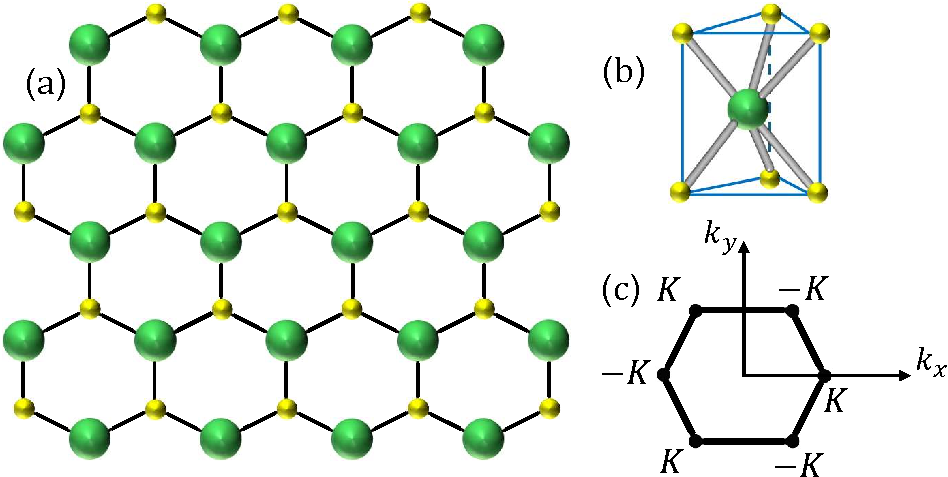
\includegraphics[width=\linewidth]{pic/latticePresent.pdf}
	\caption[Structure of TMD.]{\label{fig:Lattice}Structure of TMD. (a) Top view of monolayer MX$_{2}$. (b) sideview of monolayer MX$_{2}$. The green spheres represent M atoms, which are sandwiched by two layer of X atoms (yellow spheres). (c) The first Brillouin zone and high symmetry points in $k$-space.}
\end{figure}
Monolayer \acp{TMD} are \ac{2D} materials composed of transition metal and chalcogen atoms arranged in a honeycomb lattice, as illustrated in Fig.~2.1. These materials exhibit $D_{3h}$ point group symmetry \cite{mattheiss1973}. It were first studied in their buld forms as early as the 1960s, mainly in the context of solid-state and materials science. However, scientists moved their interested in monolayer TMDs, i.e, their \ac{2D} form, began to grow significantly after the isolation of graphene in 2004.

In monolayer \acp{TMD}, each transition metal (M) atom contributes five $d$-orbitals: $d_{z^{2}}$, $d_{x^{2} - y^{2}}$, $d_{xy}$, $d_{xz}$, and $d_{yz}$, while each chalcogen (X) atom contributes three $p$-orbitals: $p_{x}$, $p_{y}$, and $p_{z}$. The transition metal atoms form a triangular lattice and are sandwiched between two layers of chalcogen atoms, which themselves are arranged on a triangular lattice at alternating hollow sites. This arrangement results in a trigonal prismatic coordination, where each metal atom is surrounded by six chalcogen atoms positioned at the vertices of a trigonal prism, as shown in Fig.~2.1(b). The top view of monolayer \acp{TMD} is shown in Fig.~2.1(a). The Bravais lattice is spanned by the basis vectors
\begin{gather}
	\vv{a}_{1} = (a,0,0), \vv{a}_{2} = \left( \frac{a}{2}, \frac{\sqrt{3}}{2}a,0 \right),
\end{gather}
where $a$ is lattice constant. The first Brillouin zone of the \ac{TMD} is hexagonal with the high-symmetry points are defined as follows: $\Gamma = (0,0), K = (\tfrac{4\pi}{3a},0)$ and $M = (\tfrac{\pi}{a}, \tfrac{\pi}{\sqrt{3}a})$.





\section{Landau level in magnetic field}
The concept of Landau levels was first introduced by Lev Landau in 1930, describing the quantization of electronic motion in a two-dimensional electron gas under a perpendicular magnetic field. In this section, we briefly revisit the derivation of the Landau level spectrum from the single-particle Hamiltonian, providing a general theoretical overview that lays the foundation for the more complex tight-binding calculations presented later in this thesis.

We begin with the single particle Hamiltonian
\begin{gather}
	H = \frac{\mathbf{p}^{2}}{2m},
\end{gather}
where we apply the substitution
\begin{gather}
	\mathbf{p} \to \mathbf{p} = \boldsymbol{\Pi} + e \mathbf{A}(\mathbf{r}),
\end{gather}
with $\mathbf{A}(\mathbf{r})$ specified in the Landau gauge as $\mathbf{A} = (0, Bx, 0)$. The Hamiltonian then becomes
\begin{equation}
	\begin{aligned}
		H &= \frac{1}{2m} \left(\boldsymbol{\Pi} + e\mathbf{A}(\mathbf{r})\right)^2 \\
		&= \frac{\Pi_{x}^{2}}{2m} + \frac{(\Pi_{y} + eBx)^2}{2m}.
	\end{aligned}
\end{equation}

To diagonalize this Hamiltonian, we define the following ladder operators
\begin{equation}
	\begin{aligned}
		a &= \sqrt{\frac{1}{2\hbar eB}} \left(\Pi_{x} + i \Pi_{y}\right), \\
		a^{\dagger} &= \sqrt{\frac{1}{2\hbar eB}} \left(\Pi_{x} - i \Pi_{y}\right), \\
		b &= \sqrt{\frac{eB}{2\hbar}} \left(y - \frac{1}{eB} \Pi_{x} + i x\right), \\
		b^{\dagger} &= \sqrt{\frac{eB}{2\hbar}} \left(y - \frac{1}{eB} \Pi_{x} - i x\right).
	\end{aligned}
\end{equation}
The inverse transformations read
\begin{equation}
	\begin{aligned}
		\Pi_{x} &= \sqrt{\frac{\hbar eB}{2}} (a + a^{\dagger}), \\
		\Pi_{y} &= i\sqrt{\frac{\hbar eB}{2}} (a^{\dagger} - a).
	\end{aligned}
\end{equation}
The operators $a$ and $a^{\dagger}$ satisfy the bosonic commutation relation
\begin{gather}
	[a, a^{\dagger}] = 1, \quad [a, a] = [a^{\dagger}, a^{\dagger}] = 0.
\end{gather}
Operators $b$ and $b^{\dagger}$ also obey:
\begin{gather}
	[b, b^{\dagger}] = 1, \quad [b, b] = [b^{\dagger}, b^{\dagger}] = 0,
\end{gather}
and in addition, the $a$ and $b$ sectors commute:
\begin{gather}
	[a, b] = [a, b^{\dagger}] = [a^{\dagger}, b] = [a^{\dagger}, b^{\dagger}] = 0.
\end{gather}

As in the one-dimensional harmonic oscillator, the ladder operators act as
\begin{equation}
	\begin{aligned}
		a \ket{n} = \sqrt{n} \ket{n-1}, \quad a^{\dagger} \ket{n} = \sqrt{n+1} \ket{n+1},
	\end{aligned}
\end{equation}
where $\ket{n}$ is an eigenstate of the number operator $a^{\dagger}a$ with eigenvalue $n \geq 0$.

The Hamiltonian in Eq.~(2.11) can now be written in terms of $a$ and $a^{\dagger}$ as
\begin{gather}
	H = \hbar \omega_c \left(a^{\dagger} a + \frac{1}{2}\right), \quad \text{with } \omega_c = \frac{eB}{m}.
\end{gather}
The eigenvalues of Eq.~(2.18) are known as \acp{LL}
\begin{gather}
	E_{n} = \left(n + 1/2\right) \hbar \omega_{c},
\end{gather}
where $n$ is the Landau level index and $\omega_{c}$ is called the cyclotron frequency. These quantized energy are known as \acp{LL}. Each level labeled by the index $n$. The Fig.~2.2 illustrates the Landau level energy spectrum as a function of magnetic field strength. Each line represents a discrete energy level labeled by the Landau index $n$. As the magnetic field $B$ increases, the spacing between adjacent grows linearly due to the dependence of the cyclotron frequency $\omega_{c}$. At zero field, the spectrum is continous, corresponding to the free electron case. However, in the presence of magnetic field, the energy is quantized into discrete levels, leading to the characteristic ladder-like structure shown in the figure.

\begin{figure}[H]
	\centering
	\includegraphics[width=0.5\linewidth]{pic/LLDEMO.pdf}
	\caption[Landau levels.]{Representation of the Landau levels of Eq.~2.19.}
\end{figure}

%These levels give rise to what is called ``the Landau fan'', being very important in the de Haas-van Alphen and Shubnikov-de Haas effects \cite{10.1119/1.1615568} which predicts oscillations of the magnetic moment of a meltal depending on an applied magnetic field.


%More interesting is the top and bottom of conduction and valence band of the zero field spectrum. This results in a non-standard Landau levels when the field is turned on, as discused above.\\
%In the one-band case, knowing the effective mass in zero field and the charge is enough to determine the Landau level spectruc to linear order in the magnetic field. For the three-band case
%
%
% In order to determine the cyclotron frequency for the three-band, through the derivation in Appendix C, we have obtained the Landau levels for the three-band model when the field is turned on
%\begin{figure*}[htb]
%	\centering
%	\begin{subfigure}[b]{0.49\textwidth}
%		\centering
%		{\includegraphics[width=0.85\textwidth,height=1.2\linewidth]{pic/small_area_LL_3band.png}}
%	\end{subfigure}
%	\begin{subfigure}[b]{0.49\textwidth}
%		\centering
%		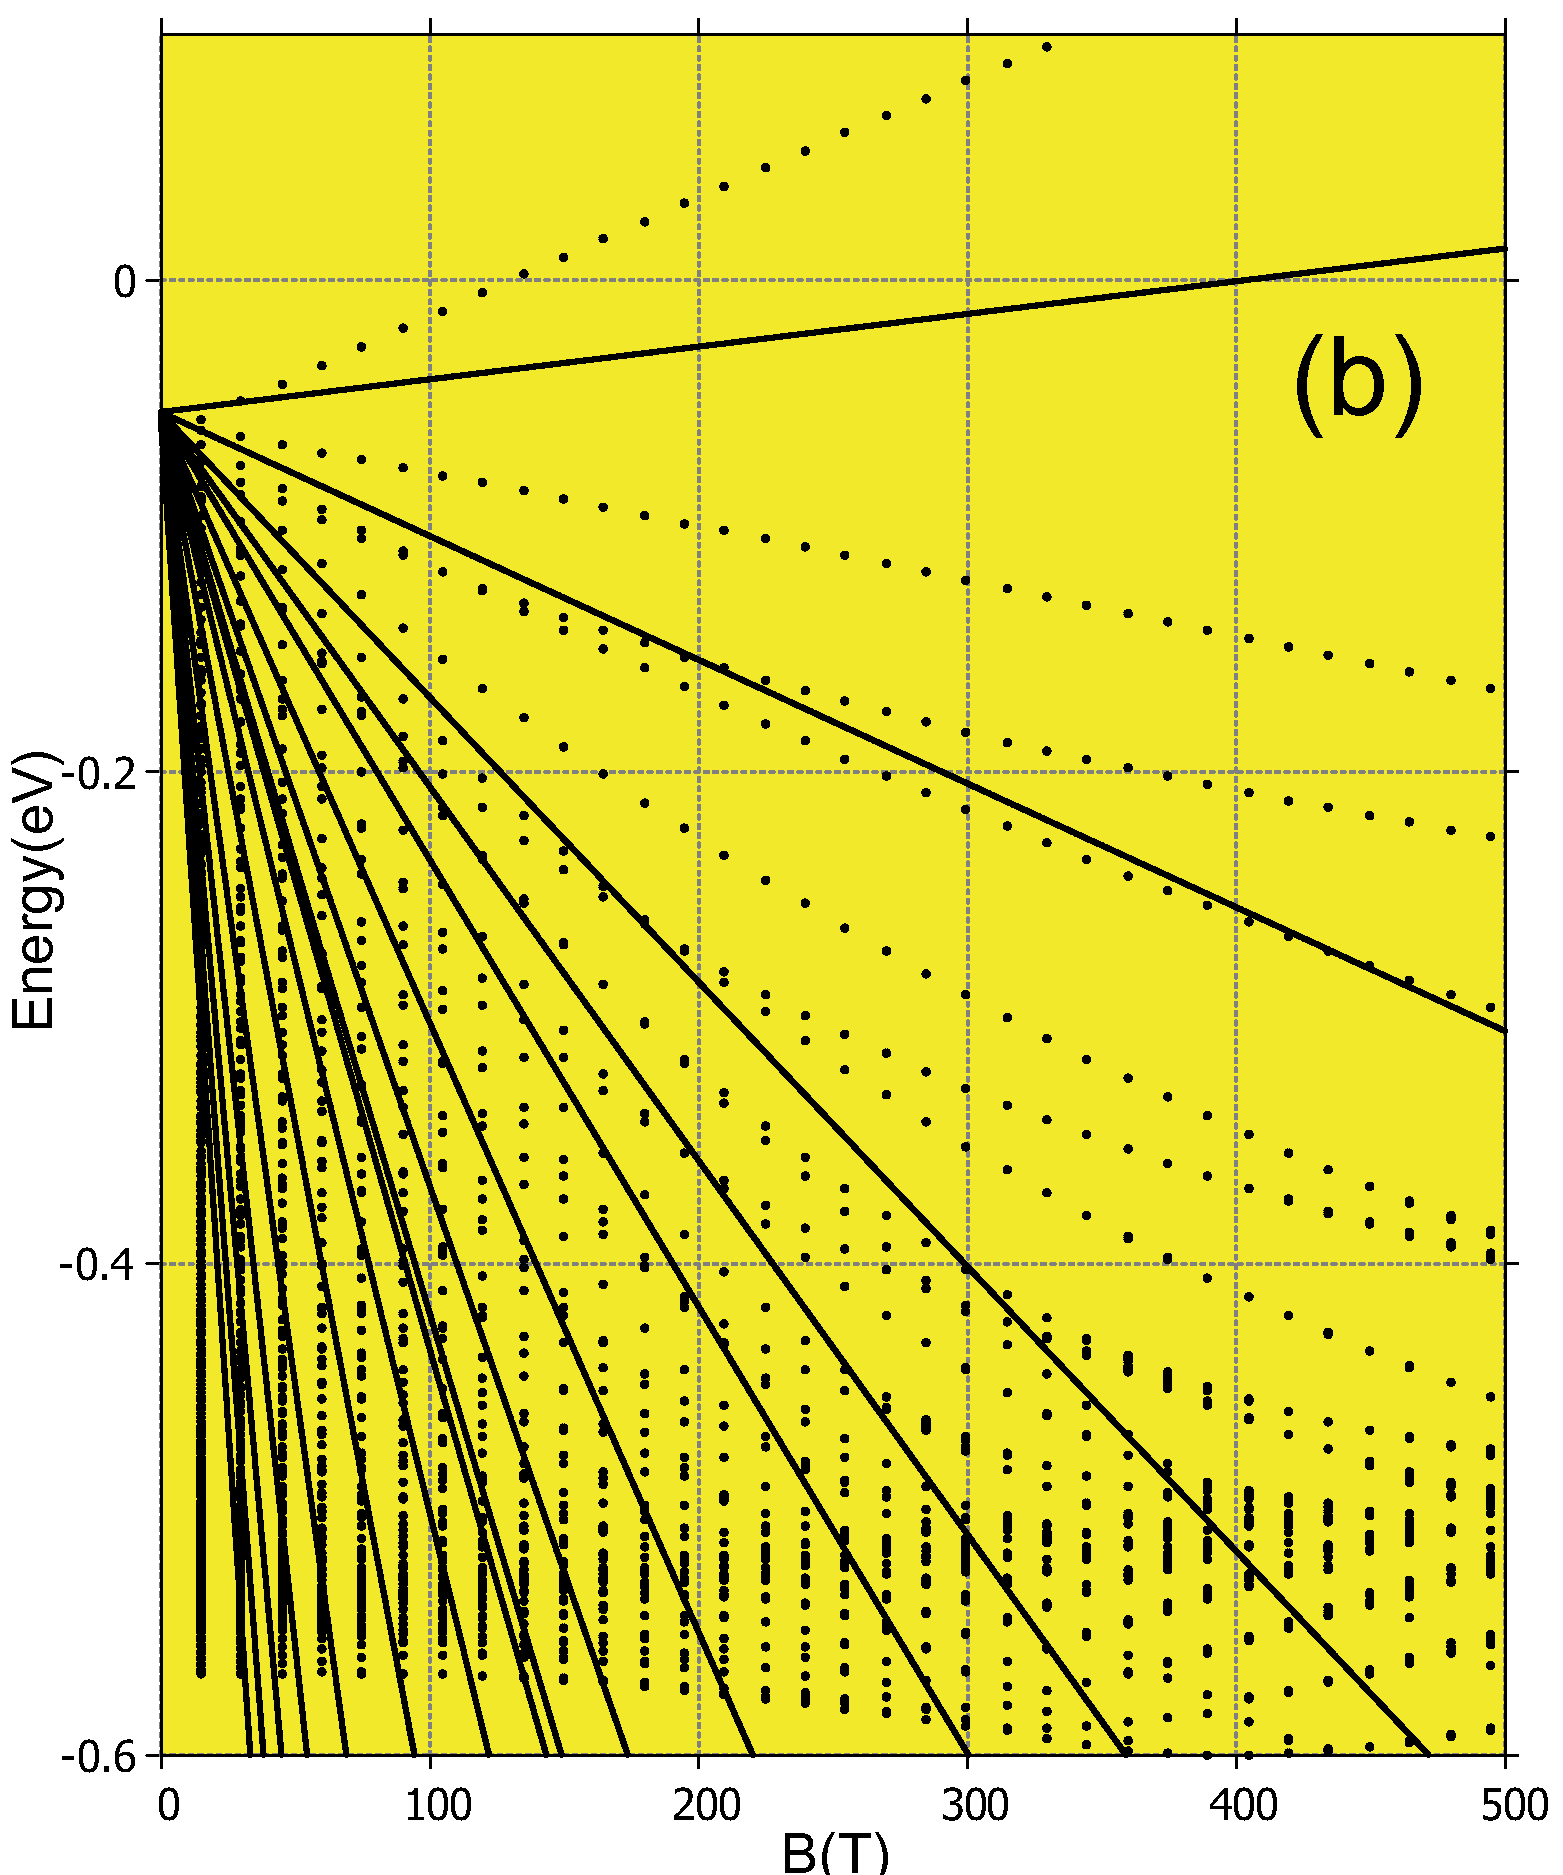
\includegraphics[width=0.85\textwidth,height=1.2\linewidth]{pic/landaulevel_3band_q_797_EF_final.pdf}
%	\end{subfigure}
%	\caption{
%		test
%	}
%\end{figure*}
%Ta có thể thấy một số mức Landau có năng lượng là được tăng tuyến tính theo cường độ từ trường, nhưng lại không cách đều và chính xác như hình của Hofstadter butterfly. Thêm vào đó có nhiều trạng thái mà năng lượng tại đó thì giảm trong khi đó thì từ trường lại tăng. những trạng thái này sẽ được gọi là những trạng thái ``kì cục'' mà ta sẽ bàn luận ở đây.\\
%Trong trường hợp một band, khối lượng hiệu dụng $m^{*}$ và điện tích là đủ để mô tả được phổ Landau theo sự thay đổi tuyến tính của từ trường. Trong trường hợp 2 band và 3 band thì


%It is this fan of Landau levels that responsible for the de Haas-van Alphen and Shubnikov-de Haas effects.

\section{Hall effect}
\subsection{The classical Hall effect}

Before delving into the quantum Hall effect, let us start by taking a look at its classical counterpart i.e., the Hall effect. The Hall effect arises when a conductor carrying an electric current is placed in an external magnetic field $\mathbf{B}$. The Lorentz force from the magnetic field causes the charges to accumulate on one side of the conductor. Starting with an electric field $\mathbf{E}$ established in the solid results in a current density $\mathbf{J}$ linearly related to the field through Ohm's law
\begin{gather}
	\mathbf{J} = \boldsymbol{\sigma} \mathbf{E}, \\
	\mathbf{E} = \sigma^{-1} \mathbf{J} = \rho \mathbf{J},
\end{gather}
where $\boldsymbol{\sigma}$ is the conductivity tensor and the resistivity $\mathbf{\rho}$ is defined as the inverse of the conductivity. This remains true when both are tensors
\begin{gather}
	\begin{pNiceMatrix}
		J_{x} \\
		J_{y}
	\end{pNiceMatrix}
	=
	\begin{pNiceMatrix}
		\sigma_{xx} & \sigma_{xy} \\
		\sigma_{yx} & \sigma_{yy} \\
	\end{pNiceMatrix}
	\begin{pNiceMatrix}
		E_{x} \\
		E_{y}
	\end{pNiceMatrix}, \\
	\begin{pNiceMatrix}
		E_{x} \\
		E_{y}
	\end{pNiceMatrix}
	%	=
	\begin{pNiceMatrix}
		\rho_{xx} & \rho_{xy} \\
		\rho_{yx} & \rho_{yy} \\
	\end{pNiceMatrix}
	\begin{pNiceMatrix}
		J_{x} \\
		J_{y}
	\end{pNiceMatrix}.
\end{gather}
The off-diagonal components of resistivity tensor is $\rho_{xy} = \rho_{yx} = \tfrac{B}{en}$. Usually we measure the resistance $R$, which differs from the resistivity $\rho$ by geometric factors. However, for $\rho_{xy}$, this thing coincide. To see this, consider a sample of material of length $L$ in the $y$-direction. We drop a voltage $V_{y}$ in the $y$-direction and measure the resulting current $I_{x}$ in the $x$-direction. The transverse resistance is
\begin{gather}
	R_{xy} = \frac{V_{y}}{I_{x}} = \frac{L E_{y}}{L J_{x}} = \frac{E_{y}}{J_{x}} = -\rho_{xy}.
\end{gather}
For a current $I_{x}$ flowing in the $x$-direction, and the corresponded electric field $E_{y}$ in the $y$-direction, the Hall coefficent is defined by
\begin{gather}
	R_{H} = \frac{\rho_{xy}}{B} = \frac{1}{en} ,
\end{gather}
showing the Hall resistance is a constant in the classical regime. We see that the Hall coefficent depends only on microscopic information about the material: the charge and density of conduction particles. The Hall coefficent does not depend on the scattering time $\tau$; it remains unaffected by the specific frictional mechanism present in the material.
\begin{figure*}[htb]
	\centering
	\begin{subfigure}[b]{0.495\textwidth}
		\centering
		{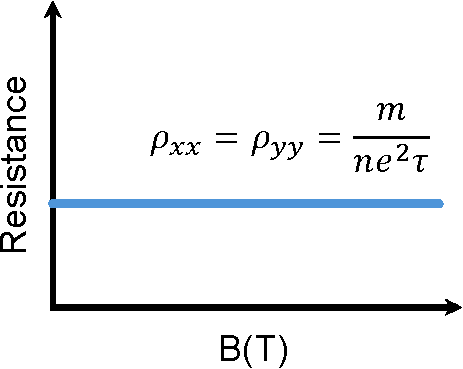
\includegraphics[width=0.75\linewidth]{pic/classRess.pdf}}
	\end{subfigure}
	\begin{subfigure}[b]{0.495\textwidth}
		\centering
		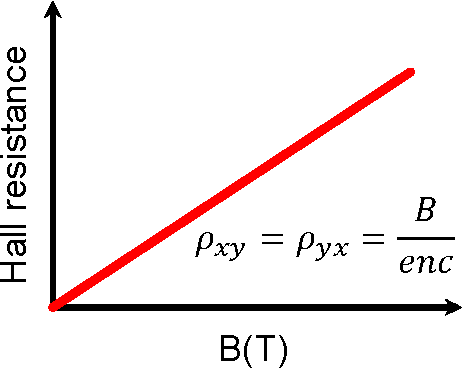
\includegraphics[width=0.75\linewidth]{pic/HallRess.pdf}
	\end{subfigure}
	\caption[Logitudinal resistance and Hall resistance plot.]{
		The longitudinal resistance on the right figure and the Hall resistance in the left figure. The graph shows both the longitudinal resistance and the Hall resistance is linear to the increasing magnetic field.
	}
\end{figure*}
\subsection{Berry curvature}
While the classical Hall effect is well explained by the Lorentz force deflecting charge carriers under a magnetic field, it fails to capture the quantized nature of Hall conductance observed in two-dimensional electron systems at low temperatures and high magnetic fields. This quantization is inherently quantum mechanical and cannot be described without considering the wavefunction topology of Bloch electrons.

In the semiclassical framework, the motion of electrons in a periodic potential acquires an additional term known as the anomalous velocity, which arises due to the Berry curvature of the Bloch bands. When an external electric field $\mathbf{E} = \left(E_{x}, E_{y}, 0\right)$ is applied, the crystal momentum $\mathbf{k}$ of the Bloch electrons become time-dependent, in accordance with the semiclassical acceleration theorem
\begin{gather}
	\hbar \dot{\mathbf{k}} = - e \mathbf{E}.
\end{gather}
The velocity of Bloch electrons is defined as
\begin{gather}
	\mathbf{v}_{\nu} = \frac{1}{\hbar} \nabla_{\mathbf{k}} \varepsilon_{\nu}(\mathbf{\mathbf{k}}) - \dot{\mathbf{k}} \times \Omega_{\nu}(\mathbf{k}),
\end{gather}
in which the second term, $ - \dot{\mathbf{k}} \times \Omega_{\nu}(\mathbf{k}) $, is known as the anomalous velocity. The Berry curvature $ \Omega_{\nu}(\mathbf{k}) $ of the $\nu$-th band is given by
\begin{gather}
	\Omega_{\nu}(\mathbf{k}) = \nabla_{\mathbf{k}} \times \Lambda_{\nu}(\mathbf{k}),
\end{gather}
where the Berry connection is defined as
\begin{gather}
	\Lambda_{\nu}(\mathbf{k}) = i \braket{u_{\nu,\mathbf{k}}}{\nabla_{\mathbf{k}} u_{\nu,\mathbf{k}}}.
\end{gather}

Substituting Eq.~(2.26) into Eq.~(2.27), we obtain the velocity for electrons of $\nu$-th band
\begin{gather}
	\mathbf{v}_{\nu}(\mathbf{k}) = \frac{1}{\hbar} \nabla_{\mathbf{k}} \varepsilon_{\nu} (\mathbf{k}) + \frac{e}{\hbar} \mathbf{E} \times \Omega_{\nu} (\mathbf{k}).
\end{gather}
The electric current density along the $x-$direction now is
\begin{equation}
	\begin{aligned}
		J_{x} &= \frac{1}{L^{2}} e \ev{v_{x}} \\
		&= \frac{e}{\hbar L^{2}} \sum_{n,\mathbf{k}} \frac{\partial \varepsilon_{n}(\mathbf{k})}{\partial k_{x}} f_{n}(\mathbf{k}) + \frac{e^{2}}{\hbar L^{2}} E_{y} \sum_{n,\mathbf{k}} \Omega_{\nu}^{z}(\mathbf{k}) f_{n}(\mathbf{k}).
	\end{aligned}
\end{equation}
Eq.~(2.31) allows us to express the Hall conductivity in terms of the Berry curvature integrated over all occupied states. This expression also implies that, if no subbands are occupied, the longitudinal conductivity vanishes, i.e., $\sigma_{xx} = 0$
\begin{gather}
	\sigma_{xy} = \f{e^{2}}{h} \sum_{n}^{\text{occ.}} \f{1}{2\pi} \dps\oiint_{\text{{BZ}}} d k_{x} d k_{y} \Omega_{\nu}^{z} (\mathbf{k}).
\end{gather}
The details derivation is given in \hyperref[appendix A]{Appendix A}.


\subsection{The Quantum Hall effect}
In Section~2.4.1, we arrived at the classical Hall resistance, which remains stable under the classical mechanics framework. However, our world is governed not only by classical physics but also by quantum mechanics. Things changes significantly at extremely low temperatures and strong magnetic fields, revealing new quantum phenomena.

There are two related phenomena which are associated to two different quantum Hall effects. These are called the \ac{IQHE} and \ac{FQHE}. In this study, we mainly focus on the \ac{IQHE} where the flux number and flux quanta are integers. This phenomenon can be understood without taking into account the Coulomb interaction between electrons, which means we shall continue using the single electron Hamiltonian that we described in \hyperref[Section 2.1]{Section 2.1}. In this section, we first discovered and subsequently understood theoretically the integer quantum Hall effect in the Hofstadter butterfly.

In two dimensional, there is a crucial relationship between the conductivity tensor $\boldsymbol{\sigma}$ and the resistivity tensor $\boldsymbol{\rho}$ is given by
\begin{equation}
	\begin{aligned}
		\begin{bmatrix}
			\sigma_{xx} & \sigma_{xy} \\
			\sigma_{yx} & \sigma_{yy}
		\end{bmatrix}
		\begin{bmatrix}
			\rho_{xx} & \rho_{xy} \\
			\rho_{yx} & \rho_{yy}
		\end{bmatrix}^{-1}
		=
		\f{1}{\rho_{xx} \rho_{yy} - \rho_{xy} \rho_{yx}}
		\begin{bmatrix}
			\rho_{yy}  & -\rho_{xy} \\
			-\rho_{yx} & \rho_{xx}
		\end{bmatrix}
	\end{aligned}.
\end{equation}
Let's take a look at the experimental data for the quantum Hall effect were perfomed in 1980 by von Klitzing \textit{et at.} \cite{klitzing90}
\begin{figure}[H]
	\centering
	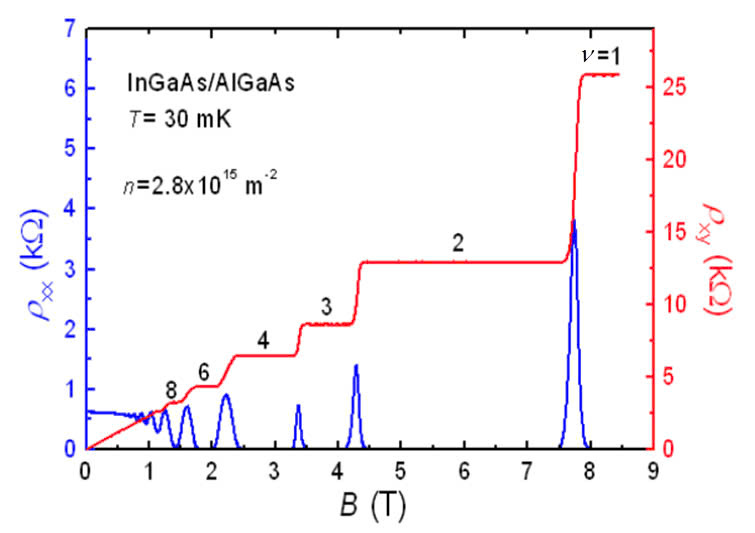
\includegraphics[width=0.7\linewidth]{pic/quantumhall.jpg}
	\caption[Quantum Hall effect by von Klitzing.]{This is the integer quantum Hall effect. For this Klaus von Klitzing was awarded the 1985 Nobel prize.}
\end{figure}
\noindent Both the Hall resistivity $\rho_{xy}$ and the longitudinal resistivity $\rho_{xx}$ depict fasinating behaviour. Perhaps the most striking feature in the figure is the fact that the Hall resistivity $\rho_{xy}$ sits on a plateau for a range of magnetic field, before jumping dramatically to the next plateau, while the longitudinal spikes sharply at the transistions between plateuax but vanishes on the plateaux themsleves. 

The Hall resistivity is now defined
\begin{gather}
	\rho_{xy} = \frac{R_{K}}{\nu}, \quad \nu = 1,2,...
\end{gather}
while $\nu$ is the total filled Landau levels and $R_{K}$ is Klitzing's resistance constant
\begin{gather}
	R_{K} = \frac{h}{e^{2}} = 25812.8074555 \Omega \pm 0.0000059 \Omega.
\end{gather}
Between two plateaux, if $\rho_{xy}  = 0$ then we get the familiar relation between resistivity and conductivity is $\sigma_{xx} = 1/\rho_{xx}$. But on these Hall plateaux
\begin{gather}
	\rho_{xy} = \rho_{yx} = \text{const} ,\; \rho_{xx} = \rho_{yy} = 0 ,
\end{gather}
this leads to
\begin{gather}
	\sigma_{xy} = \sigma_{yx} = 1 / \text{const} , \; \sigma_{xx} = \sigma_{yy} = 0.
\end{gather}
There is an apparent paradox here, we would call a system with $\rho_{xx} = 0$ is a perfect conductor, while one with $\sigma_{xx} = 0$ is a perfect insulator. But what if both $\rho_{xx} = 0$ and $\sigma_{xx} = 0$ occur simultaneously? A new material or a new state of matter?





%\subsection{Wannier diagram}
% a simplified replica of Fig, a powerful tool for visualizing the relationship between magnetic flux and electron filling in the system. Wannier's diagram provides a graphical representation of the allowed energy gaps in the Hofstadter spectruc as a function of the magnetic flux per unit cell and the electron filling factor. This diagram is particularly insightful because it captures the topological properties of the system through the distribution and behavior of these energy gaps.
%
%The fundamental of Wannier's diagram lies in the Diophantine gap equation
%\begin{gather}
%	\f{n}{n_{0}} = \nu \f{\Phi}{\Phi_{0}} + s,
%\end{gather}
%where $\frac{n}{n_{0}}$ is the electron filling factor, representing the ratio of the number of electrons per unit cell, $\nu$ is the Chern number associated with the quantized Hall conductance, and $s$ is another interg that corresponds to the gap index, effectively indicating the electron filling within the spectrum.
%
%
%
%The calculated Wannier's diagram, the energy density of state as a function of filling factor $\frac{n}{n_{0}}$ and magnetic flux $\Phi$ as illustrated in Fig, reveal the presence of these energy gaps across the spectrum. Each colored line in the diagram corresponds to an energy gap where the system exhibits an imcompressible quantumm Hall state, characterized by a quantized Hall conductance. The diagram not only provides a clear visualization of the gap structure but also offers insights into the topological phases that arise in monolayer TMD systems under varying magnetic flux conditions.
%\begin{figure}[H]
%	\centering
%	\includegraphics[width=0.8\textwidth,height=0.85\linewidth]{pic/wannier199.png}
%	\caption{Wannier diagram}
%\end{figure}

%\chapter{DISCUSSION}
%This
%\section{Result}
%\section{Discussion}

\chapter{\textbf{\uppercase{Three-band Tight-binding Model for TMDs}}}
In this chapter, based on the tight-binding framework introduced in Chapter~2, we adopt the model developed by Liu \textit{et al.}~\cite{PhysRevB.88.085433}, which constructs a minimal three-band model using three transistion metal orbitals as the basis. This model is commonly referred to as the three-band tight-binding model. Next, we extend this model to include the effects of an external magnetic field by using the Peierls substitution. Finally, we derive the Hamiltonian in the presence of the magnetic field.
\section{Three-band tight-binding model without magnetic field}\label{Section 3.1}

We take MoS$_2$ as a representative example and, based on previous \textit{ab initio} calculations, observe that at high-symmetry points in the Brillouin zone, specifically $\Gamma$, $K$, and $M$, the regions near the highest valence band and lowest conduction band are primarily contributed by the molybdenum $d_{z^2}$, $d_{xy}$, and $d_{x^2 - y^2}$ orbitals. In contrast, the $d_{xz}$, $d_{yz}$ orbitals of molybdenum and the $p_x$, $p_y$, and $p_z$ orbitals of sulfur contribute mainly to higher-energy subbands. This indicates that the low-energy bands near the band gap are predominantly governed by the $d_{z^2}$, $d_{xy}$, and $d_{x^2 - y^2}$ orbitals.  

Since only the orbitals of the M atom are included, we ignore the sum over atomic positions $\mathbf{r}_i$ within the unit cell in Eq.~(2.3), and denote the wave functions of the three orbitals of the M atom as
\begin{gather}
	\ket{\phi_{1}} = \ket{d_{z^{2}}} , \quad \ket{\phi_{2}} = \ket{d_{xy}} , \quad \ket{\phi_{3}} = \ket{d_{x^{2} - y^{2}}}.
\end{gather}
The Bloch wavefunction in this model has the form
\begin{gather}
	\psi_{\lambda,\mathbf{k}}(\mathbf{r}) = \sum_{j=1}^{3} C_{j}^{\lambda}(\mathbf{k}) \sum_{\mathbf{R}} e^{i \mathbf{k \cdot R}} \phi_{j}(\mathbf{r} - \mathbf{R}).
\end{gather}
The coefficents $C_{j}^{\lambda}(\mathbf{k})$ are the solutions of the eigenvalue equation
\begin{gather}
	\sum_{jj'}^{3} \left[H_{jj'}^{\text{TB}}(\mathbf{k}) - \varepsilon_{\lambda}(\mathbf{k}) S_{jj'}(\mathbf{k})\right] C_{j}^{\lambda}(\mathbf{k}) = 0,
\end{gather}
where
\begin{equation}
	\begin{aligned}
		H_{jj'}^{\text{TB}}(\mathbf{k}) = \sum_{\mathbf{R}} e^{i \mathbf{k \cdot R}} \bra{\phi_{j}(\mathbf{r})} \left[-\f{\hbar^{2} \nabla^{2}}{2m} + U_{0}(\mathbf{r})\right] \ket{\phi_{j'}(\mathbf{r - R})},
	\end{aligned}
\end{equation}
and
\begin{equation}
	\begin{aligned}
		S_{jj'}(\mathbf{k}) = \sum_{\mathbf{R}} \bra{\phi_{j}(\mathbf{r})} \ket{\phi_{j'}(\mathbf{r - R})} \approx \delta_{jj'}.
	\end{aligned}
\end{equation}

Take into account up to \ac{TNN} hopping, the matrix elements of the \ac{TB} Hamiltonian Eq.~(3.4) are
\begin{equation}
	\begin{aligned}
		H_{jj'}^{\text{TNN}}(\mathbf{k})
		& = \mathcal{E}_{jj'}(\mathbf{0}) + e^{i\mathbf{k}\cdot \mathbf{R}_{1}}\mathcal{E}_{jj'}(\mathbf{R}_{1}) + e^{i\mathbf{k}\cdot \mathbf{R}_{2}}\mathcal{E}_{jj'}(\mathbf{R}_{2}) + e^{i\mathbf{k}\cdot \mathbf{R}_{3}}\mathcal{E}_{jj'}(\mathbf{R}_{3})                 \\
		& + e^{i\mathbf{k}\cdot \mathbf{R}_{4}}\mathcal{E}_{jj'}(\mathbf{R}_{4}) + e^{i\mathbf{k}\cdot \mathbf{R}_{5}}\mathcal{E}_{jj'}(\mathbf{R}_{5}) + e^{i\mathbf{k}\cdot \mathbf{R}_{6}}\mathcal{E}_{jj'}(\mathbf{R}_{6})                                                 \\
		& + e^{i\mathbf{k}\cdot \tilde{\mathbf{R}}_{1}}\mathcal{E}_{jj'}(\tilde{\mathbf{R}}_{1}) + e^{i\mathbf{k}\cdot \tilde{\mathbf{R}}_{2}}\mathcal{E}_{jj'}(\tilde{\mathbf{R}}_{2}) + e^{i\mathbf{k}\cdot \tilde{\mathbf{R}}_{3}}\mathcal{E}_{jj'}(\tilde{\mathbf{R}}_{3}) \\
		& + e^{i\mathbf{k}\cdot \tilde{\mathbf{R}}_{}4}\mathcal{E}_{jj'}(\tilde{\mathbf{R}}_{4}) + e^{i\mathbf{k}\cdot \tilde{\mathbf{R}}_{5}}\mathcal{E}_{jj'}(\tilde{\mathbf{R}}_{5}) + e^{i\mathbf{k}\cdot \tilde{\mathbf{R}}_{6}}\mathcal{E}_{jj'}(\tilde{\mathbf{R}}_{6}) \\
		& + e^{i\mathbf{k}\cdot 2\mathbf{R}_{1}}\mathcal{E}_{jj'}(2\mathbf{R}_{1}) + e^{i\mathbf{k}\cdot 2\mathbf{R}_{2}}\mathcal{E}_{jj'}(2\mathbf{R}_{2}) + e^{i\mathbf{k}\cdot 2\mathbf{R}_{3}}\mathcal{E}_{jj'}(2\mathbf{R}_{3})                                           \\
		& + e^{i\mathbf{k}\cdot 2\mathbf{R}_{4}}\mathcal{E}_{jj'}(2\mathbf{R}_{4}) + e^{i\mathbf{k}\cdot 2\mathbf{R}_{5}}\mathcal{E}_{jj'}(2\mathbf{R}_{5}) + e^{i\mathbf{k}\cdot 2\mathbf{R}_{6}}\mathcal{E}_{jj'}(2\mathbf{R}_{6}) ,                                          \\
	\end{aligned}
\end{equation}
where
\begin{gather}
	\mathcal{E}_{jj'}(\mathbf{R}) = \bra{\phi_{j}(\mathbf{r})} \left[-\frac{\hbar \nabla^{2}}{2m} + U_{0} (\mathbf{r})\right] \ket{\phi_{j'}(\mathbf{r-R})},
\end{gather}
and $\mathbf{R}_{i}, \tilde{\mathbf{R}}_{i}$ and $2\mathbf{R}_{i}$ are one of the \ac{NN}, \ac{NNN} and third-nearest-neighbor (TNN) vectors, respectively, where $i = 1,...,6$, see in Fig.~3.1. In Table~3.1, we summarize the coordinates of hopping vectors considered in the model.
\begin{table}[h]
	\label{Table 2.1}
	\begin{equation*}
		\renewcommand{\arraystretch}{1.5}
		\begin{NiceArray}{c c c}
			\hline
			\hline
			\text{Vector}          & \text{Hopping relative coordinates} & \text{Cartesian's coordinates}                    \\
			\hline
			\mathbf{R}_{1}         & (m,n) \to (m+2,n)                   & a (1,0,0)                                         \\
			\mathbf{R}_{2}         & (m,n) \to (m+1,n-1)                 & a \left(\frac{1}{2},-\frac{\sqrt{3}}{2},0\right)  \\
			\mathbf{R}_{3}         & (m,n) \to (m-1,n-1)                 & a \left(-\frac{1}{2},-\frac{\sqrt{3}}{2},0\right) \\
			\mathbf{R}_{4}         & (m,n) \to (m-2,n)                   & a (-1,0,0)                                        \\
			\mathbf{R}_{5}         & (m,n) \to (m-1,n+1)                 & a \left(-\frac{1}{2},\frac{\sqrt{3}}{2},0\right)  \\
			\mathbf{R}_{6}         & (m,n) \to (m+1,n+1)                 & a \left(-\frac{1}{2},\frac{\sqrt{3}}{2},0\right)  \\
			\tilde{\mathbf{R}}_{1} & (m,n) \to (m+3,n-1)                 & l \left(\frac{\sqrt{3}}{2},-\frac{1}{2},0\right)  \\
			\tilde{\mathbf{R}}_{2} & (m,n) \to (m,n-2)                   & l \left(0,-1,0\right)                             \\
			\tilde{\mathbf{R}}_{3} & (m,n) \to (m-3,n-1)                 & l \left(-\frac{\sqrt{3}}{2},-\frac{1}{2},0\right) \\
			\tilde{\mathbf{R}}_{4} & (m,n) \to (m-3,n+1)                 & l \left(-\frac{\sqrt{3}}{2},\frac{1}{2},0\right)  \\
			\tilde{\mathbf{R}}_{5} & (m,n) \to (m,n+2)                   & l \left(0,-1,0\right)                             \\
			\tilde{\mathbf{R}}_{6} & (m,n) \to (m+3,n+1)                 & l \left(\frac{\sqrt{3}}{2},\frac{1}{2},0\right)   \\
			2\mathbf{R}_{1}        & (m,n) \to (m+4,n)                   & a (2,0,0)                                         \\
			2\mathbf{R}_{2}        & (m,n) \to (m+2,n-2)                 & a (1,-\sqrt{3},0)                                 \\
			2\mathbf{R}_{3}        & (m,n) \to (m-2,n-2)                 & a (-1,-\sqrt{3},0)                                \\
			2\mathbf{R}_{4}        & (m,n) \to (m-4,n)                   & a (-2,0,0)                                        \\
			2\mathbf{R}_{5}        & (m,n) \to (m-2,n+2)                 & a (-1,\sqrt{3},0)                                 \\
			2\mathbf{R}_{6}        & (m,n) \to (m+2,n+2)                 & a (1,\sqrt{3},0)                                  \\
			\hline
			\hline
		\end{NiceArray}
	\end{equation*}
	\caption[Coordinates relative of hopping terms.]{Hopping vectors used in the model and their hopping respective relative coordinates to the original site $(m,n)$, where $a = 3.190$ \AA \;is lattice constant and $l = a\sqrt{3}$.}
\end{table}
%\begin{equation}
%\begin{aligned}
%	\mathbf{R}_{1} & = (a,0), \quad \mathbf{R}_{2} = \left(\f{a}{2}, - \f{a\sqrt{3}}{2}\right), \quad \mathbf{R}_{3} = \left(-\f{a}{2},-\f{a\sqrt{3}}{2}\right), \\
%	\mathbf{R}_{4} & = (-a,0), \quad \mathbf{R}_{5} = \left(-\f{a}{2}, \f{a\sqrt{3}}{2}\right), \quad \mathbf{R}_{6} = \left(\f{a}{2},\f{a\sqrt{3}}{2}\right).
%\end{aligned}
%\end{equation}
%Here, $\mathbf{R}_{1-6}$ are the positions of the nearest neighbors M atoms, see Fig. 2.1
\begin{figure}[H]
	\centering
	\includegraphics[width=\linewidth]{pic/schematicLatticeTNN.pdf}
	\caption[The hexagonal structure with neighbor hoppings.]{\label{fig:Lattice vectors}The hexagonal structure of the monolayer \ac{TMD} with the metal atoms at the green larger circles and the chalcogen atoms at the smaller yellow circles. The solid red, dash blue and dot purple arrows prepresent the \ac{NN} ($\mathbf{R}_{i}$), \ac{NNN} ($\tilde{\mathbf{R}}_{i}$) and \ac{TNN} (2$\mathbf{R}_{i}$), respectively, and $\mathbf{R}$ are lattice vectors, where $i = 1,...,6$.}
\end{figure}
%%%%% Table
\begin{table}[h]
	\begin{equation*}
		\renewcommand{\arraystretch}{1.5}
		\begin{NiceArray}{c c c c c c c}
			\hline
			\hline
			g_{n}                  & x'                                   & y'                                  & z' & z'^{2} & x'y'                                               & \frac{1}{2}(x'^{2} - y'^{2})                        \\
			\hline
			E                      & x                                    & y                                   & z  & z^{2}  & xy                                                 & \frac{1}{2}(x^{2} - y^{2})                          \\
			C_{3}(\frac{-2\pi}{3}) & -\frac{1}{2}x + \frac{\sqrt{3}}{2} y & -\frac{\sqrt{3}}{2}x - \frac{1}{2}y & z  & z^{2}  & -\frac{1}{2}xy + \frac{\sqrt{3}}{4}(x^{2} + y^{2}) & -\frac{\sqrt{3}}{2} xy - \frac{1}{4}(x^{2} - y^{2}) \\
			C_{3}(\frac{-4\pi}{3}) & -\frac{1}{2}x - \frac{\sqrt{3}}{2} y & \frac{\sqrt{3}}{2}x + \frac{1}{2}y  & z  & z^{2}  & -\frac{1}{2}xy - \frac{\sqrt{3}}{4}(x^{2} + y^{2}) & \frac{\sqrt{3}}{2} xy - \frac{1}{4}(x^{2} - y^{2})  \\
			C_{2}(-\pi)            & -x                                   & -y                                  & z  & z^{2}  & xy                                                 & \tfrac{1}{2}(x^{2} - y^{2})                         \\
			\sigma_{\nu}           & -x                                   & y                                   & z  & z^{2}  & -xy                                                & \frac{1}{2}(x^{2} - y^{2})                          \\
			\sigma'_{\nu}          & \frac{1}{2}x - \frac{\sqrt{3}}{2}    & -\frac{\sqrt{3}}{2}x - \frac{1}{2}y & z  & z^{2}  & \frac{1}{2}xy - \frac{\sqrt{3}}{4}(x^{2} + y^{2})  & -\frac{\sqrt{3}}{2} xy - \frac{1}{4}(x^{2} - y^{2}) \\
			\sigma''_{\nu}         & \frac{1}{2}x + \frac{\sqrt{3}}{2}    & \frac{\sqrt{3}}{2}x - \frac{1}{2}y  & z  & z^{2}  & \frac{1}{2}xy + \frac{\sqrt{3}}{4}(x^{2} + y^{2})  & \frac{\sqrt{3}}{2} xy - \frac{1}{4}(x^{2} - y^{2})  \\
			\hline
			\hline
		\end{NiceArray}
	\end{equation*}
	\caption[Symmetry operators of the $D_{3h}$ point group.]{Some symmetry operators of the $D_{3h}$ point group on basis functions taking $(x,y,z)$ into $(x',y',z')$. $C_{3}(\frac{-2\pi}{3})$ and $C_{3}(\frac{-4\pi}{3})$ are the rotaions by $\frac{-2\pi}{3}$ and $\frac{-4\pi}{3}$ around the $z$ axis, respectively. $\sigma_{\nu}$ is the reflection angular bisector of $R_{1}$ and $R_{6}$ in Fig. 2.1, and $\sigma'_{\nu},\sigma''_{\nu}$ are obtained through rotating $\sigma_{\nu}$ around the $z$ axis by $2\pi/3$ and $4\pi/3$, respectively.}
\end{table}
%%%%%%%%

One parameterizes the matrices $\mathcal{E}(\mathbf{0}), \mathcal{E}(\mathbf{R}_{1}),\mathcal{E}(\mathbf{\tilde{\mathbf{R}}}_{1}) , \mathcal{E}(\mathbf{\tilde{\mathbf{R}}}_{4})$ and $ \mathcal{E}(2\mathbf{R}_{1})$ by
\begin{equation}
	\renewcommand{\arraystretch}{0.7}
	\begin{aligned}
		\mathcal{E}(\mathbf{0})
		& =
		\begin{pNiceMatrix}
			\epsilon_{1} & 0            & 0            \\
			0            & \epsilon_{2} & 0            \\
			0            & 0            & \epsilon_{2}
		\end{pNiceMatrix},
		\mathcal{E}(\mathbf{R}_{1})
		=
		\begin{pNiceMatrix}
			t_{0}  & t_{1}   & t_{2}  \\
			-t_{1} & t_{11}  & t_{12} \\
			t_{2}  & -t_{12} & t_{22}
		\end{pNiceMatrix},
		\mathcal{E}(2\mathbf{R}_{1})
		=
		\begin{pNiceMatrix}
			u_{0}  & u_{1}   & u_{2}  \\
			-u_{1} & u_{11}  & u_{12} \\
			u_{2}  & -u_{12} & u_{22}
		\end{pNiceMatrix}, \\
		\mathcal{E}(\tilde{\mathbf{R}}_{1})
		& =
		\begin{pNiceMatrix}
			r_{0}                   & r_{1}  & -\frac{r_{1}}{\sqrt{3}}            \\
			r_{2}                   & r_{11} & r_{12}                             \\
			-\frac{r_{2}}{\sqrt{3}} & r_{12} & r_{11} + \frac{2\sqrt{3}}{3}r_{12}
		\end{pNiceMatrix},
		\mathcal{E}(\tilde{\mathbf{R}}_{4}) = \mathcal{E}(\tilde{\mathbf{R}}_{1})^{\text{T}}
		=
		\begin{pNiceMatrix}
			r_{0}                   & r_{2}  & -\frac{r_{2}}{\sqrt{3}}            \\
			r_{1}                   & r_{11} & r_{12}                             \\
			-\frac{r_{1}}{\sqrt{3}} & r_{12} & r_{11} + \frac{2\sqrt{3}}{3}r_{12}
		\end{pNiceMatrix}.
	\end{aligned}
\end{equation}
Given $\mathcal{E}(\mathbf{R}_{1}),\mathcal{E}(2\mathbf{R}_{1}),\mathcal{E}(\tilde{\mathbf{R}}_{1}),\mathcal{E}(\tilde{\mathbf{R}}_{4})$, the matrix $\mathcal{E}(\mathbf{R}_{i})$ corresponding to all neighbor sites $\mathbf{R}_{i}$ can be generated by
\begin{gather}
	\mathcal{E}(g_{n} \mathbf{R}) = D(g_{n}) \mathcal{E} (\mathbf{R}) D^{\dagger}(g_{n}),
\end{gather}
where $D(g_{n})$ is the matrix of the irreducible representation, $g_{n}$ are symmetry operators of $D_{3h}$ point groups, $\{E,2 C_3, 3C_2, 2S_3,\sigma_{h},3\sigma_{\nu}\}$,
%Particularly, we have $\mathcal{E}(\mathbf{R}_{2}) = \mathcal{E}(\sigma'_{\nu}\mathbf{R}_{1})$, $\mathcal{E}(\mathbf{R}_{3}) = \mathcal{E}(C_{3}(-\frac{2\pi}{3})\mathbf{R}_{1})$,
%$\mathcal{E}(\mathbf{R}_{4}) = \mathcal{E}(\sigma_{\nu}\mathbf{R}_{1})$, $\mathcal{E}(\mathbf{R}_{5}) = \mathcal{E}(C_{3}(-\frac{4\pi}{3}\mathbf{R}_{1})$,
%$\mathcal{E}(\mathbf{R}_{6}) = \mathcal{E}(\sigma''_{\nu}\mathbf{R}_{1})$.
see in \hyperref[appendix B]{Appendix B} for more details about the calculation. Table 2.2 depicts the transformation of the basis functions under the action of symmetry operators. Also, from Table 3.2, we obtain irreducible matrices as follows
\begin{equation}
	\renewcommand{\arraystretch}{0.8}
	\begin{aligned}
		& D(C_{3}(-\tfrac{2\pi}{3}))
		=
		\begin{pNiceMatrix}
			1 & 0           & 0          \\
			0 & -1/2        & \sqrt{3}/2 \\
			0 & -\sqrt{3}/2 & -1/2
		\end{pNiceMatrix},
		\quad D(C_{3}(-\tfrac{4\pi}{3}))
		=
		\begin{pNiceMatrix}
			1 & 0          & 0            \\
			0 & -1/2       & - \sqrt{3}/2 \\
			0 & \sqrt{3}/2 & -1/2
		\end{pNiceMatrix}, \\
		& D(\sigma_{\nu})
		=
		\begin{pNiceMatrix}
			1 & 0  & 0 \\
			0 & -1 & 0 \\
			0 & 0  & 1
		\end{pNiceMatrix},
		\quad D(\sigma'_{\nu})
		=
		\begin{pNiceMatrix}
			1 & 0           & 0           \\
			0 & 1/2         & -\sqrt{3}/2 \\
			0 & -\sqrt{3}/2 & -1/2
		\end{pNiceMatrix}, \\
		& D(\sigma''_{\nu})
		=
		\begin{pNiceMatrix}
			1 & 0          & 0          \\
			0 & 1/2        & \sqrt{3}/2 \\
			0 & \sqrt{3}/2 & -1/2
		\end{pNiceMatrix}.
	\end{aligned}
\end{equation}
The remaining hopping matrices can be obtained by applying the $C_{3}$ rotation, mirror, and relation $\mathcal{E}(-\mathbf{R}) = \mathcal{E}(\mathbf{R})^{\text{T}}$. Therefore, we have the hopping terms for three-band \ac{TBM} including \ac{TNN} are given in \hyperref[appendix B]{Appendix B}.

The \ac{TNN} tight-binding Hamiltonian now can be written as
\begin{equation}
	\renewcommand{\arraystretch}{0.85}
	\begin{aligned}
		H^{\text{TNN}}(\mathbf{k})
		=
		\begin{pNiceMatrix}
			V_{0}     & V_{1}      & V_{2}  \\
			V_{1}^{*} & V_{11}     & V_{12} \\
			V_{2}^{*} & V_{12}^{*} & V_{22}
		\end{pNiceMatrix},
	\end{aligned}
\end{equation}
where
\begin{equation}
	\begin{aligned}
		V_0         & = \epsilon_1 + 2t_0 (2\cos\alpha\cos\beta + \cos2\alpha) + 2r_0 (2\cos3\alpha\cos\beta+\cos2\beta),                                       \\
		\Re[V_1]    & = -2\sqrt{3}t_2 \sin \alpha \sin \beta + 2(r_1 + r_2)\sin 3 \alpha \sin \beta - 2\sqrt{3} u_2 \sin 2\alpha \sin 2\beta,                      \\
		\Im[V_1]    & = 2 t_1 \sin \alpha (2 \cos \alpha +\cos \beta) + 2(r_1 - r_2) \sin 3\alpha \cos \beta + 2u_1 \sin 2\alpha (2\cos 2\alpha + \cos 2\beta)     \\
		\Re[V_2]    & = 2t_2 (\cos 2\alpha - \cos \alpha \cos \beta) -\frac{2}{\sqrt{3}} (r_1 + r_2 ) (\cos 3\alpha \cos \beta - \cos 2 \beta)                     \\&\quad + 2u_2 (\cos 4\alpha -\cos 2\alpha \cos 2\beta),\\
		\Im[V_2]    & = 2\sqrt{3} t_1 \cos \alpha \sin \beta +\frac{2}{\sqrt{3}} \sin \beta (r_1 -r_2 )(\cos 3\alpha + 2\cos \beta),                               \\
		V_{11}      & = \epsilon_2 + (t_{11}+3t_{22})\cos \alpha \cos \beta + 2 t_{11} \cos 2\alpha + 4r_{11} \cos 3\alpha \cos \beta                           \\ &\quad +2 (r_{11} + \sqrt{3} r_{12}) \cos 2\beta + (u_{11} + 3 u_{22})\cos 2 \alpha \cos 2\beta + 2 u_{11} \cos 4\alpha,\\
		\Re[V_{12}] & = \sqrt{3} (t_{22} - t_{11}) \sin \alpha \sin \beta +4 r_{12} \sin 3\alpha \sin \beta + \sqrt{3} (u_{22} - u_{11}) \sin 2\alpha \sin 2\beta, \\
		\Im[V_{12}] & = 4 t_{12} \sin \alpha (\cos \alpha -\cos \beta) + 4u_{12} \sin 2\alpha (\cos 2\alpha - \cos 2\beta),                                        \\
		V_{22}      & = \epsilon_2 +(3t_{11} + t_{22}) \cos \alpha \cos \beta + 2 t_{22} \cos 2 \alpha + 2 r_{11}(2\cos 3\alpha \cos \beta + \cos 2 \beta)      \\&\quad + \frac{2}{\sqrt{3}} r_{12} (4\cos 3\alpha \cos \beta - \cos 2\beta) + (3 u_{11} + u_{22}) \cos 2\alpha \cos 2\beta + 2u_{22} \cos 4\alpha,
	\end{aligned}
\end{equation}
\begin{equation}
	\begin{aligned}
		(\alpha,\beta) = \left(\frac{1}{2}k_{x}a,\frac{\sqrt{3}}{2}k_{y}a\right).
	\end{aligned}
\end{equation}

The nineteen tight-binding parameters shown in \hyperref[B.2]{Table B.2} are determined by fitting to the band structure obtained from \textit{ab initio} calculations.

%By substituting Eq.~2.19 into Eq.~2.11, we derive the eigenvalues of the Hamiltonian. These are computed over all $k$-points throughout the entire \ac{BZ}, and the corresponding band structure is illustrated in Fig.~2.3. The presence of three orbitals from the M atom in the unit cell results in three energy bands: one \ac{VB} and two \acp{CB}.

%\begin{figure*}[htb]
%	\centering
%	\includegraphics[width=0.7\linewidth]{pic/bandstructureTNN.pdf}
%	\caption[Band structure of $\mathrm{MoS}_2$ material along $\Gamma$-K direction]{\label{band structure} The band structure of monolayer MoS$_{2}$ along $\Gamma$-K direction using (LDA) fitting parameters.}
%\end{figure*}

Due to the significant mass of the transition-metal atom M, its \ac{SOC} can be large. For simplicity, we consider only the on-site contribution, which corresponds to the $\mathbf{L \cdot S}$ term originating from the $M$ atoms. Using the basis set $\left\{\ket{d_{z^{2}},\uparrow},\ket{d_{xy},\uparrow},\ket{d_{x^{2} - y^{2}},\uparrow},\ket{d_{z^{2}},\downarrow},\ket{d_{xy},\downarrow},\ket{d_{x^{2} - y^{2}},\downarrow}\right\}$, we derive the SOC term in the Hamiltonian as
\begin{gather}
	H{'}
	= \lambda \mathbf{L \cdot S}
	= \f{\lambda}{2}
	\begin{pNiceMatrix}
		L_{z}           & L_{x} - i L_{y} \\
		L_{x} + i L_{y} & -L_{z}
	\end{pNiceMatrix},
\end{gather}
in which
\begin{gather}
	L_{z}
	=
	\begin{pNiceMatrix}
		0 & 0   & 0  \\
		0 & 0   & 2i \\
		0 & -2i & 0
	\end{pNiceMatrix},
\end{gather}
is the matrix of $\hat{L}_{z}$ ($z$ component of the orbital angular momentum) in bases of $d_{z^{2}},d_{xy},d_{x^{2} - y^{2}}$ and $\lambda$ is characterized the strength of the \ac{SOC}. Noting that, under the three bases, the matrix elements of $\hat{L}_{x}$ and $\hat{L}_{y}$ are all zeros. Therefore the full \ac{TB} Hamiltonian for the magnetic unit cell with the SOC as follows
\begin{equation}
	\begin{aligned}
		H_{\text{SOC}}(\mathbf{k})
		& = \mathbf{I}_{2} \otimes H^{TNN}(\mathbf{k}) + H{'} \\
		& =
		\begin{pmatrix}
			H_{3 \times 3}(\mathbf{k}) + \frac{\lambda}{2} L_{z} & 0                                                      \\
			0                                                      & H_{3 \times 3}(\mathbf{k}) - \frac{\lambda}{2} L_{z}
		\end{pmatrix},
	\end{aligned}
\end{equation}
in which $\mathbf{I}_{2}$ is the $2\times 2$ identity matrix.
% and $\mathbf{I}_{q}$ is the $q\times q$.
%\begin{figure*}[htb]
%	\begin{subfigure}[b]{0.495\textwidth}
%		\centering
%		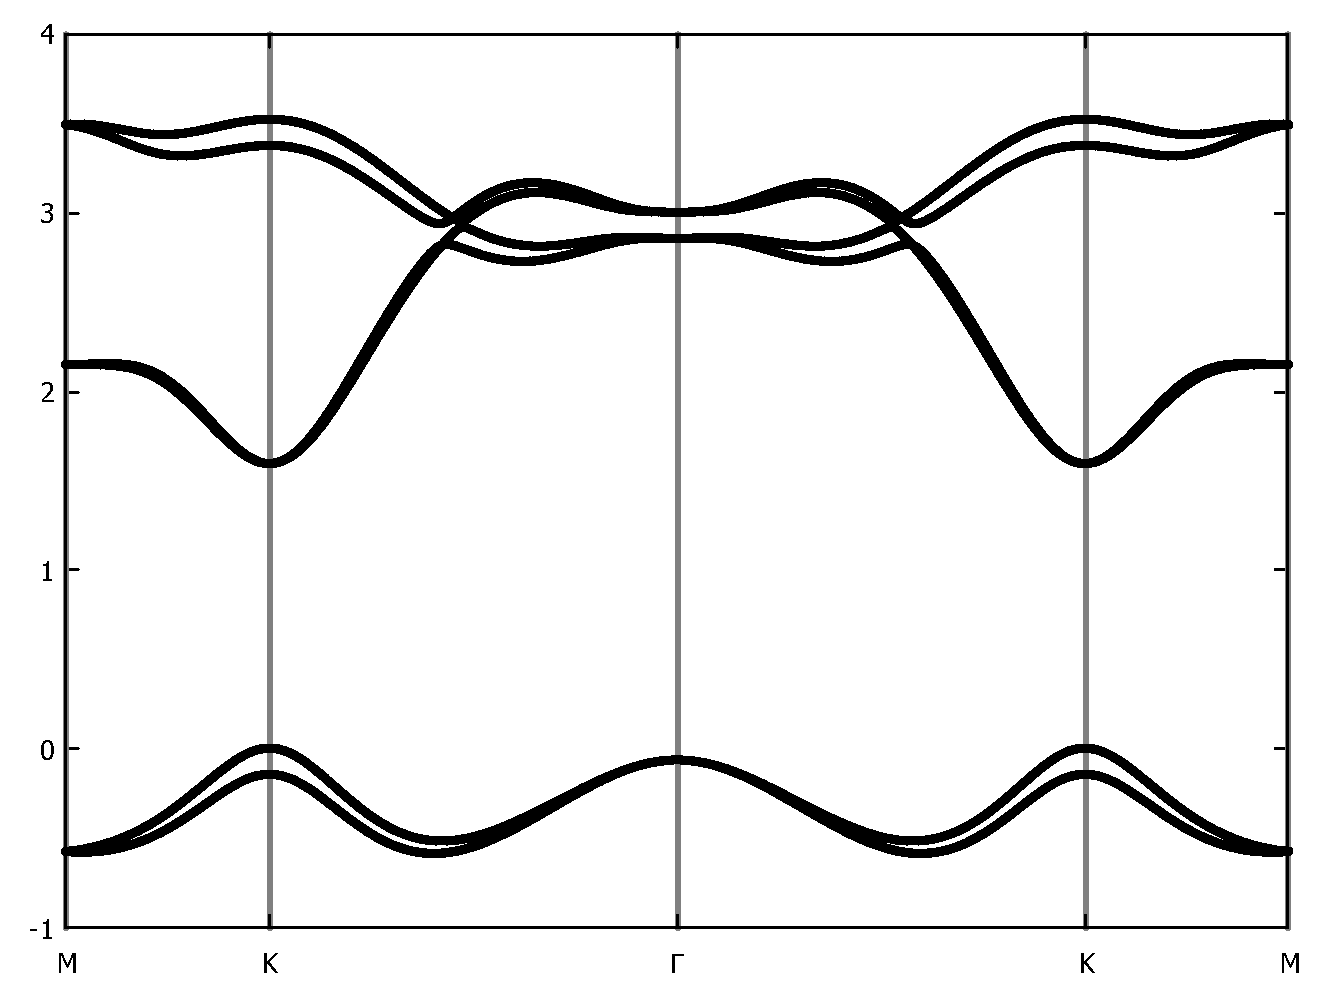
\includegraphics[width=\linewidth]{pic/bandstructureSOC.pdf}
%		%\caption{\label{band structure SOC}}
%	\end{subfigure}
%	\begin{subfigure}[b]{0.495\textwidth}
%		\centering
%		\includegraphics[width=\linewidth]{pic/bandstructureSOCTNN.pdf}
%		%\caption{\label{HB SOC}}
%	\end{subfigure}
%	\caption[Banstructure of NN and TNN monolayer MoS$_{2}$ with SOC without magnetic field.]{The band structure of monolayer MoS$_2$ in the absence of a magnetic field along the $\Gamma$–K direction exhibits significant spin splittings at the $K$ and $-K$ points, primarily due to spin–orbit coupling (SOC). Figures 2.8(a) and 2.8(b) show the results obtained using \ac{NN} and \ac{TNN} model, respectively.
%	}
%\end{figure*}
%The diagram in Fig. 2.8 shows the significant splitting of the valence bands at the $K$ and $K'$ points of MoS$_{2}$, caused by the \ac{SOC}, with a value of $\Delta_{\text{SOC}}^{\lambda} = 2 \lambda = 146$ meV. Although the \ac{NN} \ac{TB} model is not accurate as the TNN one, it can be seen that the \ac{NN} \ac{TB} bands agree well the \ac{TNN} results near the $K$ and $K'$ points.


\section{Three-band tight binding model under a magnetic field}\label{Section 3.2}
Under an uniform magnetic field given by a vector potential $\mathbf{A}(\mathbf{r})$ the single electron Hamiltonian changes into
\begin{gather}
	H = \f{\left(-i\hbar \boldsymbol{\nabla} + e \mathbf{A(r)}\right)^{2}}{2m} + U_{0}(\mathbf{r}) + g^{*} \mu_{B} \mathbf{B} \cdot \mathbf{L},
\end{gather}
where $\mu_{B} = \f{e\hbar}{2m}$ is Bohr magneton, $g^{*}$ is an effective Landé g-factor, $\mathbf{B} = \boldsymbol{\nabla} \times  \mathbf{A}$ is the uniform magnetic field, and $\mathbf{L}$ is the angular momentum. It is possible to add a phase factor to the tight-binding wavefunction
\begin{gather}
	\psi_{\lambda,\mathbf{k}} (\mathbf{r}) = \sum_{j=1}^{3} C_{j}^{\lambda}(\mathbf{k}) \sum_{\mathbf{R}} e^{i\mathbf{k \cdot R}} e^{ \theta_{\mathbf{R}}(\mathbf{r})} \phi_{j}(\mathbf{r} - \mathbf{R}).
\end{gather}
We now have
\begin{equation}
	\begin{aligned}
		H_{j j'} (\mathbf{k}) = H_{jj'}^{\text{TB}}(\mathbf{k}) + H_{jj'}^{Z}(\mathbf{k}),
	\end{aligned}
\end{equation}
where
\begin{equation}
	\begin{aligned}
		H_{jj'}^{\text{TB}}(\mathbf{k})
		& = \sum_{\mathbf{R}} \bra{\phi_{j}(\mathbf{r})} e^{-i \theta_{\mathbf{0}}(\mathbf{r})} \left[\f{(-i\hbar \boldsymbol{\nabla} + e \mathbf{A}(\mathbf{r}))^{2}}{2m} + U_{0}(\mathbf{r}) \right] e^{i\mathbf{k \cdot R}} e^{ \theta_{\mathbf{R}}(\mathbf{r})} \ket{\phi_{j'}(\mathbf{r - R})}                        \\
		& = \sum_{\mathbf{R}} \bra{\phi_{j}(\mathbf{r})} e^{i(\mathbf{k \cdot R} +\theta_{\mathbf{R}} - \theta_{\mathbf{0}} )} \left[ \f{ \left( -i\hbar \boldsymbol{\nabla} + e \mathbf{A} + \hbar \boldsymbol{\nabla} \theta_{\mathbf{R}} \right)^{2} }{2m} + U_{0}(\mathbf{r}) \right] \ket{\phi_{j'}(\mathbf{r - R})}.
	\end{aligned}
\end{equation}
Since the Zeeman interaction orginates from the coupling between the magnetic field and the orbital angular momentum of electrons localized at atomic sites, it is an on-site effect rather than a hopping term. Therefore, the Hamiltonian Zeeman is approximated by keeping only $\mathbf{R} = 0$ contribution
\begin{equation}
	\begin{aligned}
		H_{jj'}^{Z}(\mathbf{k})
		& = g^{*} \mu_{B} \mathbf{B} \cdot \sum_{\mathbf{R}} \bra{\phi_{j}(\mathbf{r})} e^{i(\mathbf{k \cdot R} + \theta_{\mathbf{R}} - \theta_{\mathbf{0}} )} \mathbf{L} \ket{\phi_{j'}(\mathbf{r - R})} \\
		& \approx g^{*} \mu_{B} \mathbf{B} \cdot \sum_{\mathbf{R}} \bra{\phi_{j}(\mathbf{r})} \mathbf{L} \ket{\phi_{j'}(\mathbf{r})}.
	\end{aligned}
\end{equation}
By choosing $\theta_{\mathbf{R}} = - \f{e}{\hbar} \int_{\mathbf{R}}^{\mathbf{r}} \mathbf{A(\mathbf{r'})} \cdot d\mathbf{r'}$ as Peierls substitution \cite{peierls1933theorie}, the Hamiltonian in Eq.~(3.20) now reads
\begin{equation}
	\begin{aligned}
		H_{jj'}^{\text{TB}}(\mathbf{k})
		& = \sum_{\mathbf{R}} \bra{\phi_{j}(\mathbf{r})} e^{i\mathbf{k \cdot R} - \frac{ie}{\hbar} \int_{\mathbf{R}}^{\mathbf{r}} \mathbf{A}(\mathbf{r'}) \cdot d\mathbf{r'} + \frac{ie}{\hbar}\int_{\mathbf{0}}^{\mathbf{r}}\mathbf{A(\mathbf{r'})}\cdot d\mathbf{r'} } \left[- \f{\hbar^{2} \boldsymbol{\nabla}^{2}}{2m} + U_{0} (\mathbf{r}) \right] \ket{\phi_{j'}(\mathbf{r - R})} \\
		& = \sum_{\mathbf{R}}  e^{i\mathbf{k \cdot R}} e^{\frac{ie}{\hbar} \int_{\mathbf{0}}^{\mathbf{R}} \mathbf{A(\mathbf{r'})} \cdot d \mathbf{r'} } \bra{\phi_{j}(\mathbf{r})} e^{-\frac{ie}{\hbar} \Phi_{\mathbf{R,r,0}}} \left[ -\f{\hbar^{2} \boldsymbol{\nabla}^{2}}{2m} + U_{0} (\mathbf{r}) \right] \ket{\phi_{j'}(\mathbf{r - R})},
	\end{aligned}
\end{equation}
where $\Phi_{\mathbf{R,r,0}} = \oint_{\mathbf{R,r,0}} \mathbf{A(\mathbf{r'})} \cdot d\mathbf{r'} $ is the closed loop line integral of $\mathbf{A}$ along the triangle points $\mathbf{R,r,0}$, and $\int_{\mathbf{0}}^{\mathbf{R}} \mathbf{A(\mathbf{r'})} \cdot d \mathbf{r'}$ is the path integral along the two points $\mathbf{R,0}$. Besides that, we have used the fact that
\begin{align}
	\int_{\mathbf{R}}^{\mathbf{r}} \mathbf{A(\mathbf{r'})} \cdot d\mathbf{r'} + \int_{\mathbf{r}}^{\mathbf{0}} \mathbf{A(r')} \cdot d\mathbf{r'} = \Phi_{\mathbf{R,r,0}} - \int_{\mathbf{0}}^{\mathbf{R}} \mathbf{A(\mathbf{r'})} \cdot d \mathbf{r'}.
\end{align}
We can show that the flux term $\Phi_{\mathbf{R}, \mathbf{r}, \mathbf{0}}$ is negligibly small based on two observations~\cite{yalcin_2019}. Firstly, when $\mathbf{r}$ is far from the lattice points $\mathbf{R}$ and $\mathbf{0}$, the enclosed flux may be large. However, since the atomic orbitals are highly localized at these two lattice sites, the corresponding hopping amplitude becomes vanishingly small, effectively suppressing the entire hopping term. Second, when $\mathbf{r}$ is located at or near either of the two lattice points, the triangle formed is small. Under the assumption of a weak magnetic field, the flux term $\Phi_{\mathbf{R}, \mathbf{r}, \mathbf{0}}$ in this case approaches zero. These considerations give us the Hamiltonian as
\begin{gather}
	H_{jj'}^{\text{TB}}(\mathbf{k})
	= \sum_{\mathbf{R}} e^{i\mathbf{k \cdot R}}e^{\frac{ie}{\hbar} \int_{\mathbf{0}}^{\mathbf{R}} \mathbf{A(\mathbf{r'})} \cdot d \mathbf{r'} } \bra{\phi_{j}(\mathbf{r})} \left[ -\f{\hbar^{2} \boldsymbol{\nabla}^{2}}{2m} + U_{0} (\mathbf{r}) \right] \ket{\phi_{j'}(\mathbf{r - R})}.
\end{gather}
Considering only \ac{NN}, \ac{NNN}, \ac{TNN} hoppings, Eq.~(3.24) becomes
\begin{equation}
	\begin{aligned}
		H_{jj'}^{\text{TB}}(\mathbf{k})
		& = \sum_{\mathbf{R}} e^{i\mathbf{k\cdot R}} e^{\frac{e}{\hbar}\int_{0}^{\mathbf{R}}A(\mathbf{r'})d\mathbf{r'}} \mathcal{E}_{jj'}(\mathbf{R})                                                                                                                                                                                                \\
		& = \mathcal{E}_{jj'}(\mathbf{0}) + e^{i\mathbf{k\cdot}\mathbf{R}_{1} }e^{\frac{e}{\hbar}\int_{0}^{\mathbf{R}_{1}}A(\mathbf{r'})d\mathbf{r'}} \mathcal{E}_{jj'}(\mathbf{R}_{1})  + e^{i\mathbf{k\cdot}\mathbf{R}_{2} }e^{\frac{e}{\hbar}\int_{0}^{\mathbf{R}_{2}}A(\mathbf{r'})d\mathbf{r'}} \mathcal{E}_{jj'}(\mathbf{R}_{2})               \\
		& + e^{i\mathbf{k\cdot}\mathbf{R}_{3} }e^{\frac{e}{\hbar}\int_{0}^{\mathbf{R}_{3}}A(\mathbf{r'})d\mathbf{r'}} \mathcal{E}_{jj'}(\mathbf{R}_{3})+ e^{i\mathbf{k\cdot}\mathbf{R}_{4} }e^{\frac{e}{\hbar}\int_{0}^{\mathbf{R}_{4}}A(\mathbf{r'})d\mathbf{r'}} \mathcal{E}_{jj'}(\mathbf{R}_{4})                                                 \\
		& + e^{i\mathbf{k\cdot}\mathbf{R}_{5} }e^{\frac{e}{\hbar}\int_{0}^{\mathbf{R}_{5}}A(\mathbf{r'})d\mathbf{r'}} \mathcal{E}_{jj'}(\mathbf{R}_{5})+ e^{i\mathbf{k\cdot}\mathbf{R}_{6} }e^{\frac{e}{\hbar}\int_{0}^{\mathbf{R}_{6}}A(\mathbf{r'})d\mathbf{r'}} \mathcal{E}_{jj'}(\mathbf{R}_{6})                                                 \\
		& + e^{i\mathbf{k\cdot}\tilde{\mathbf{R}}_{1} }e^{\frac{e}{\hbar}\int_{0}^{\tilde{\mathbf{R}}_{1}}A(\mathbf{r'})d\mathbf{r'}} \mathcal{E}_{jj'}(\tilde{\mathbf{R}}_{1})+ e^{i\mathbf{k\cdot}\tilde{\mathbf{R}}_{2} }e^{\frac{e}{\hbar}\int_{0}^{\tilde{\mathbf{R}}_{2}}A(\mathbf{r'})d\mathbf{r'}} \mathcal{E}_{jj'}(\tilde{\mathbf{R}}_{2}) \\
		& + e^{i\mathbf{k\cdot}\tilde{\mathbf{R}}_{3} }e^{\frac{e}{\hbar}\int_{0}^{\tilde{\mathbf{R}}_{3}}A(\mathbf{r'})d\mathbf{r'}} \mathcal{E}_{jj'}(\tilde{\mathbf{R}}_{3})+ e^{i\mathbf{k\cdot}\tilde{\mathbf{R}}_{4} }e^{\frac{e}{\hbar}\int_{0}^{\tilde{\mathbf{R}}_{4}}A(\mathbf{r'})d\mathbf{r'}} \mathcal{E}_{jj'}(\tilde{\mathbf{R}}_{4}) \\
		& + e^{i\mathbf{k\cdot}\tilde{\mathbf{R}}_{5} }e^{\frac{e}{\hbar}\int_{0}^{\tilde{\mathbf{R}}_{5}}A(\mathbf{r'})d\mathbf{r'}} \mathcal{E}_{jj'}(\tilde{\mathbf{R}}_{5})+ e^{i\mathbf{k\cdot}\tilde{\mathbf{R}}_{6} }e^{\frac{e}{\hbar}\int_{0}^{\tilde{\mathbf{R}}_{6}}A(\mathbf{r'})d\mathbf{r'}} \mathcal{E}_{jj'}(\tilde{\mathbf{R}}_{6}) \\
		& + e^{i\mathbf{k\cdot}\mathbf{R}'_{1} }e^{\frac{e}{\hbar}\int_{0}^{\mathbf{R}'_{1}}A(\mathbf{r'})d\mathbf{r'}} \mathcal{E}_{jj'}(\mathbf{R}'_{1})+ e^{i\mathbf{k\cdot}\mathbf{R}'_{2} }e^{\frac{e}{\hbar}\int_{0}^{\mathbf{R}'_{2}}A(\mathbf{r'})d\mathbf{r'}} \mathcal{E}_{jj'}(\mathbf{R}'_{2})                                                 \\
		& + e^{i\mathbf{k\cdot}\mathbf{R}'_{3} }e^{\frac{e}{\hbar}\int_{0}^{\mathbf{R}'_{3}}A(\mathbf{r'})d\mathbf{r'}} \mathcal{E}_{jj'}(\mathbf{R}'_{3})+ e^{i\mathbf{k\cdot}\mathbf{R}'_{4} }e^{\frac{e}{\hbar}\int_{0}^{\mathbf{R}'_{4}}A(\mathbf{r'})d\mathbf{r'}} \mathcal{E}_{jj'}(\mathbf{R}'_{4})                                                 \\
		& + e^{i\mathbf{k\cdot}\mathbf{R}'_{5} }e^{\frac{e}{\hbar}\int_{0}^{\mathbf{R}'_{5}}A(\mathbf{r'})d\mathbf{r'}} \mathcal{E}_{jj'}(\mathbf{R}'_{5})+ e^{i\mathbf{k\cdot}\mathbf{R}'_{6} }e^{\frac{e}{\hbar}\int_{0}^{\mathbf{R}'_{6}}A(\mathbf{r'})d\mathbf{r'}} \mathcal{E}_{jj'}(\mathbf{R}'_{6})     ,                                            \\
	\end{aligned}
\end{equation}
where $\mathbf{R}_{i}$, $\tilde{\mathbf{R}}_{i}$ and $\mathbf{R}'_{i} = 2 \mathbf{R}_{i}$ are \ac{NN}, \ac{NNN}, \ac{TNN} vectors, with $i = 1,2,...,6$.

In the presence of a perpendicular magnetic field $\mathbf{B} = (0,0,B)$ applied to the plane of \ac{TMD}, we choose the vector potential in the Landau gauge as $\mathbf{A} = (0, Bx, 0)$. Suppose that the atom metal M is located at position $\mathbf{R}_{m,n} = \left(m \frac{a}{2}, n \frac{a\sqrt{3}}{2}\right)$, where $m,n \in \mathbb{Z}$, let us define a shorthand notation for these extra terms
\begin{equation}
	\begin{aligned}
		\theta_{m,n}^{m',n'}
		& = \frac{e}{\hbar} \int_{m,n}^{m',n'} \mathbf{A}(\mathbf{r}) \cdot d\mathbf{r} \\
		& = \frac{eB}{2\hbar}(x_{m} + x_{m'})(y_{n'} - y_{n}),
	\end{aligned}
\end{equation}
Here, the nineteen hopping coordinates considered up to TNN are given by $x_{m} = \frac{ma}{2}$ ($m = \pm 1, \pm 2$) and $y_{n} = \frac{na\sqrt{3}}{2}$ ($n = 0, \pm 1$), where $a$ is the lattice constant, are shown in \hyperref[fig:site index]{Fig. 3.2}. Details of the derivation of the Eq.~(3.26) are given in \hyperref[appendix B]{Appendix B}.
\begin{figure}[H]
	\centering
	\includegraphics[width=0.85\linewidth]{pic/siteindex_2_crop.pdf}
	\caption[TMD with eighteen neighbors atom M rewrite with the site index.]{\label{fig:site index} The \ac{TBM} of \ac{TMD} with eighteen neighbor atoms M rewrite with the site index.}
\end{figure}

%In this system, hopping integral of $y$-direction does not change, but hopping integral of $y$-direction change and it depends on the $x$ position.
%Let us now express the Hamiltonian from the zero-field are given by Eq. (2.31) with the transform hopping parameters, noting that the \ac{NN} coordinates are $x = \frac{ma}{2}(m = \pm 1, \pm 2)$ and $y = \frac{na\sqrt{3}}{2}(n = 0,\pm 1)$, $a$ being the lattice constant, are shown in \hyperref[fig:site index]{Fig (2.2)}. 
\noindent Since $dy = 0$ along the $x$ direction, $\theta_{m,n}^{m \pm 2, n} = 0$, and using \ac{TNN} coordinates given for lattice site in \hyperref[Table 2.1]{Table~3.1}, the $\theta_{m,n}^{m',n'}$ can be written as
%\begin{table}[h]
%	\begin{equation*}
	%		\renewcommand{\arraystretch}{1.5}
	%		\begin{NiceArray}{c c c}
		%			\hline
		%			\hline
		%			\text{Vector}          & \text{Hopping relative coordinates} & \text{Peierls phase}\theta_{m,n}^{m',n'} \\
		%			\hline
		%			\mathbf{R}_{1}         & (m,n) \to (m+2,n)                     & a (1,0,0)                      \\
		%			\mathbf{R}_{2}         & (m,n) \to (m+1,n-1)                   & a \left(\frac{1}{2},-\frac{\sqrt{3}}{2},0\right)                      \\
		%			\mathbf{R}_{3}         & (m,n) \to (m-1,n-1)                   & a \left(-\frac{1}{2},-\frac{\sqrt{3}}{2},0\right)                      \\
		%			\mathbf{R}_{4}         & (m,n) \to (m-2,n)                     & a (-1,0,0)                      \\
		%			\mathbf{R}_{5}         & (m,n) \to (m-1,n+1)                   & a \left(-\frac{1}{2},\frac{\sqrt{3}}{2},0\right)                      \\
		%			\mathbf{R}_{6}         & (m,n) \to (m+1,n+1)                   & a \left(-\frac{1}{2},\frac{\sqrt{3}}{2},0\right)                      \\
		%			\tilde{\mathbf{R}}_{1} & (m,n) \to (m+3,n-1)                   & l \left(\frac{\sqrt{3}}{2},-\frac{1}{2},0\right)                      \\
		%			\tilde{\mathbf{R}}_{2} & (m,n) \to (m,n-2)                     & l \left(0,-1,0\right)                      \\
		%			\tilde{\mathbf{R}}_{3} & (m,n) \to (m-3,n-1)                   & l \left(-\frac{\sqrt{3}}{2},-\frac{1}{2},0\right)                      \\
		%			\tilde{\mathbf{R}}_{4} & (m,n) \to (m-3,n+1)                   & l \left(-\frac{\sqrt{3}}{2},\frac{1}{2},0\right)                      \\
		%			\tilde{\mathbf{R}}_{5} & (m,n) \to (m,n+2)                     & l \left(0,-1,0\right)                      \\
		%			\tilde{\mathbf{R}}_{6} & (m,n) \to (m+3,n+1)                   & l \left(\frac{\sqrt{3}}{2},\frac{1}{2},0\right)                      \\
		%			2\mathbf{R}_{1}        & (m,n) \to (m+4,n)                     & a (2,0,0)                      \\
		%			2\mathbf{R}_{2}        & (m,n) \to (m+2,n-2)                   & a (1,-\sqrt{3},0)                      \\
		%			2\mathbf{R}_{3}        & (m,n) \to (m-2,n-2)                   & a (-1,-\sqrt{3},0)                      \\
		%			2\mathbf{R}_{4}        & (m,n) \to (m-4,n)                     & a (-2,0,0)                      \\
		%			2\mathbf{R}_{5}        & (m,n) \to (m-2,n+2)                   & a (-1,\sqrt{3},0)                      \\
		%			2\mathbf{R}_{6}        & (m,n) \to (m+2,n+2)                   & a (1,\sqrt{3},0)                      \\
		%			\hline 
		%			\hline
		%		\end{NiceArray}
	%	\end{equation*}
%	\caption[Peierls phase.]{Caption.}
%\end{table}
\begin{gather}
	\theta_{m,n}^{m',n'} =
	\begin{cases}
		0                                                                             & \quad m' = m \pm 2, n' = n  ,      \\
		0                                                                             & \quad m' = m \pm 4, n' = n  ,      \\
		\pm \frac{e}{\hbar} \frac{B a^{2} \sqrt{3}}{2} m                      & \quad m' = m , n' = n \pm 2,  \\
		\pm \frac{e}{\hbar} \frac{B a^{2} \sqrt{3}}{4} \left(m \mp \frac{1}{2}\right) & \quad m' = m \mp 1, n' = n \pm 1 , \\
		\pm \frac{e}{\hbar} \frac{B a^{2} \sqrt{3}}{2} (m \mp 1)                      & \quad m' = m \mp 2, n' = n \pm 2,  \\
		\pm \frac{e}{\hbar} \frac{B a^{2} \sqrt{3}}{4} \left(m \mp \frac{3}{2}\right) & \quad m' = m \mp 3, n' = n \pm 1.  \\
	\end{cases}
\end{gather}
Identifying $\frac{B a^{2} \sqrt{3}}{2}$ as the magnetic flux $\Phi$ passing through per unit cell and $\frac{h}{e}$ corresponds to the magnetic flux quantum $\Phi_{0}$, we obtain the following relation
\begin{equation}
	\begin{aligned}
		H_{jj'}(\mathbf{k})
		& = \mathcal{E}_{jj'}(\mathbf{0}) + e^{i \mathbf{k} \cdot \mathbf{R}_{1}} \mathcal{E}_{jj'}(\mathbf{R}_{1}) + e^{-i\pi(m + 1/2)\Phi / \Phi_{0}} e^{i \mathbf{k} \cdot \mathbf{R}_{2}} \mathcal{E}_{jj'}(\mathbf{R}_{2})  \\
		& + e^{-i\pi(m - 1/2)\Phi / \Phi_{0}} e^{i \mathbf{k} \cdot \mathbf{R}_{3}} \mathcal{E}_{jj'}(\mathbf{R}_{3}) + e^{i \mathbf{k} \cdot \mathbf{R}_{4}} \mathcal{E}_{jj'}(\mathbf{R}_{4})                                  \\
		& + e^{i\pi(m - 1/2)\Phi / \Phi_{0}} e^{i \mathbf{k} \cdot \mathbf{R}_{5}} \mathcal{E}_{jj'}(\mathbf{R}_{5}) + e^{i\pi(m + 1/2)\Phi / \Phi_{0}} e^{i \mathbf{k} \cdot \mathbf{R}_{6}} \mathcal{E}_{jj'}(\mathbf{R}_{6}) \\
		& + e^{- i\pi(m + 3/2)\Phi/\Phi_{0} } e^{i \mathbf{k} \cdot \tilde{\mathbf{R}}_{1}} \mathcal{E}_{jj'}(\tilde{\mathbf{R}}_{1}) + e^{- 2i\pi m\Phi/\Phi_{0} } e^{i \mathbf{k} \cdot \tilde{\mathbf{R}}_{2}} \mathcal{E}_{jj'}(\tilde{\mathbf{R}}_{2}) \\
		& + e^{- i\pi(m - 3/2)\Phi/\Phi_{0} } e^{i \mathbf{k} \cdot \tilde{\mathbf{R}}_{3}} \mathcal{E}_{jj'}(\tilde{\mathbf{R}}_{3}) + e^{ i\pi (m-3/2)\Phi/\Phi_{0} } e^{i \mathbf{k} \cdot \tilde{\mathbf{R}}_{4}} \mathcal{E}_{jj'}(\tilde{\mathbf{R}}_{4}) \\
		& + e^{2 i\pi m \Phi/\Phi_{0} } e^{i \mathbf{k} \cdot \tilde{\mathbf{R}}_{5}} \mathcal{E}_{jj'}(\tilde{\mathbf{R}}_{5}) + e^{ i\pi (m+3/2)\Phi/\Phi_{0} } e^{i \mathbf{k} \cdot \tilde{\mathbf{R}}_{6}} \mathcal{E}_{jj'}(\tilde{\mathbf{R}}_{6}) \\
		& + e^{i \mathbf{k} \cdot \mathbf{R}'_{1}} \mathcal{E}_{jj'}(\mathbf{R}'_{1}) + e^{-2i\pi(m + 1)\Phi / \Phi_{0}} e^{i \mathbf{k} \cdot \mathbf{R}'_{2}} \mathcal{E}_{jj'}(\mathbf{R}'_{2})  \\
		& + e^{-2i\pi(m - 1)\Phi / \Phi_{0}} e^{i \mathbf{k} \cdot \mathbf{R}'_{3}} \mathcal{E}_{jj'}(\mathbf{R}'_{3}) + e^{i \mathbf{k} \cdot \mathbf{R}'_{4}} \mathcal{E}_{jj'}(\mathbf{R}'_{4})                                  \\
		& + e^{2i\pi(m - 1)\Phi / \Phi_{0}} e^{i \mathbf{k} \cdot \mathbf{R}'_{5}} \mathcal{E}_{jj'}(\mathbf{R}'_{5}) + e^{2i\pi(m + 1)\Phi / \Phi_{0}} e^{i \mathbf{k} \cdot \mathbf{R}'_{6}} \mathcal{E}_{jj'}(\mathbf{R}'_{6}).
	\end{aligned}
\end{equation}

The Hamiltonian matrix element in Eq.~(3.28) depends only on the site index $m$ and does not invariant under the expansion of a lattice vector along the $x$ axis. In order to restore this invariance, we can look at the case where the ratio of magnetic flux and flux quanta is a rational number $\Phi / \Phi_{0} = p / q$. The crucial advantage of the Peierls phase approach is that it allows the lattice periodicity to be restored, provided that a suitable magnetic unit cell or ``magnetic supercell'' containing several original unit cells is constructed. One might ask what truly happens inside the magnetic unit cells. Do the neighbor interactions remain the same way as they did in the tight-binding model? We will explore this after deriving the Hamiltonian for the magnetic unit cell.

%The magnetic unit cell has lattice vectors $q\mathbf{a}_{1}$ and $\mathbf{a}_{2}$ are illustrated in Fig. (2.5)
\begin{figure}[H]
	\centering
	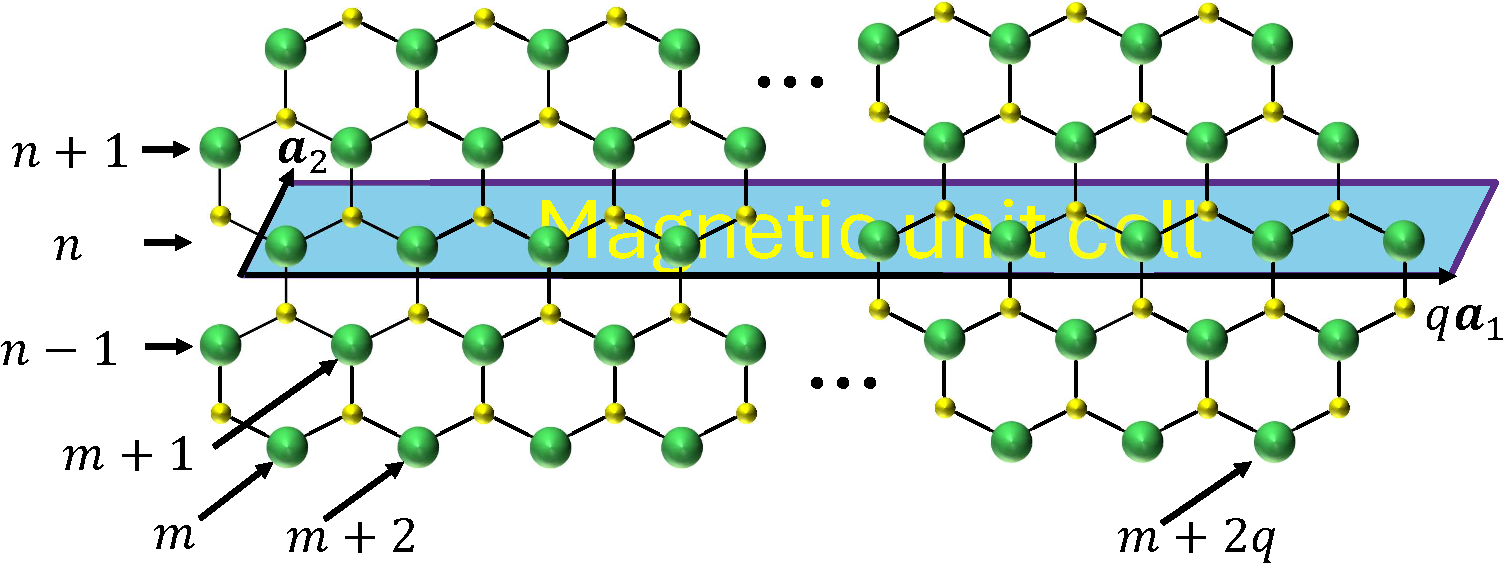
\includegraphics[width=\linewidth]{pic/magneticUC_cut.pdf}
	\caption[Magnetic unit cell for TMD monolayers.]{\label{fig:Mag UC}Magnetic unit cell for TMD monolayers.}
\end{figure}
%Hinh. 

In Section~3.1, we ignored the sum over of relative positions $\mathbf{r}_{i}$ in Eq.~(2.3) as the orbitals of X atoms were neglected. However, the magnetic unit cell consits $2q$ atom M. We now define a new basis set of $6q$ atomic orbitals $\{ \phi_{j}(\mathbf{r} - \mathbf{r}_{i}) \}$ where $j=1,2,3$ and $\mathbf{r}_{i} \in \text{MUC}$.
%Here, $\mathbf{r}_{i} = (x_{i},y_{i}) = \frac{ma}{2}\hat{x} + \frac{na\sqrt{3}}{2}\hat{y}$. 
The new basis function now is
\begin{gather}
	\psi_{\lambda,\mathbf{k}}(\mathbf{r}) = \sum_{j}^{3}\sum_{i}^{2q} C_{ji}^{\lambda}(\mathbf{k}) \sum_{{\alpha}} e^{i\mathbf{k}\cdot(\mathbf{R}_{\alpha} + \mathbf{r}_{i})} \phi_{j}(\mathbf{r} - \mathbf{R}_{\alpha} - \mathbf{r}_{i}).
\end{gather}
Here, we set $\mathbf{r}_{i}$ refers to the position of an atom in a unit cell, while $\mathbf{R}_{\alpha}$ denotes the position of different unit cells.
The Hamiltonian matrix elements in the new basis is written as
\begin{equation}
	\begin{aligned}
		H_{jj'}^{ii'}(\mathbf{k})
		&= \sum_{{\alpha}}\sum_{{\beta}} e^{i \mathbf{k} \cdot (\mathbf{R}_{\beta} - \mathbf{R}_{\alpha} + \mathbf{r}_{i'} - \mathbf{r}_{i})}  \bra{\phi_{j}(\mathbf{r} - \mathbf{R}_{\alpha} - \mathbf{r}_{i})} \left[-\tfrac{\hbar^{2} \boldsymbol{\nabla}^{2}}{2m} + U_{0}\right] \ket{\phi_{j}(\mathbf{r} - \mathbf{R}_{\beta} - \mathbf{r}_{i'})} \\
		&=\sum_{{\alpha}}\sum_{{\beta}} e^{i \mathbf{k} \cdot (\mathbf{R}_{\beta} - \mathbf{R}_{\alpha} + \mathbf{r}_{m',n'} - \mathbf{r}_{m,n})}  \bra{\phi_{j}(\mathbf{r} - \mathbf{R}_{\alpha} - \mathbf{r}_{m,n})} \left[-\tfrac{\hbar^{2} \boldsymbol{\nabla}^{2}}{2m} + U_{0}\right] \ket{\phi_{j}(\mathbf{r} - \mathbf{R}_{\beta} - \mathbf{r}_{m',n'})} .
	\end{aligned}
\end{equation}
Now we center our system at $\mathbf{r}'=\mathbf{r} - \mathbf{R}_{\alpha} - \mathbf{r}_{m,n}$ and define $\mathbf{R}_{\gamma} = \mathbf{R}_{\alpha} - \mathbf{R}_{\beta}$. We get
\begin{gather}
	H_{jj'}^{ii'}(\mathbf{k})
	= \sum_{{\alpha}}\sum_{{\gamma}} e^{-i \mathbf{k} \cdot (\mathbf{R}_{\gamma} + \mathbf{r}_{m,n} - \mathbf{r}_{m',n'})}  \bra{\phi_{j}(\mathbf{r})} \left[-\tfrac{\hbar^{2} \boldsymbol{\nabla}^{2}}{2m} + U_{0}\right] \ket{\phi_{j}(\mathbf{r} + \mathbf{R}_{\gamma} + \mathbf{r}_{m,n} - \mathbf{r}_{m',n'})}.
\end{gather}
Taking the sum over $\mathbf{R}_{\gamma}$ considering only \ac{NN}, \ac{NNN}, \ac{TNN} such that $\abs{\mathbf{R}_{\gamma}} \leq a$. The lattice vectors that satisfying this condition is $\mathbf{R}_{\gamma} = 0$. 
%We can choose $\mathbf{R}_{\alpha} = \mathbf{0}$, this will not affect the Hamiltonian. In fact, the sum over $\mathbf{R}$ is only considering the \ac{NN}, \ac{NNN}, \ac{TNN} atoms, and replacing $\mathbf{R}$ is equivalent to redefining dummy variables in the equation.
%and replacing $\mathbf{r}_{i} = \left(m \frac{a}{2}, n \frac{a\sqrt{3}}{2}\right)$, $\mathbf{r}_{i'} = \left(m' \frac{a}{2}, n' \frac{a\sqrt{3}}{2}\right)$, notice that $i = (m,n)$ 
Since only the \ac{NN}, \ac{NNN} and \ac{TNN} are considered, the matrix elements $\bra{\phi_{j}(\mathbf{r})} \left[-\tfrac{\hbar^{2} \boldsymbol{\nabla}^{2}}{2m} + U_{0}\right] \ket{\phi_{j}(\mathbf{r} + \mathbf{r}_{m,n} - \mathbf{r}_{m',n'})}$ are nonzero when $\mathbf{r}_{m',n'} = \mathbf{r}_{m,n} + \mathbf{R}$, where $\mathbf{R} = 0$ or a displacement vector connecting to a \ac{NN}, \ac{NNN}, \ac{TNN} atoms, the Hamiltonian matrix elemtents are written in the form

\begin{gather}
	H_{jj'}^{ii'}(\mathbf{k}) =\sum_{\mathbf{R}} e^{i \mathbf{k}\cdot \mathbf{R}} \bra{\phi_{j}(\mathbf{r})} \left[-\f{\hbar^{2} \boldsymbol{\nabla}^{2}}{2m} + U_{0}(\mathbf{r})\right] \ket{\phi_{j'}(\mathbf{r}-\mathbf{R})}\delta_{m + \Delta m_{\mathbf{R}},m'} \delta_{n + \Delta n_{\mathbf{R}},n'},
\end{gather}
here ($\Delta m_{\mathbf{R}}, \Delta n_{\mathbf{R}}$) the hopping relative coordinates are given in \hyperref[Table 2.1]{Table 3.1}. 
%, we define our hopping terms in the new basis is given by
%\begin{gather}
%	H_{jj'}^{ii'}(\mathbf{k}) = \sum_{{\alpha}}\sum_{{\gamma}} e^{-i \mathbf{k}\cdot \mathbf{R}_{\gamma}} \bra{\phi_{j}(\mathbf{r})} \left[-\f{\hbar^{2} \boldsymbol{\nabla}^{2}}{2m} + U_{0}(\mathbf{r})\right] \ket{\phi_{j'}(\mathbf{r}+\mathbf{R}_{\gamma})}\delta_{i,i'}.
%\end{gather}

One can regconize that Eq.~(3.32) resembles Eq.~(3.4). Additionally, the equation not only describes the hopping between magnetic unit cells but also accounts for hopping between sites within magnetic unit cells. To address the previous question, it is important to note that we have enlarged the original unit cell into a magnetic unit cell, which now contains $2q$ atoms M. The neighbor interactions are preserved inside the ``supercell'', but they now involve neighboring magnetic unit cells due to the enlarged cell structure. The Hamiltonian has a discrete tranlastional invariance with a unit cell carrying $2q$ unit cells along the $x$ axis.

%The last step is to develop the matrix Hamiltonian elements. This can be obtained by taking the sum over $\mathbf{R}$ in Eq. (2.31). We can choose $\mathbf{R}_{\alpha} = \mathbf{0}$, this will not affect the Hamiltonian. In fact, the sum over $\mathbf{R}$ is only considering the \ac{NN}, \ac{NNN}, \ac{TNN} atoms, and replacing $\mathbf{R}$ is equivalent to redefining dummy variables in the equation, 
The Hamiltonian with the Peierls phase now is
\begin{gather}
	H_{jj'}^{ii'}(\mathbf{k}) =\sum_{\mathbf{R}} e^{i \theta_{m,n}^{m + \Delta m_{\mathbf{R}},n + \Delta n_{\mathbf{R}}} } e^{i \mathbf{k}\cdot \mathbf{R}} \bra{\phi_{j}(\mathbf{r})} \left[-\tfrac{\hbar^{2} \boldsymbol{\nabla}^{2}}{2m} + U_{0}(\mathbf{r})\right] \ket{\phi_{j'}(\mathbf{r}-\mathbf{R})}\delta_{m + \Delta m_{\mathbf{R}},m'} \delta_{n + \Delta n_{\mathbf{R}},n'}.
\end{gather}
%\begin{equation}
%	\begin{aligned}
	%		& H_{jmnj'm'n'}(\mathbf{k})
	%		= e^{i\theta_{m,n}^{m,n}}e^{i\mathbf{k} \cdot (\mathbf{0} - \mathbf{0})} \bra{\phi_{j}(\mathbf{r})} H_{0} \ket{\phi_{j'}(\mathbf{r})}\delta_{m,m'}^{n,n'}                             
	%		 + e^{i\theta_{m,n}^{m+2,n}}e^{i\mathbf{k} \cdot (\mathbf{R}_{1} - \mathbf{0})} \bra{\phi_{j}(\mathbf{r})} H_{0} \ket{\phi_{j'}(\mathbf{r}-\mathbf{R}_{1})}\delta_{m+2,m}^{n,n'}     \\
	%		& + e^{i\theta_{m,n}^{m-2,n}}e^{i\mathbf{k} \cdot (\mathbf{R}_{4} - \mathbf{0})} \bra{\phi_{j}(\mathbf{r})} H_{0} \ket{\phi_{j'}(\mathbf{r}-\mathbf{R}_{4})}\delta_{m-2,m'}^{n,n'}    \\
	%		& + e^{i\theta_{m,n}^{m+1,n-1}}e^{i\mathbf{k} \cdot (\mathbf{R}_{2} - \mathbf{0})} \bra{\phi_{j}(\mathbf{r})} H_{0} \ket{\phi_{j'}(\mathbf{r}-\mathbf{R}_{2})}\delta_{m+1,m}^{n-1,n'} \\
	%		& + e^{i\theta_{m,n}^{m-1,n-1}}e^{i\mathbf{k} \cdot (\mathbf{R}_{3}-\mathbf{0})} \bra{\phi_{j}(\mathbf{r})} H_{0} \ket{\phi_{j'}(\mathbf{r}-\mathbf{R}_{3})}\delta_{m-1,m'}^{n-1,n'}  \\
	%		& + e^{i\theta_{m,n}^{m-1,n+1}}e^{i\mathbf{k} \cdot (\mathbf{R}_{5}-\mathbf{0})} \bra{\phi_{j}(\mathbf{r})} H_{0} \ket{\phi_{j'}(\mathbf{r}-\mathbf{R}_{5})}\delta_{m-1,m'}^{n+1,n'}  \\
	%		& + e^{i\theta_{m,n}^{m+1,n+1}}e^{i\mathbf{k} \cdot (\mathbf{R}_{6}-\mathbf{0})} \bra{\phi_{j}(\mathbf{r})} H_{0} \ket{\phi_{j'}(\mathbf{r}-\mathbf{R}_{6})}\delta_{m+1,m'}^{n+1,n'} \\
	%		& + e^{i\theta_{m,n}^{m+3,n-1}}e^{i\mathbf{k} \cdot (\tilde{\mathbf{R}}_{1}-\mathbf{0})} \bra{\phi_{j}(\mathbf{r})} H_{0} \ket{\phi_{j'}(\mathbf{r}-\tilde{\mathbf{R}}_{1})}\delta_{m+3,m'}^{n-1,n'} \\
	%		& + e^{i\theta_{m,n}^{m,n-2}}e^{i\mathbf{k} \cdot (\tilde{\mathbf{R}}_{2}-\mathbf{0})} \bra{\phi_{j}(\mathbf{r})} H_{0} \ket{\phi_{j'}(\mathbf{r}-\tilde{\mathbf{R}}_{2})}\delta_{m,m'}^{n-2,n'} \\
	%		& + e^{i\theta_{m,n}^{m-3,n-1}}e^{i\mathbf{k} \cdot (\tilde{\mathbf{R}}_{3}-\mathbf{0})} \bra{\phi_{j}(\mathbf{r})} H_{0} \ket{\phi_{j'}(\mathbf{r}-\tilde{\mathbf{R}}_{3})}\delta_{m-3,m'}^{n-1,n'} \\
	%		& + e^{i\theta_{m,n}^{m-3,n+1}}e^{i\mathbf{k} \cdot (\tilde{\mathbf{R}}_{4}-\mathbf{0})} \bra{\phi_{j}(\mathbf{r})} H_{0} \ket{\phi_{j'}(\mathbf{r}-\tilde{\mathbf{R}}_{4})}\delta_{m-3,m'}^{n+1,n'} \\
	%		& + e^{i\theta_{m,n}^{m,n+2}}e^{i\mathbf{k} \cdot (\tilde{\mathbf{R}}_{5}-\mathbf{0})} \bra{\phi_{j}(\mathbf{r})} H_{0} \ket{\phi_{j'}(\mathbf{r}-\tilde{\mathbf{R}}_{5})}\delta_{m,m'}^{n+2,n'} \\
	%		& + e^{i\theta_{m,n}^{m+3,n+1}}e^{i\mathbf{k} \cdot (\tilde{\mathbf{R}}_{6}-\mathbf{0})} \bra{\phi_{j}(\mathbf{r})} H_{0} \ket{\phi_{j'}(\mathbf{r}-\tilde{\mathbf{R}}_{6})}\delta_{m+3,m'}^{n+1,n'} \\
	%		& + e^{i\theta_{m,n}^{m+4,n}}e^{i\mathbf{k} \cdot (\mathbf{R}'_{1} - \mathbf{0})} \bra{\phi_{j}(\mathbf{r})} H_{0} \ket{\phi_{j'}(\mathbf{r}-\mathbf{R}'_{1})}\delta_{m+2,m}^{n,n'}     \\
	%		& + e^{i\theta_{m,n}^{m-4,n}}e^{i\mathbf{k} \cdot (\mathbf{R}'_{4} - \mathbf{0})} \bra{\phi_{j}(\mathbf{r})} H_{0} \ket{\phi_{j'}(\mathbf{r}-\mathbf{R}'_{4})}\delta_{m-2,m'}^{n,n'}    \\
	%		& + e^{i\theta_{m,n}^{m+2,n-2}}e^{i\mathbf{k} \cdot (\mathbf{R}'_{2} - \mathbf{0})} \bra{\phi_{j}(\mathbf{r})} H_{0} \ket{\phi_{j'}(\mathbf{r}-\mathbf{R}'_{2})}\delta_{m+1,m}^{n-1,n'} \\
	%		& + e^{i\theta_{m,n}^{m-2,n-2}}e^{i\mathbf{k} \cdot (\mathbf{R}'_{3}-\mathbf{0})} \bra{\phi_{j}(\mathbf{r})} H_{0} \ket{\phi_{j'}(\mathbf{r}-\mathbf{R}'_{3})}\delta_{m-1,m'}^{n-1,n'}  \\
	%		& + e^{i\theta_{m,n}^{m-2,n+2}}e^{i\mathbf{k} \cdot (\mathbf{R}'_{5}-\mathbf{0})} \bra{\phi_{j}(\mathbf{r})} H_{0} \ket{\phi_{j'}(\mathbf{r}-\mathbf{R}'_{5})}\delta_{m-1,m'}^{n+1,n'}  \\
	%		& + e^{i\theta_{m,n}^{m+2,n+2}}e^{i\mathbf{k} \cdot (\mathbf{R}'_{6}-\mathbf{0})} \bra{\phi_{j}(\mathbf{r})} H_{0} \ket{\phi_{j'}(\mathbf{r}-\mathbf{R}'_{6})}\delta_{m+1,m'}^{n+1,n'}, \\
	%	\end{aligned}
%\end{equation}
Simplizing Eq.~(3.33), we get the Hamiltonian for the magnetic unit cell
%\begin{equation}
%	\begin{aligned}
	%		& H_{ii'}^{jj'}(\mathbf{k})
	%		= \bra{\phi_{j}(\mathbf{r},m,n)} \left[-\tfrac{\hbar^{2}\nabla^{2}}{2m} + U_{0}\right] \ket{\phi_{j}(\mathbf{r},\mathbf{0},m,n)} \delta_{m,m}\delta_{n,n}                                                                                            \\
	%		+ & e^{-2i\alpha} e^{i\theta_{m,n}^{m+2,n}} \bra{\phi_{j}(\mathbf{r},m,n)} \left[-\tfrac{\hbar^{2}\nabla^{2}}{2m} + U_{0}\right] \ket{\phi_{j}(\mathbf{r},\mathbf{R}_{1},m,n)}\delta_{m+2,m}\delta_{n,n}                              \\
	%		+ & e^{2i\alpha} e^{i\theta_{m,n}^{m-2,n}} \bra{\phi_{j}(\mathbf{r},m,n)} \left[-\tfrac{\hbar^{2}\nabla^{2}}{2m} + U_{0}\right] \ket{\phi_{j}(\mathbf{r},\mathbf{R}_{4},m-2,n)}  \delta_{m-2,m}\delta_{n,n}                          \\
	%		+ & e^{i(\alpha - \beta)} e^{i\theta_{m,n}^{m+1,n-1}} \bra{\phi_{j}(\mathbf{r},m,n)} \left[-\tfrac{\hbar^{2}\nabla^{2}}{2m} + U_{0}\right] \ket{\phi_{j}(\mathbf{r},\mathbf{R}_{2},m+1,n-1)}                       \\
	%		+ & e^{i(-\alpha - \beta)} e^{i\theta_{m,n}^{m-1,n-1}} \bra{\phi_{j}(\mathbf{r},m,n)} \left[-\tfrac{\hbar^{2}\nabla^{2}}{2m} + U_{0}\right] \ket{\phi_{j}(\mathbf{r},\mathbf{R}_{3},m-1,n-1)}     \\
	%		+ & e^{i(-\alpha + \beta)} e^{i\theta_{m,n}^{m-1,n+1}} \bra{\phi_{j}(\mathbf{r},m,n)} \left[-\tfrac{\hbar^{2}\nabla^{2}}{2m} + U_{0}\right] \ket{\phi_{j}(\mathbf{r},\mathbf{R}_{5},m-1,n+1)}                       \\
	%		+ & e^{i(\alpha + \beta)} e^{i\theta_{m,n}^{m+1,n+1}} \bra{\phi_{j}(\mathbf{r},m,n)} \left[-\tfrac{\hbar^{2}\nabla^{2}}{2m} + U_{0}\right] \ket{\phi_{j}(\mathbf{r},\mathbf{R}_{6},m+1,n+1)}  . \\
	%	\end{aligned}
%\end{equation}
%\begin{equation}
%	\begin{aligned}
	%		& H_{ii'}^{jj'}(\mathbf{k})
	%		= \bra{\phi_{j}(\mathbf{r} -  m \mathbf{a}_{1} - n\mathbf{a}_{2})} \left[-\frac{\hbar^{2}\nabla^{2}}{2m} + U_{0}\right] \ket{\phi_{j}(\mathbf{r} -  m \mathbf{a}_{1} - n\mathbf{a}_{2})} \delta_{m,m'}^{n,n'}                                                                                                \\
	%		+ & e^{i\mathbf{k}\cdot\mathbf{a}_{1}} e^{i\theta_{m,n}^{m',n'}} \bra{\phi_{j}(\mathbf{r} - m \mathbf{a}_{1} - n\mathbf{a}_{2})} \left[-\frac{\hbar^{2}\nabla^{2}}{2m} + U_{0}\right] \ket{\phi_{j}(\mathbf{r} - (m+2) \mathbf{a}_{1} - n\mathbf{a}_{2})} \delta_{m+2,m'}^{n,n'}                             \\
	%		+ & e^{-i\mathbf{k}\cdot\mathbf{a}_{1}} e^{i\theta_{m,n}^{m',n'}} \bra{\phi_{j}(\mathbf{r} - m \mathbf{a}_{1} - n\mathbf{a}_{2})} \left[-\frac{\hbar^{2}\nabla^{2}}{2m} + U_{0}\right] \ket{\phi_{j}(\mathbf{r} - (m-2) \mathbf{a}_{1} - n'\mathbf{a}_{2})} \delta_{m-2,m'}^{n,n'}                           \\
	%		+ & e^{i\mathbf{k}\cdot\mathbf{a}_{2}} e^{i\theta_{m,n}^{m',n'}} \bra{\phi_{j}(\mathbf{r} - m \mathbf{a}_{1} - n\mathbf{a}_{2})} \left[-\frac{\hbar^{2}\nabla^{2}}{2m} + U_{0}\right] \ket{\phi_{j}(\mathbf{r} - (m+1) \mathbf{a}_{1} - (n+1)\mathbf{a}_{2})} \delta_{m',m+1}^{n',n+1}                       \\
	%		+ & e^{i\mathbf{k}\cdot(\mathbf{a}_{2} - \mathbf{a}_{1})} e^{i\theta_{m,n}^{m',n'}} \bra{\phi_{j}(\mathbf{r} - m \mathbf{a}_{1} - n\mathbf{a}_{2})} \left[-\frac{\hbar^{2}\nabla^{2}}{2m} + U_{0}\right] \ket{\phi_{j}(\mathbf{r} - (m-1) \mathbf{a}_{1} - (n+1)\mathbf{a}_{2})} \delta_{m',m-1}^{n',n+1}    \\
	%		+ & e^{-i\mathbf{k}\cdot\mathbf{a}_{2}} e^{i\theta_{m,n}^{m',n'}} \bra{\phi_{j}(\mathbf{r} - m \mathbf{a}_{1} - n\mathbf{a}_{2})} \left[-\frac{\hbar^{2}\nabla^{2}}{2m} + U_{0}\right] \ket{\phi_{j}(\mathbf{r} - (m-1) \mathbf{a}_{1} - (n-1)\mathbf{a}_{2})} \delta_{m',m-1}^{n',n-1}                      \\
	%		+ & e^{i\mathbf{k}\cdot(-\mathbf{a}_{2} + \mathbf{a}_{1})} e^{i\theta_{m,n}^{m',n'}} \bra{\phi_{j}(\mathbf{r} - m \mathbf{a}_{1} - n\mathbf{a}_{2})} \left[-\frac{\hbar^{2}\nabla^{2}}{2m} + U_{0}\right] \ket{\phi_{j}(\mathbf{r} - (m+1) \mathbf{a}_{1} - (n-1)\mathbf{a}_{2})} \delta_{m',m+1}^{n',n-1} . \\
	%	\end{aligned}
%\end{equation}

%Note that $\mathbf{a}_{1} = \mathbf{R}_{1}$, $\mathbf{a}_{2} = \mathbf{R}_{6}$, $-\mathbf{a}_{2} = \mathbf{R}_{3}$, $\mathbf{a}_{2} - \mathbf{a}_{1} = \mathbf{R}_{5}$ and $-\mathbf{a}_{2}+\mathbf{a}_{1} = \mathbf{R}_{2}$.

% Note that
%\begin{gather}
%	\begin{cases}
	%		e^{i k_{x} a} \phi_{j} \left(m \frac{a}{2},y\right) = \phi_{j} \left((m+2)\frac{a}{2},y\right),  \\
	%		e^{-i k_{x} a} \phi_{j} \left(m\frac{a}{2},y\right) = \phi_{j} \left((m-2)\frac{a}{2},y\right) , \\
	%		e^{\pm i k_{x} \frac{a}{2}} e^{\pm i k_{y} \frac{a\sqrt{3}}{2}} \phi_{j} \left(m \frac{a}{2},n \frac{a\sqrt{3}}{2}\right) = e^{\pm i k_{y} \frac{a\sqrt{3}}{2}}\phi_{j} \left((m \pm 1)\frac{a}{2},n\frac{a\sqrt{3}}{2}\right).
	%	\end{cases}
%\end{gather}
%Consequently the Hamiltonian matrix in the new basis is written as
%\begin{equation}
%	\begin{aligned}
	%		H_{jj'}(\mathbf{k})
	%		 & = E_{jj'}(\mathbf{0}) \delta_{m,m} + e^{i\theta_{m,n}^{m',n'}} E_{jj'}(\mathbf{R}_{1}) \delta_{m,m+2} + e^{i\theta_{m,n}^{m',n'}} e^{- i k_{y} \frac{a\sqrt{3}}{2}} E_{jj'}(\mathbf{R}_{2}) \delta_{m,m+1}    \\
	%		 & + e^{i\theta_{m,n}^{m',n'}} e^{- i k_{y} \frac{a\sqrt{3}}{2}} E_{jj'}(\mathbf{R}_{3}) \delta_{m,m - 1} + e^{i\theta_{m,n}^{m',n'}} E_{jj'}(\mathbf{R}_{4}) \delta_{m,m + 2}                                  \\
	%		 & + e^{i\theta_{m,n}^{m',n'}} e^{i k_{y} \frac{a\sqrt{3}}{2}} E_{jj'}(\mathbf{R}_{5}) \delta_{m,m - 1} + e^{i\theta_{m,n}^{m',n'}} e^{ i k_{y} \frac{a\sqrt{3}}{2}} E_{jj'}(\mathbf{R}_{6}) \delta_{m,m + 1} .
	%	\end{aligned}
%\end{equation}

%By substituting Eq (2.32) into Eq (2.35), consequently the Hamiltonian matrix in the new basis is written as
\begin{equation}
	\begin{aligned}
		&H_{jmnj'm'n'}(\mathbf{k})
		= \mathcal{E}_{jj'}(\mathbf{0}) \delta_{m,m'} \delta_{n,n'} + e^{i\mathbf{k} \cdot \mathbf{R}_{1}}\mathcal{E}_{jj'}(\mathbf{R}_{1}) \delta_{m+2,m'}\delta_{n,n'} + e^{i\mathbf{k} \cdot \mathbf{R}_{4}}\mathcal{E}_{jj'}(\mathbf{R}_{4})  \delta_{m-2,m'} \delta_{n,n'}  \\
		& + e^{-i\pi(m + 1/2)\Phi/\Phi_{0}}e^{i\mathbf{k} \cdot \mathbf{R}_{2}} \mathcal{E}_{jj'}(\mathbf{R}_{2}) \delta_{m+1,m'}\delta_{n-1,n'} + e^{-i\pi(m - 1/2)\Phi/\Phi_{0}} e^{i\mathbf{k} \cdot \mathbf{R}_{3}} \mathcal{E}_{jj'}(\mathbf{R}_{3}) \delta_{m-1,m'}\delta_{n-1,n'} \\
		& + e^{i\pi(m - 1/2)\Phi/\Phi_{0}} e^{i\mathbf{k} \cdot \mathbf{R}_{5}} \mathcal{E}_{jj'}(\mathbf{R}_{5}) \delta_{m-1,m'}\delta_{n+1,n'} + e^{i\pi(m + 1/2)\Phi/\Phi_{0}} e^{i\mathbf{k} \cdot \mathbf{R}_{6}} \mathcal{E}_{jj'}(\mathbf{R}_{6}) \delta_{m+1,m'}\delta_{n+1,n'} \\
		& + e^{- i\pi(m + 3/2)\Phi/\Phi_{0} } e^{i \mathbf{k} \cdot \tilde{\mathbf{R}}_{1}} \mathcal{E}_{jj'}(\tilde{\mathbf{R}}_{1}) \delta_{m+3,m'}\delta_{n-1,n'} + e^{- 2i\pi m\Phi/\Phi_{0} } e^{i \mathbf{k} \cdot \tilde{\mathbf{R}}_{2}} \mathcal{E}_{jj'}(\tilde{\mathbf{R}}_{2}) \delta_{m,m'}\delta_{n-2,n'} \\
		& + e^{- i\pi(m - 3/2)\Phi/\Phi_{0} } e^{i \mathbf{k} \cdot \tilde{\mathbf{R}}_{3}} \mathcal{E}_{jj'}(\tilde{\mathbf{R}}_{3}) \delta_{m-3,m'}\delta_{n-1,n'} + e^{ i\pi (m-3/2)\Phi/\Phi_{0} } e^{i \mathbf{k} \cdot \tilde{\mathbf{R}}_{4}} \mathcal{E}_{jj'}(\tilde{\mathbf{R}}_{4}) \delta_{m-3,m'}\delta_{n+1,n'} \\
		& + e^{2 i\pi m \Phi/\Phi_{0} } e^{i \mathbf{k} \cdot \tilde{\mathbf{R}}_{5}} \mathcal{E}_{jj'}(\tilde{\mathbf{R}}_{5}) \delta_{m,m'}\delta_{n+2,n'} + e^{ i\pi (m+3/2)\Phi/\Phi_{0} } e^{i \mathbf{k} \cdot \tilde{\mathbf{R}}_{6}} \mathcal{E}_{jj'}(\tilde{\mathbf{R}}_{6})\delta_{m+3,m'}\delta_{n+1,n'} \\
		& + e^{i \mathbf{k} \cdot \mathbf{R}'_{1}} \mathcal{E}_{jj'}(\mathbf{R}'_{1}) \delta_{m+4,m'}\delta_{n,n'} + e^{-2i\pi(m + 1)\Phi / \Phi_{0}} e^{i \mathbf{k} \cdot \mathbf{R}'_{2}} \mathcal{E}_{jj'}(\mathbf{R}'_{2}) \delta_{m+2,m'}\delta_{n-2,n'}  \\
		& + e^{-2i\pi(m - 1)\Phi / \Phi_{0}} e^{i \mathbf{k} \cdot \mathbf{R}'_{3}} \mathcal{E}_{jj'}(\mathbf{R}'_{3}) \delta_{m-2,m'}\delta_{n-2,n'} + e^{i \mathbf{k} \cdot \mathbf{R}'_{4}} \mathcal{E}_{jj'}(\mathbf{R}'_{4}) \delta_{m-4,m'}\delta_{n,n'}                                 \\
		& + e^{2i\pi(m - 1)\Phi / \Phi_{0}} e^{i \mathbf{k} \cdot \mathbf{R}'_{5}} \mathcal{E}_{jj'}(\mathbf{R}'_{5}) \delta_{m-2,m'}\delta_{n+2,n'} + e^{2i\pi(m + 1)\Phi / \Phi_{0}} e^{i \mathbf{k} \cdot \mathbf{R}'_{6}} \mathcal{E}_{jj'}(\mathbf{R}'_{6}) \delta_{m+2,m'}\delta_{n+2,n'}.
	\end{aligned}
\end{equation}

%\begin{equation}
%	\begin{aligned}
	%		h_{0}
	%		 & = t_{0} \delta_{m',m}^{n',n} + e^{-i\mathbf{k} \cdot \mathbf{R}_{1}} t_{0} \delta_{m',m+2}^{n',n} + e^{-i\mathbf{k} \cdot \mathbf{R}_{4}} t_{0}  \delta_{m',m-2}^{n',n}  \\
	%		 & + e^{-2i\pi(m + 1/2)p / q}e^{-i\mathbf{k} \cdot \mathbf{R}_{2}} t_{0} \delta_{m',m+1}^{n',n-1} + e^{-2i\pi(m - 1/2)p / q} e^{-i\mathbf{k} \cdot \mathbf{R}_{3}} t_{0} \delta_{m',m-1}^{n',n-1} \\
	%		 & + e^{2i\pi(m - 1/2)p / q} e^{-i\mathbf{k} \cdot \mathbf{R}_{5}} t_{0} \delta_{m',m-1}^{n',n+1} + e^{2i\pi(m + 1/2)p / q} e^{-i\mathbf{k} \cdot \mathbf{R}_{6}} t_{0} \delta_{m',m+1}^{n',n+1}. \\
	%		 &= \epsilon_{1} \delta_{m',m}^{n',n} + e^{-2 i \alpha} t_{0} \delta_{m',m+2}^{n',n} + e^{2 i \alpha} t_{0} \delta_{m',m-2}^{n',n} + 
	%		 e^{-2i\pi(m + 1/2)p / q}e^{-i(\alpha - \beta)} t_{0} \delta_{m',m+1}^{n',n-1} \\
	%		 &+ e^{-2i\pi(m - 1/2)p / q}e^{-i(-\alpha - \beta)} t_{0} \delta_{m',m-1}^{n',n-1} + e^{2i\pi(m - 1/2)p / q}e^{-i(-\alpha + \beta)} t_{0} \delta_{m',m-1}^{n',n+1} \\
	%		 &+ e^{2i\pi(m + 1/2)p / q}e^{-i(\alpha + \beta)} t_{0} \delta_{m',m+1}^{n',n+1}
	%	\end{aligned}
%\end{equation}

Now, for given flux ratio $p/q$, only the $q$ determines the periodicity of the magnetic cell assuming $p$ and $q$ are mutually prime numbers. Eq.~(3.34) give the following matrix which must be diagonalized to obtain the energy eigenvalues
\begin{equation}
	\renewcommand{\arraystretch}{0.85}
	\begin{aligned}
		H^{\text{TB}}
		& =
		\begin{pNiceMatrix}
			V_{0}     & V_{1}      & V_{2}  \\
			V_{1}^{*} & V_{11}     & V_{12} \\
			V_{2}^{*} & V_{12}^{*} & V_{22}
		\end{pNiceMatrix},
	\end{aligned}
\end{equation}
with
\begin{equation}
	\renewcommand{\arraystretch}{0.85}
	\begin{aligned}
		H_{jj'}^{\text{TB}}
		& =
		\left(
		\begin{array}{c c c c c c c c c c c c }
			A_{jj'}^{(0)} & B_{jj'}^{(0)} & C_{jj}^{(0)} & D_{jj'}^{(0)} & E_{jj'}^{(0)} & F_{jj'}^{(0)} & 0 & \cdots & G_{jj'}^{(0)} & H_{jj'}^{(0)} & I_{jj'}^{(0)} & K_{jj'}^{(0)}\\
			K_{jj'}^{(1)} & A_{jj'}^{(1)} & B_{jj'}^{(1)} & C_{jj'}^{(1)} & D_{jj'}^{(1)} & E_{jj'}^{(1)} & F_{jj'}^{(1)} & 0 & \cdots & G_{jj'}^{(1)} & H_{jj'}^{(1)} & I_{jj'}^{(1)} \\
			I_{jj'}^{(2)} & K_{jj'}^{(2)} & A_{jj'}^{(2)} & B_{jj'}^{(2)} & C_{jj'}^{(2)} & D_{jj'}^{(2)} & E_{jj'}^{(2)} & F_{jj'}^{(2)} & 0 & \cdots & G_{jj'}^{(2)} & H_{jj'}^{(2)} \\
			%				H_{jj'}^{(2)} & I_{jj'}^{(2)} & K_{jj'}^{(2)} & A_{jj'}^{(2)} & B_{jj'}^{(2)} & C_{jj'}^{(2)} & D_{jj'}^{(2)} & E_{jj'}^{(2)} & F_{jj'}^{(2)} & 0 & \cdots& 0 & G_{jj'}^{(2)} \\
			%				G_{jj'}^{(2)} & H_{jj'}^{(2)} & I_{jj'}^{(2)} & K_{jj'}^{(2)} & A_{jj'}^{(2)} & B_{jj'}^{(2)} & C_{jj'}^{(2)} & D_{jj'}^{(2)} & E_{jj'}^{(2)} & F_{jj'}^{(2)} & 0 & \cdots& 0  \\
			\vdots & \vdots & \vdots & \vdots & \vdots & \vdots & \vdots & \vdots & \vdots & \vdots & \vdots & \vdots\\
			C_{jj'}^{(q-2)} & \cdots & \cdots & \cdots & \cdots & \cdots & \cdots & 0 & \cdots & K_{jj'}^{(q-2)} & A_{jj'}^{(q-2)} & B_{jj'}^{(q-2)} \\
			B_{jj'}^{(q-1)} & C_{jj'}^{(q-1)} & \cdots & \cdots & \cdots & \cdots & \cdots & \cdots & 0 & \cdots & K_{jj'}^{(q-1)} & A_{jj'}^{(q-1)} \\
		\end{array}
		\right),
	\end{aligned}
\end{equation}
%where $A_{jj'}^{(m)} = \mathcal{E}_{jj'}(\mathbf{R}_{2})e^{-2i\pi(m+1/2)p/q}e^{-i \mathbf{k}\cdot \mathbf{R}_{2}} + \mathcal{E}_{jj'}(\mathbf{R}_{6})e^{2i\pi(m+1/2)p/q}e^{-i \mathbf{k}\cdot \mathbf{R}_{6}}$, and $B_{jj'}^{(m)} = \mathcal{E}_{jj'}(\mathbf{R}_{3})e^{-2i\pi(m-1/2)p/q}e^{-i
	%	\mathbf{k}\cdot\mathbf{R}_{3}} + \mathcal{E}_{jj'}(\mathbf{R}_{5})e^{2i\pi(m-1/2)p/q}e^{-i\mathbf{k}\cdot \mathbf{R}_{5}}$
where $A_{jj'}^{(m)}$ is the hopping with the relative coordinates $(m,n)$, $B_{jj'}^{(m)}$ is the hopping with the relative coordinates $(m+1,n)$, and so on,
and $V_{0},V_{1},V_{2},V_{11},V_{12},V_{22}$ are submatrices of size $6q \times 6q$, see Fig.~3.4.
\begin{figure*}[htb]
	\centering
	\begin{subfigure}[b]{0.495\textwidth}
		\centering
		\includegraphics[width=0.85\linewidth]{pic/matrix_1band_TNN_q_20.pdf}
		\label{fig:3 band matrix}
	\end{subfigure}
	\begin{subfigure}[b]{0.495\textwidth}
		\centering
		\includegraphics[width=0.85\linewidth]{pic/matrix_3band_TNN_q_20.pdf}
		\label{fig:1 band matrix}
	\end{subfigure}
	\caption[A visualization of super matrix.]{
		An simple and intuitive visualization of sub-matrix $V_{0}$ for single-band(a) and matrix $H$ for three band(b) using standard plotter with $q = 10$.
	}
\end{figure*}

\chapter{\textbf{RESULTS AND DISCUSSION}}
To illustrate the applicability of the three-band \ac{TBM} developed in Chapter~3, we consider the case of monolayer MoS$_{2}$ as a representive example of \acp{TMD}. For completeness, similar calculations have been perfomed for other \ac{TMD} monolayers. The corresponding results are provided in \hyperref[appendix B]{Appendix~B}.
\section{Band structure of MoS$_{2}$ at zero magnetic field}
We begin the analysis by calculating the band structure of monolayer MoS$_2$ using the three-band tight-binding model that includes spin–orbit coupling (SOC). This model captures the essential features of the low-energy physics near the $K$ and $K'$ points of the Brillouin zone.

By solving the Hamiltonian in Eq.~(3.11), we obtain the eigenvalues of the Hamiltonian, which are evaluated across the entire Brillouin zone. These are computed over all $k$-points throughout the entire \ac{BZ}, and the corresponding band structure is illustrated in Fig.~4.1. The presence of three orbitals from the M atom in the unit cell results in three energy bands: one \ac{VB} and two \acp{CB}. When spin–orbit coupling is included, these bands split due to spin degeneracy, leading to six bands in total. Among them, the \ac{VB} exhibits a prominent spin splitting near the $K$ and $K'$ points, while the \acp{CB} remain nearly degenerate.


%The diagram in Fig. 2.8 shows the significant splitting of the valence bands at the $K$ and $K'$ points of MoS$_{2}$, caused by the \ac{SOC}, with a value of $\Delta_{\text{SOC}}^{\lambda} = 2 \lambda = 146$ meV. Although the \ac{NN} \ac{TB} model is not accurate as the TNN one, it can be seen that the \ac{NN} \ac{TB} bands agree well the \ac{TNN} results near the $K$ and $K'$ points.

This splitting is attributed to the atomic \ac{SOC} of the Mo atom, with a magnitude of $\Delta_{\text{SOC}}^{\lambda} = 2\lambda = 146$ meV. This effect is a hallmark of monolayer \acp{TMD}, playing a crucial role in spin–valley coupling and valley-selective optical properties.


\begin{figure*}[htb]
\begin{subfigure}[b]{0.495\textwidth}
	\centering
	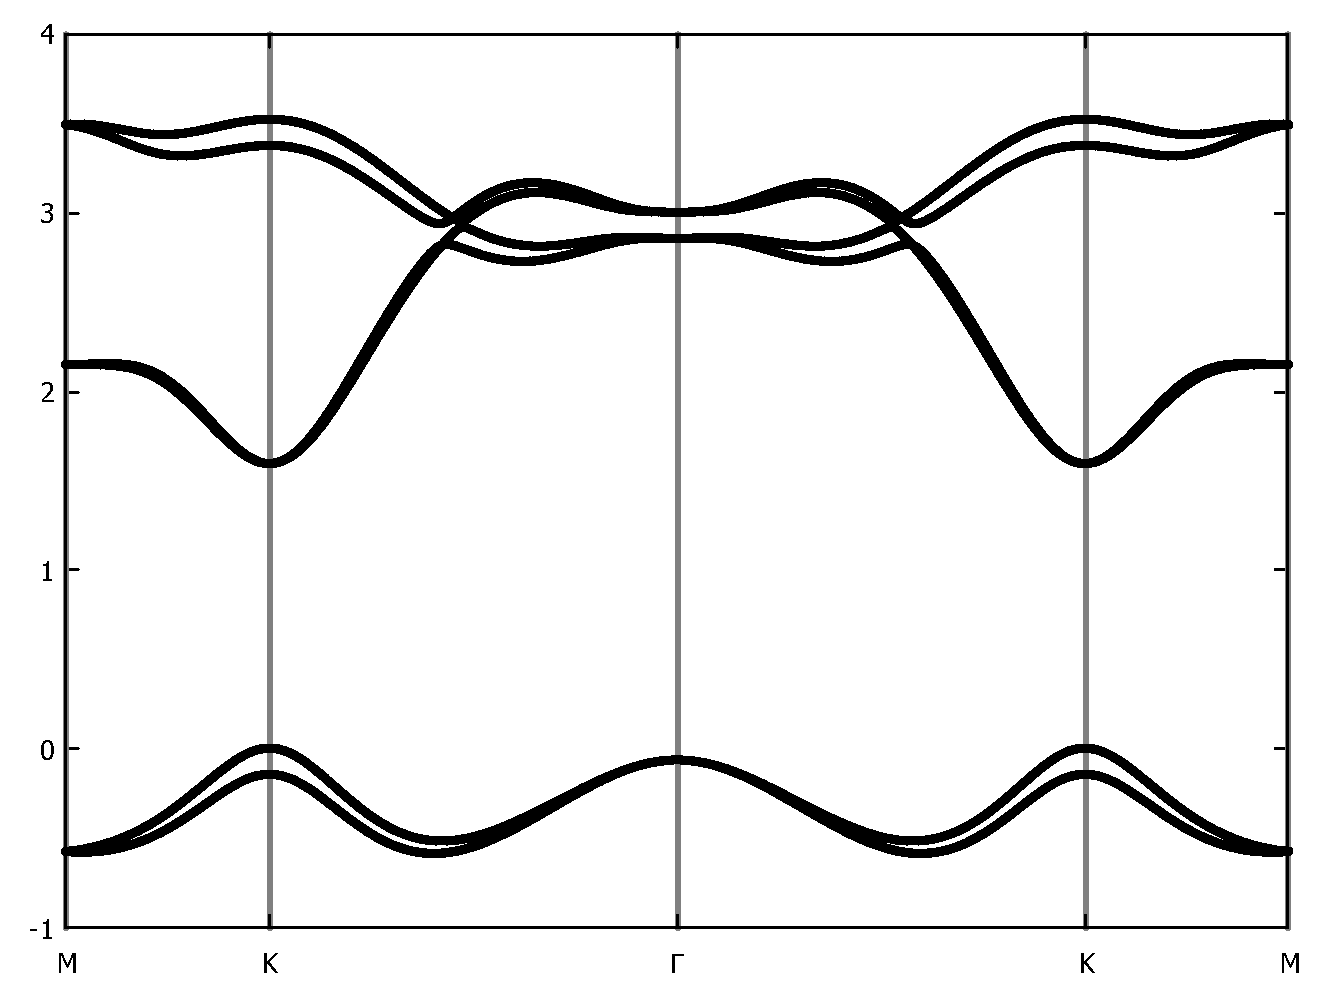
\includegraphics[width=\linewidth]{pic/bandstructureSOC.pdf}
	%\caption{\label{band structure SOC}}
\end{subfigure}
\begin{subfigure}[b]{0.495\textwidth}
	\centering
	\includegraphics[width=\linewidth]{pic/bandstructureSOCTNN.pdf}
	%\caption{\label{HB SOC}}
\end{subfigure}
\caption[Banstructure of NN and TNN monolayer MoS$_{2}$ with SOC without magnetic field.]{The band structure of monolayer MoS$_2$ in the absence of a magnetic field along the $\Gamma$–K direction exhibits significant spin splittings at the $K$ and $-K$ points, primarily due to spin–orbit coupling (SOC). Figures 4.1(a) and 4.1(b) show the results obtained using \ac{NN} and \ac{TNN} model, respectively.
}
\end{figure*}
\section{Hofstadter butterfly of monolayer MoS$_{2}$}
In this section, we explore the Hofstadter spectrum by presents the solution of Eq.~3.35. By plotting the band energies while varying the $p$, we obtain the famous Hofstadter butterfly \cite{PhysRevB.14.2239}, a complex fractal structure as seen in Fig.~4.2. This fractal spectrum is a result of two competing effects, lattice periodicity and magnectic unit cell periodicity enforced by the presence of the magnetic field. The magnetic field enters the \ac{TB} Hamiltonian only through the fraction $p/q$, which is proportional to the magnetic flux through the primitive unit cell of the lattice. In general, as the lattice geometry evolves, the area of the primitive unit cell changes $m$ times.

In this study, the Hofstadter butterfly of MoS$_2$ is generated at the $K$-point. Additionally, we compute a single-band Hofstadter butterfly (using only the conduction band) to highlight the underlying triangular lattice structure of MoS$_2$. In Fig.~4.2, for the \ac{NN} model, the Hofstadter butterfly structure clearly resembles that of a triangular lattice, as previously reported in other materials such as \cite{li2011}.


\begin{figure*}[htb]
\centering
\begin{subfigure}[b]{0.32\textwidth}
	\centering
	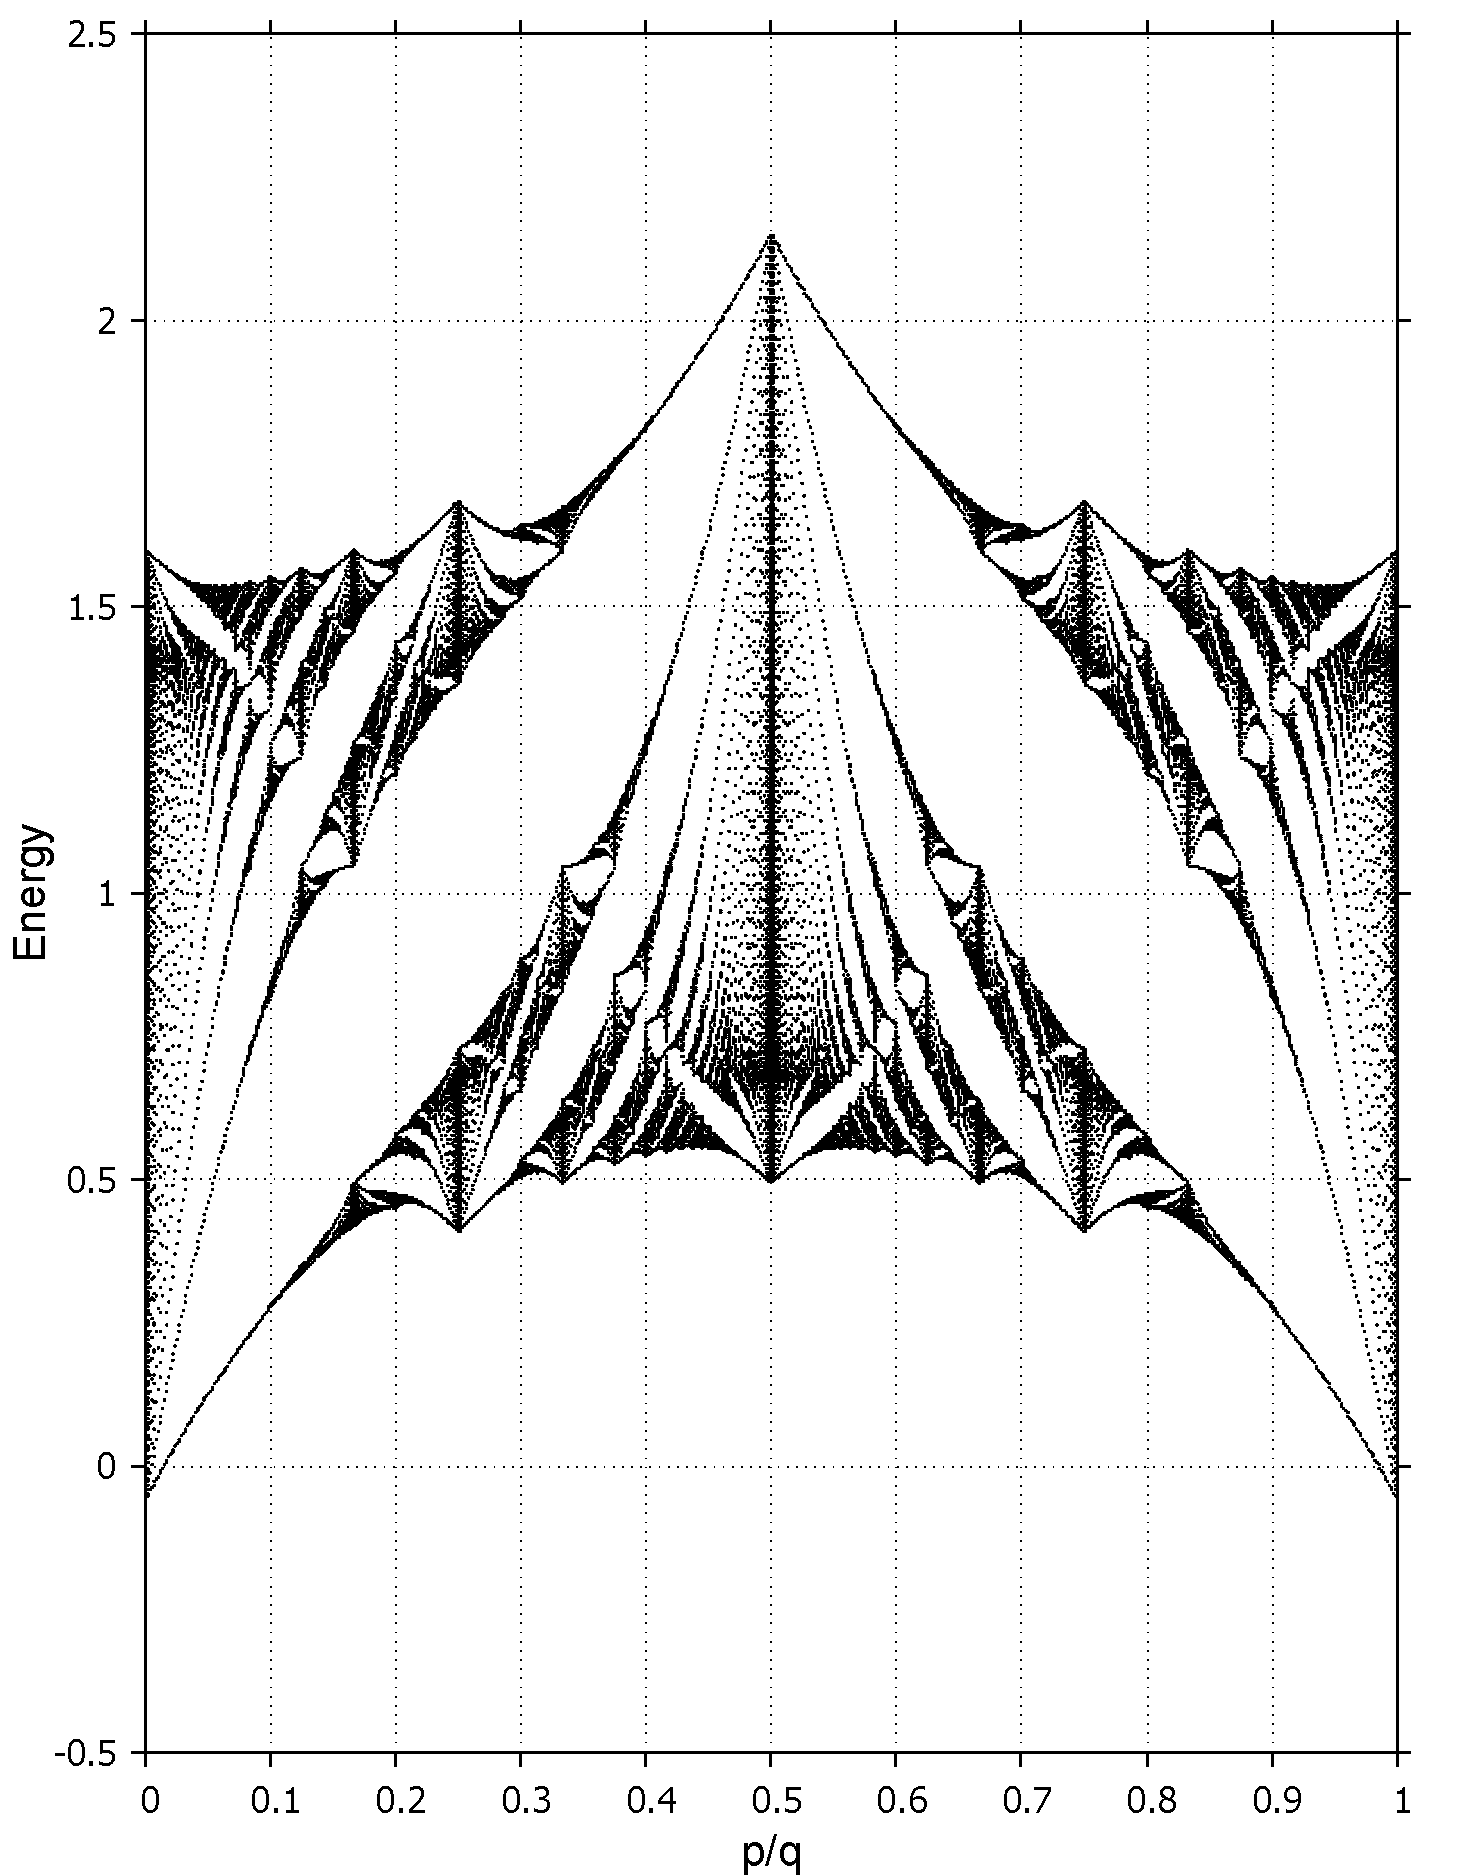
\includegraphics[width=0.95\textwidth,height=1.2\linewidth]{pic/h0_tam giac_q_797.png}
	\label{fig:3 band}
\end{subfigure}
\begin{subfigure}[b]{0.32\textwidth}
	\centering
	\includegraphics[width=0.95\textwidth,height=1.2\linewidth]{pic/h0_tam giac_TNN_LDA_q_797.png}
	\label{}
\end{subfigure}
\begin{subfigure}[b]{0.32\textwidth}
	\centering
	\includegraphics[width=0.95\textwidth,height=1.2\linewidth]{pic/h0_tam giac_TNN_GGA_q_797.png}
	\label{}
\end{subfigure}
\begin{subfigure}[b]{0.32\textwidth}
	\centering
	\includegraphics[width=0.95\textwidth,height=1.2\linewidth]{pic/3band_gnuplot_TNN_q_797.png}
	\label{fig:1 band}
\end{subfigure}
\begin{subfigure}[b]{0.32\textwidth}
	\centering
	\includegraphics[width=0.95\textwidth,height=1.2\linewidth]{pic/3band_gnuplot_TNN_LDA_q_797.png}
	\label{}
\end{subfigure}
\begin{subfigure}[b]{0.32\textwidth}
	\centering
	\includegraphics[width=0.95\textwidth,height=1.2\linewidth]{pic/3band_gnuplot_TNN_GGA_q_797.png}
	\label{}
\end{subfigure}
\caption[Hofstadter butterfly for {TMD}.]{
	Hofstadter butterfly for single-band $\ket{dz} \equiv \ket{\phi_{1}^{1}(x,y)}$(a,b,c) and all band(d,e,f) for \ac{NN} and \ac{TNN} for MoS$_2$, respectively, with $q = 797$ and vary $p$ from 1 to $q$ with field strength $B_{0} = 4.6928 \times 10^{4}$ T. Here on $x-$axis represents the flux in units of quantum flux enclosed by the unit cell and $y-$axis represents the Energy. While (b,e) use \ac{GGA} parameter, (c,f) use \ac{LDA} one.
}
\end{figure*}

Another observation is that the lattice constant $a$ and the magnetic field $B$ always appears together in an expression with the magnetic field ($\tfrac{Ba^{2}\sqrt{3}}{2}$). This quantity reflects the flux per plaquette in the super magnetic unit cell, which is relevant is the context of Aharonov-Bohm effect \cite{aharonov1959}. Since the expression involves the product $Ba^{2}$, this implies that increasing $B$ by a certain amount is mathematically equivalent to increasing $a$. In other words, for energy calculations, increasing the strength of the magnetic field is physically equivalent to increasing the lattice constant, as both affect the system in the same way through the flux per unit cell. In addition, the three-band spectrum contains a complex and rich physics insight but it seem remains the fractal structure. The main energy bands are basically \acp{LL}, which we shall discuss in the next Section. For small values of the magnetic flux ratio $p/q$, these \acp{LL} manifest sharp and well-separated energy bands. However, when increasing $p$ from 1 to $q$, each \acp{LL} go a recursive splitting into $2q$ subbands. This structure arises from the magnetic unit cell's periodicity.

The spectrum exhibits several noticeable symmetries. First, it depends only on the flux ratio $p/q$, meaning that shifting $p/q$ by an integer $c$ (i.e., $p/q \rightarrow p/q + c$) leaves the spectrum unchanged. Additionally, the spectrum remains invariant under the transformation $p/q \rightarrow -p/q$, since if $\psi$ is an eigenstate with energy $E$ for flux $p/q$, its complex conjugate $\psi^*$ is an eigenstate with the same energy for flux $-p/q$. These two symmetries are general and not specific to the MoS$_{2}$ case. However, the third symmetry involves changing $p/q$ to $p/q + 1/2$, which is equivalent to flipping the sign of the hopping energies $t_{i}$ (i.e., $t_{i} \rightarrow -t_{i}$), resulting in an inversion of the spectrum, which is concealed clearly in square lattice \cite{PhysRevB.14.2239} or honeycomb lattice \cite{rammal1985}. In contrast, for the case MoS$_{2}$, the flux going through a unit cell is already one half, making this symmetry hidden. In fact, by adding an integer $n$ to the Peierls phase, one can effectively recover this symmetry, but this modification does not correspond to any physical observable.

\begin{figure*}[htb]
	\begin{subfigure}[b]{0.495\textwidth}
		\centering
		\includegraphics[width=\linewidth]{pic/plotHofstadterButterfly_q=797_MoS2_SOC_f.png}
		%\caption{\label{band structure SOC}}
	\end{subfigure}
	\begin{subfigure}[b]{0.495\textwidth}
		\centering
		\includegraphics[width=\linewidth]{pic/plotHofstadterButterfly_q=797_MoS2_SOC_LDA.png}
		%\caption{\label{HB SOC}}
	\end{subfigure}
	\caption[Hofstadter butterfly of monolayer MoS$_{2}$ with SOC in the presence of magnetic field.]{Hofstadter butterfly of monolayer MoS$_{2}$ with SOC at $K$ point. Figures 4.3(a) and 4.3(b) show the results obtained using \ac{NN} and \ac{TNN} model, respectively. }
\end{figure*}

The role of the eight hopping constants $t$ is just to set an energy scale. Change the hopping constants amounts to stretching the butterfly spectrum vertically, which is an overall scaling to the energy levels. Thus it does not give rise to any interesting physical phenomenon.

At the very large magnetic fields, the magnetic strength overwhelms the effects of \ac{SOC}. In this work, we treat the \ac{SOC} interaction as an adjustable constant in the Hamiltonian. As a result, the \ac{SOC} induces a spin splitting in the Hofstadter spectrum, see in Fig.~4.3.

In the case of the \ac{NN} model for MoS$_{2}$, our results are consistent with those reported in Refs.~\cite{ho2014,ho2015}. However, it is worth noting that our approach is more general, as Eq.~(3.34) explicitly incorporates the variation of $\delta_{n,n'}$, which was not considered in their formulation, such as in the equations of Refs.~\cite{ho2015} or Eq.~5 of Refs.~\cite{ho2014}. In addition, we also take into account interactions with 18 neighboring atoms, a level of detail that, to the best of our knowledge, has not been included in earlier models. This extended consideration significantly increases the computational complexity and demands.



\section{Landau levels in monolayer MoS$_{2}$}
The approach in Section~2.3 is for free electrons, but near the bottom of the two-dimensional tight-binding band of \ac{TMD} we must find a regime in which the electron behaves as a nearly one(At least with a nearly free dispersion relation). 

Recalling the result obtained for the dispersion relation of an electron within the \ac{TBM}
\begin{gather}
H_{11} = 2 t_{0} (\cos 2\alpha + 2 \cos \alpha \cos \beta) + \epsilon_{1}.
\end{gather}
The dispersion energy is approximately free-electron-like by Taylor expansion to second order of $\mathbf{k}$
\begin{equation}
\begin{aligned}
	H_{11}(\mathbf{k})
	& \approx 2 t_{0} \left[1 - \frac{a^{2} k_{x}^{2}}{2} + 2\left(1 - \f{a^{2} k_{x}^{2}}{8}\right)\left(1 - \f{3a^{2} k_{y}^{2}}{8}\right)\right] \\
	& = t_{0} \f{3}{16} \left(32 + a^{4} k_{x}^{2} k_{y}^{2}\right) - t_{0} \f{3}{2} a^{2}\left(k_{x}^{2} + k_{y}^{2}\right) + \epsilon_{1} ,
\end{aligned}
\end{equation}
the term $a^{4}$ is negligibly small, then we have
\begin{equation}
\begin{aligned}
	H_{11}(\mathbf{k})
	& \approx 6 t_{0} - \f{3}{2} t_{0} a^{2} (k_{x}^{2} + k_{y}^{2}) + \epsilon_{1}.
\end{aligned}
\end{equation}
One of the ways derivation of effective mass $m^{*}$ is substitution $\hbar\mathbf{k} \rightarrow \mathbf{\Pi} + e \mathbf{A}$, with Landau gauge $\mathbf{A} = (0,Bx,0)$
\begin{equation}
\begin{aligned}
	H_{11}(\mathbf{\Pi})
	& \approx 6 t_{0} - \f{3}{2} t_{0} \f{a^{2}}{\hbar^{2}} \left[ \Pi_{x}^{2} + \left(\Pi_{y} + e B x\right)^{2}\right] + \epsilon_{1}                                                           \\
	& \approx 6 t_{0} - \f{3}{2} t_{0} \f{a^{2}}{\hbar^{2}} \Pi_{x}^{2} - \f{3}{2} t_{0} \f{a^{2}}{\hbar^{2}} (e B)^{2} \left[ x - \left(- \f{\hbar k_{y}}{eB}\right) \right]^{2} + \epsilon_{1}.
\end{aligned}
\end{equation}
The Eq (4.4) can be rewrite in the form as
\begin{gather}
E(\mathbf{\Pi}) = 6 t_{0} - \left[\f{1}{2m^{*}} \Pi_{x}^{2} + \f{1}{2} m^{*} \omega_{c}^{2}(x - x_{0})^{2}\right] + \epsilon_{1},
\end{gather}
where $m^{*} = \frac{\hbar^{2}}{3t_{0}a^{2}}$ is the effective mass and $x_{0} = \frac{\hbar k_{y}}{eB}$. Subsequently, the cyclotron frequency is
\begin{gather}
\omega_{c} = \f{eB}{m^{*}} = \f{8 \pi \sqrt{3} t_{0}}{\hbar}  \f{p}{q},
\end{gather}
and therefore the Landau levels near the bottom of the band structure can be written as
\begin{equation}
\begin{aligned}
	E_{n}
	& = 6 t_{0} - \hbar \omega_{c} (n + 1 /2) + \epsilon_{1}                    \\
	& = t_{0} \left(6 - 8\pi\sqrt{3} \f{p}{q}( n + 1 /2)\right) + \epsilon_{1},
\end{aligned}
\end{equation}
in linear order of an uniform-flux, where $n$ is Landau index. 

\begin{figure*}[htb]
\centering
\begin{subfigure}[b]{0.49\textwidth}
	\centering
	{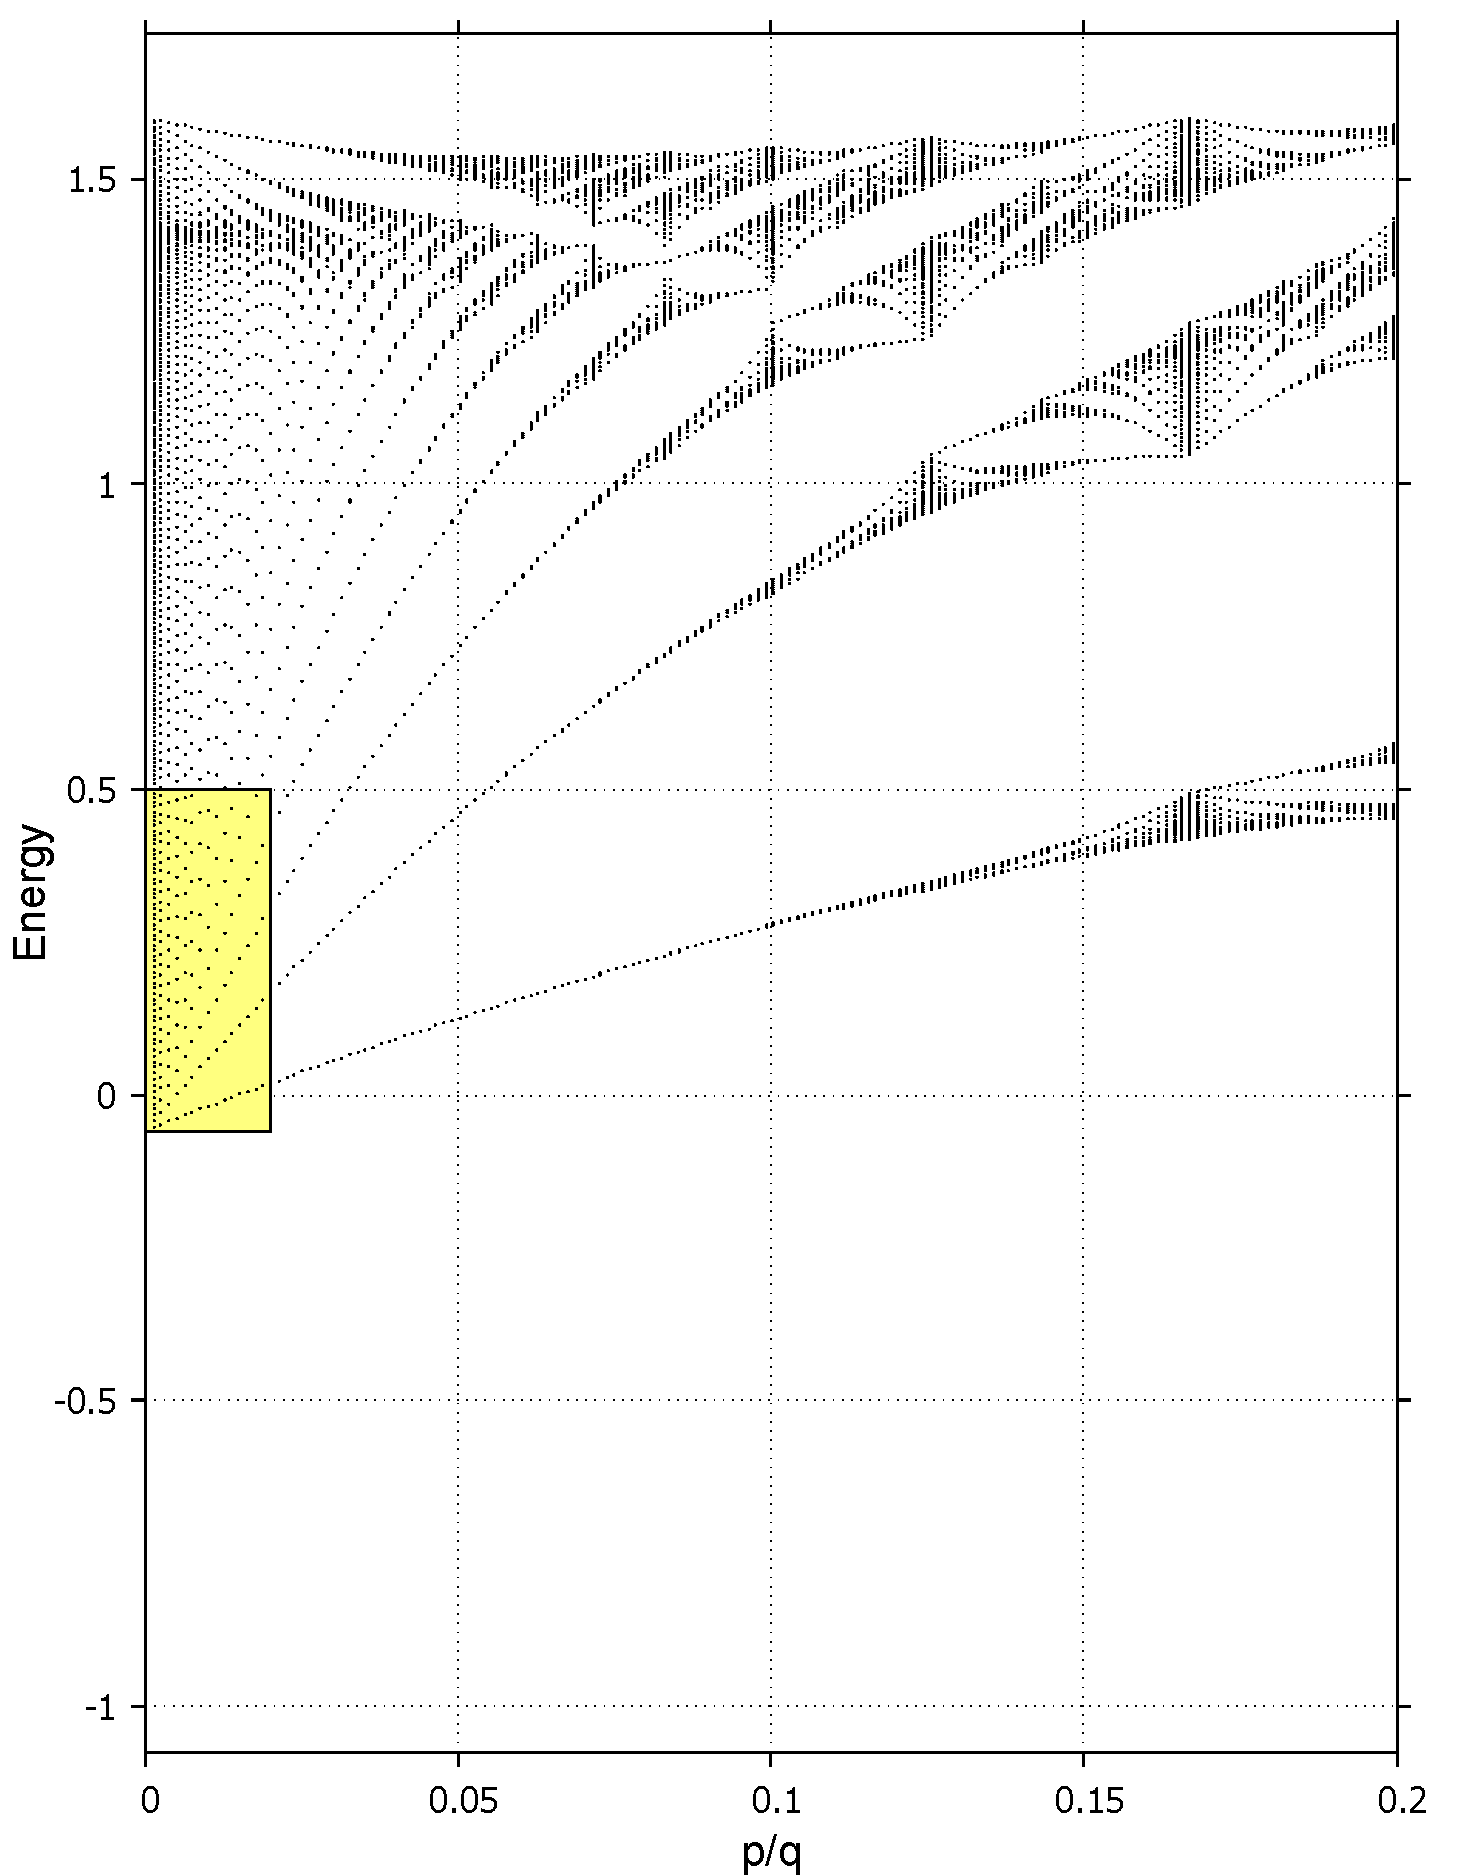
\includegraphics[width=0.85\textwidth,height=1.2\linewidth]{pic/small_area_LL.png}}
\end{subfigure}
\begin{subfigure}[b]{0.49\textwidth}
	\centering
	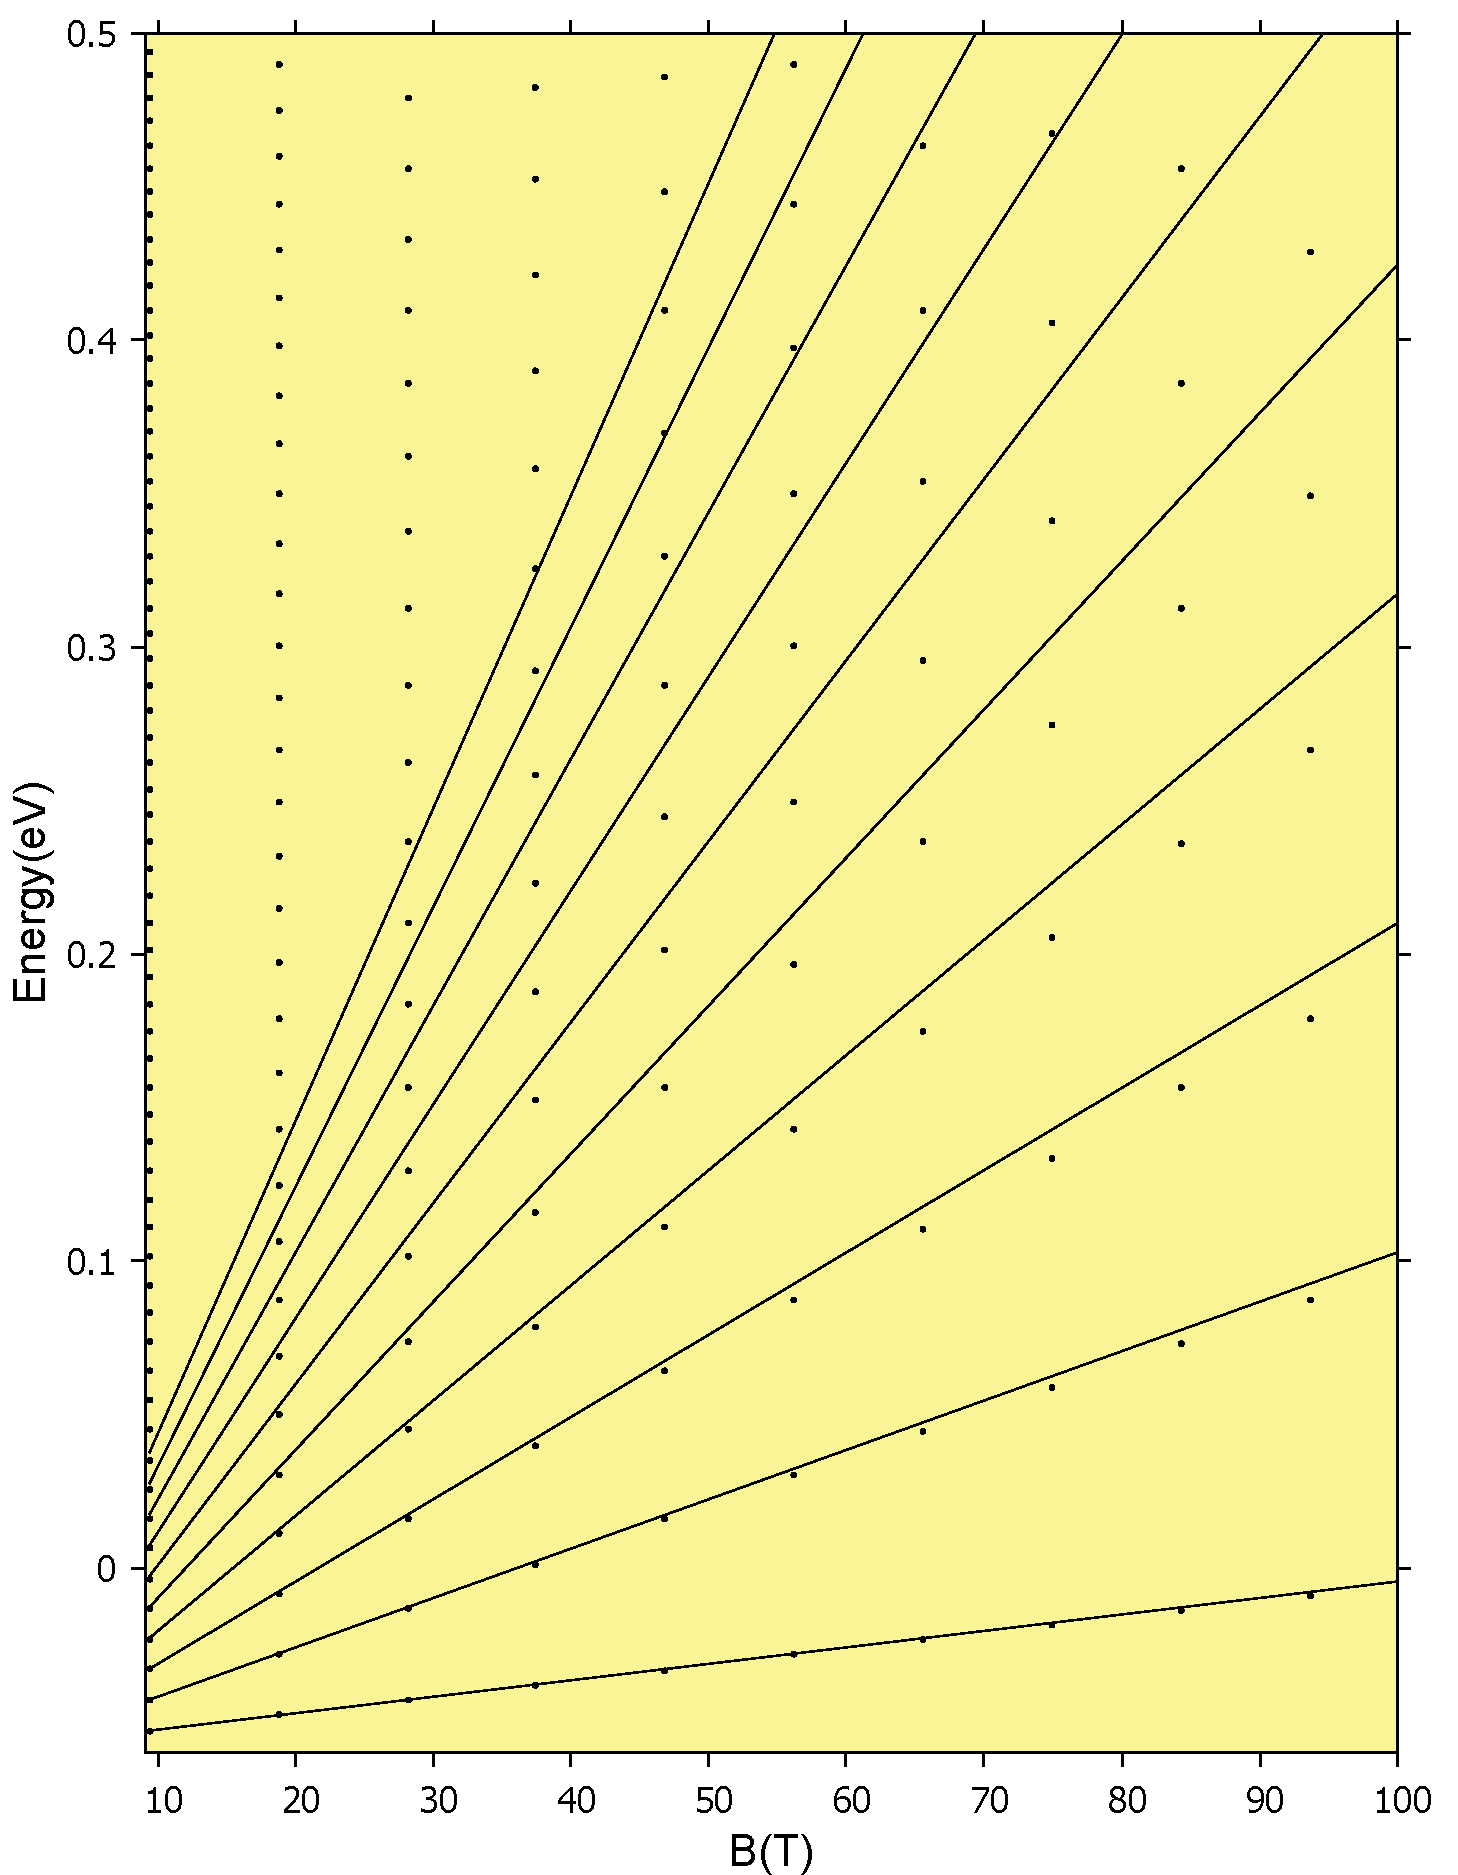
\includegraphics[width=0.85\textwidth,height=1.2\linewidth]{pic/landaulevel_h0_q_797.pdf}
\end{subfigure}
\caption[Landau levels in Hofstadter butterfly.]{
	(a) Same plot as Fig.~4.4(a) but considering a small area and (b) shows both the Landau fan diagram and the Hofstadter butterfly. Display the first $n = 30$ levels near the bottom of the conduction band for a magnetic field up to $B = 500$ T.
}
\end{figure*}

In Fig.~4.4 we compare the spectrum of a small section of single-band with $p / q = 1 / 797$, which is equivalent to small magnetic field, the spectrum of MoS$_{2}$, with the energy of Landau levels given by Eq.~(4.7) show standard equally spaced \acp{LL} \cite{Shoenberg_1984,singleton2001band,blundell2001magnetism,kittel1987quantum} near the bottom of the bands, as plotted in Fig.~4.4(b). The fan of \acp{LL} can be clearly seen emergin from the pattern in Fig.~4.4(a).

In Fig.~4.4(a), there is just single-band in case zero field, with the effective mass $m^{*} = \frac{\hbar}{3 t_{0} a^{2}}$. The numerical result for this portion of the spectrum are shown in Fig.~4.4 for $p/q \geq 1/797$. The first few \acp{LL} are clearly seen, and the asymtotic slopes $p/q$ at large $q$ given by Eq.~(4.7) are shown for comparison for the first five Landau levels at $B \leq 100$ T. At the values of $B$ the fit is not ideal, but it does seem to be improving with the decreasing $p/q$.

Figure~4.4 also displays a blowup of the low uniform magnetic field region, showing the \acp{LL} as a function of $\Phi / \Phi_{0}$. These Landau levels appear approximately linear in $B$, which is a consequence of magnetic quantization of the parabolic bands at $B = 0$~T. As the magnetic field increases, the \acp{LL} are sequentially depopulated. For example, at $B = 200$~T, the levels are completely filled up to $n = 4$, whereas at $B = 500$~T, only levels up to $n = 1$ remain filled, and higher levels are emptied. When compared with the theoretical study presented in Section~2.3, we find that the Hofstadter butterfly in the weak magnetic field regime is in excellent agreement with the predicted Landau level structure. This indicates that the model accurately captures the low-field physics.


\section{Color the Hofstadter butterfly}
In Section~2.4.2, we arrived at the Hall conductivity equation from a single subband, which is given by \cite{kohmoto1989,hatsugai1990energy,kohmoto1985topological,thouless1982}
\begin{gather}
\sigma_{xy} = \f{e^{2}}{h} \sum_{n}^{\text{occ.}} \f{1}{2\pi} \dps\oiint_{\text{{BZ}}} d k_{x} d k_{y} \Omega_{n}^{z} (\mathbf{k}).
\end{gather}
In general, the Berry curvature intergrated over a closed manifold is quantized in the units of $e^{2} / h$ and equals to the net number of monopoles inside. This number is called the Chern number and is responsible for a number of quantization effects. Therefore the Hall conductivity is quantized for a two dimensional band insulator of noninteracting electrons. By integrating the Berry curvature over the entire Brillouin zone, we arrived at the \ac{TKNN}'s formula \cite{thouless1982}
\begin{gather}
\sigma_{xy} = \f{e^{2}}{h} \nu, \quad \nu = 1,2,...
\end{gather}
$\nu$ is the Chern number.

%With the cyclotron frequency in Section 2.4, the electron energy is quantized to the Landau levels.

We, then, calculate the quantum Hall conductivity by the Streda formula \cite{streda1982}
\begin{gather}
\sigma_{xy}(B,E_{F}) = e \f{\partial N (E,B)}{\partial B} \at{E=E_{F}}{},
\end{gather}
%As show in Fig. (2.12), the Hall conductivity is quantized at colored points.
where $N(E_{F},B)$ is the number of state at fixed Fermi energy $E_{F}$. Combining Eq.~(4.9) and Eq.~(4.10), we have
\begin{gather}
	\f{\partial N}{\partial B} = \f{e}{h} \nu.	
\end{gather}
Assuming that $B$ vary slightly
\begin{gather}
	N = c + \f{e}{h}B \nu, \quad c \; \text{is constant}.
\end{gather}
Before this, we have defined $\frac{p}{q} = \frac{eBa^{2}\sqrt{3}}{2h}$, with $S = \frac{\sqrt{3} a^{2}}{2}$ is the area of the original unit cell in \hyperref[Section 3.2]{Section 3.2}. Multiply $S$ with Eq.~(4.12), we have
\begin{gather}
	N \times S = c + \f{p}{q} \nu,
\end{gather}
and the density of electron in a single band is given by $\frac{1}{Sq}$, thus when there are $r$ bands below the Fermi energy level, the density of electron for $r^{\text{th}}$ band is
\begin{gather}
	N = \f{r}{Sq}.
\end{gather}
Then, the Eq.~(4.13), is written as,
\begin{gather}
	r = c \times q + p \times \nu_{r},
\end{gather}
in this equation $r$, $q$, $p$, $\nu$ are integers, thus, $c\times q$ must be an integer. On the one hand, since $c$ is independent of $q$, then $c$ itself must be an integer, namely $s_{r}$. Thus we have
\begin{gather}
	r = q \times s_{r} + p \times \nu_{r},
\end{gather}
this equation is usually named as the Diophantine equation. While $\nu_{r}$ is the Chern number associated with the quantized Hall conductance which can be found by taking $\nu_{r}$ between $-q/2$ and $q/2$ and determining its allows conductance to be determined, $s$ is another integer that play a role in indentify the gap index.

The Hall conductivity of the lattice model for an electron in a background magnetic field can only be computed when the flux ratio $\frac{\Phi}{\Phi_{0}} = \frac{p}{q}$ is rational. In this case, we can use the TKNN formula, but with the Chern number, which used to be defined by intergrating over the Brillouin zone, now arising by intergrating over the magnetic Brillouin zone. Others derivation is in \cite{di2022linking,dana1985,avron2003}.

The Diophantine equation is crucial in understanding the quantization of Hall conductance in the Hofstadter butterfly. The Chern number $\nu$ determines the topological nature of the bands and their contribution to the Hall conductance, while the integer $s$ identifies specific energy gaps in the spectrum. These gaps are directly linked to incompressible quantum Hall states, which are of significant interest in both theoretical and experimental condensed matter physics. The solutions to the Diophantine equation are presented in Table D.1 in \hyperref[appendix D]{Appendix D}, revealing many interesting observations can be extracted from it. Firstly, we observe the occurence values of $\nu = \pm 1$ at both $r = p$ and $r = q-p$. This owing to each band being devided into $q$ subbands. Significantly, the case $r = p$, where the corresponding gap index naturally corresponds to the first gap in the Landau level. The second observation is the symmetry of the table, the value of $\nu_{r}$ is equal to $-\nu_{q-r}$. This is due, once again, to the symmetry of the butterfly.
\begin{figure*}[htb]
	\centering
	\begin{subfigure}[b]{0.495\textwidth}
		\centering
		{\includegraphics[width=\linewidth]{pic/1band_Chern_q_199_f.pdf}}
	\end{subfigure}
	\begin{subfigure}[b]{0.495\textwidth}
		\centering
		\includegraphics[width=\linewidth]{pic/3band_Chern_q_199_f.png}
	\end{subfigure}
	\caption{
		Colored points version of Hofstadter butterfly.
	}
\end{figure*}

To further explore the intricate fractal nature of the Hofstadter spectrum, we shall now achieve the colored Hofstadter butterfly. There are many ways to color the butterfly. For instance, a common approach is to color each point of the butterfly based on their Chern number, as illustrated in the Fig.~4.5. At these points, the Hall conductivity hightlights exactly quantization. However, a drawback of this method is that the butterfly may contain a dense of points, which can make it difficult to visualise fine details in the colored spectrum.

%	\begin{subfigure}[b]{0.495\textwidth}
%	\centering
%	\includegraphics[width=0.85\textwidth,height=1.2\linewidth]{pic/wannier_gnu.pdf}
%\end{subfigure}



%\begin{figure*}[htb]
%	\centering
%	\begin{subfigure}[b]{0.495\textwidth}
	%		\centering
	%		\includegraphics[width=\linewidth]{pic/1band_dataHofstadterButterfly_q_797_fix_chern.eps}
	%	\end{subfigure}
%	\begin{subfigure}[b]{0.495\textwidth}
	%		\centering
	%		\includegraphics[width=\linewidth]{pic/3band_Chern_q_797_colorplane2.png}
	%	\end{subfigure}
%	\caption[Colorplaned Hofstadter butterfly.]{
	%		q = 199 và q = 797. This color pallete was famously made by Avron\cite{avron2003}.
	%	}
%\end{figure*}
%\begin{figure*}[htb]
%	\centering
%	\begin{subfigure}[b]{0.495\textwidth}
	%		\centering
	%		\includegraphics[width=\linewidth]{pic/1band_Chern_q_797_colorplane.png}
	%	\end{subfigure}
%	\begin{subfigure}[b]{0.495\textwidth}
	%		\centering
	%		\includegraphics[width=\linewidth]{pic/3band_Chern_q_797_colorplane_f.png}
	%	\end{subfigure}
%	\caption[Colorplaned Hofstadter butterfly.]{
	%		q = 199 and q = 797. This color pallete was famously made by gnuplot.
	%	}
%\end{figure*}


Figures~4.6 and 4.7 displays the Hofstadter butterfly, color-coded according to the Hall conductance. Moreover, the number $p$ increases simultaneously with Chern number, making it challenging to maintain a fixed scale. Addressing this, we limit the Chern number scale within $-10 \leq \nu \leq 10$, any Chern number outside this range is set to zero. Regions with zero Hall conductance and the corresponding spectrum are left blank. Remarkably, the two largest gaps near the center of the figure are associated with small integers where the color coding accurately reflects their values. This idea was first made by Avron \textit{et al}\cite{avron2003}. 

\begin{figure*}[htb]
	\centering
	\begin{subfigure}[b]{0.495\textwidth}
		\centering
		{\includegraphics[width=\linewidth]{pic/1band_Chern_q_797_colorplane2.png}}
	\end{subfigure}
	\begin{subfigure}[b]{0.495\textwidth}
		\centering
		\includegraphics[width=\linewidth]{pic/3band_Chern_q_797_colorplane_f.png}
	\end{subfigure}
	\caption[Gaps color-coded Hofstadter butterfly for NN case.]{
		Gaps color-coded Hofstadter butterfly. Figures 4.6(a) and 4.6(b) show the results obtained using only \ac{NN} for single band and three band, respectively.
	}
\end{figure*}
\begin{figure*}[h]
	\centering
	\begin{subfigure}[b]{0.495\textwidth}
		\centering
		{\includegraphics[width=\linewidth]{pic/1band_Chern_q_797_TNN_colorplane.png}}
	\end{subfigure}
	\begin{subfigure}[b]{0.495\textwidth}
		\centering
		\includegraphics[width=\linewidth]{pic/3band_Chern_q_797_TNN_colorplane.png}
	\end{subfigure}
	\caption[Gaps color-coded Hofstadter butterfly for TNN case.]{
		Gaps color-coded Hofstadter butterfly for TNN case. Figures 4.7(a) and 4.7(b) show the results for single band and three band, respectively.
	}
\end{figure*}

Both figures display rich physics insights, it totally use two different methods to color the butterfly. While Fig.~4.5 assigns colors based on the sum of the Chern numbers of the occupied bands, Figs.~4.6 and 4.7 color the gap according to the Chern number that corresponded to each gap index. However, the colored spectrum do more than hightligting the topological properies of the system, they both also explain the behaviour of electrons in a symmetry lattice. Unlike the traditional Hofstadter butterfly, which highlights the energy spectrum, this version emphasizes the energy gaps by applying a color scheme to indicate different Hall conductance values. Each color represents a distinct quantized Hall conductance. Such as, doping a fixed number of electrons will causes Fermi level change, which is reflected in changes to the \ac{DOS}, caputered in Fig.~4.6. In addition as the magnetic field increases, there are fewer bands occupied. One might ask where the electrons goes. They still there, but not in the bands.


\section{Conclusions}


In our research, we have investigated the Hofstadter butterfly spectrum of monolayer MoS$_{2}$ and other transition metal dichalcogenides (TMDs) using a tight-binding three-band model. In the presence of an external magnetic field, we have explored various quantum phenomena such as Landau levels and the integer quantum Hall effect (IQHE). The results demonstrate the intricate interplay between the periodic lattice and the magnetic field, leading to rich topological structures in the electronic spectrum.

In Section~4.1, we introduced the three-band tight-binding model for monolayer MX$_2$, focusing only on the metal $d_{z^2}$, $d_{xy}$, and $d_{x^2 - y^2}$ orbitals. By incorporating up to third-nearest-neighbor (TNN) hoppings, and utilizing the $D_{3h}$ point group symmetry, we derived nineteen hopping parameters as originally presented in Ref.~\cite{PhysRevB.88.085433}.

Section~4.2 examined the Hofstadter physics in monolayer TMDs. We demonstrated that when subjected to a perpendicular magnetic field, the system develops a fractal energy spectrum, strongly influenced by spin-orbit coupling (SOC) and giving rise to topological quantum Hall states.

Sections~4.3 and 4.4 extended the theoretical analysis to include Landau quantization and Hall conductivity. In particular, we showed how the Hofstadter butterfly can be enriched and visualized through Chern number calculations.

Importantly, our results successfully reproduce previous findings reported in the literature, confirming the accuracy of our implementation. More significantly, this thesis presents several novel contributions: it incorporates third-nearest-neighbor (TNN) hoppings, which were previously neglected in earlier works, and integrates the quantum Hall effect directly into the Hofstadter butterfly spectrum. To the best of our knowledge, this unified framework—combining topological characterization with a full tight-binding calculation of the Hofstadter spectrum—has not been previously explored in such a comprehensive and systematic manner.

Despite these insights, several limitations remain. For instance, in Section~4.4, our calculations of the Chern number were restricted to the single-band approximation due to the numerical complexity of the full three-band system. Computing Chern numbers in a multi-band framework is computationally demanding, especially for larger Hamiltonians. In our experience, generating a high-resolution color-mapped Hofstadter butterfly based on Chern numbers took approximately two days of computation.

In conclusion, we have demonstrated how the Hofstadter butterfly and \ac{IQHE} emerge in monolayer TMDs using a three-band tight-binding approach. Group theory was employed to constrain the hopping parameters. The \ac{NN} model by Liu \textit{et al.} accurately reproduces the highest valence band near the $K$ point but fails to match the conduction bands and other regions of the Brillouin zone. In contrast, the \ac{TNN} model, which includes nineteen parameters, yields a much better overall description of all three bands (two conduction bands and one valence band) indicating that both \ac{NN} and \ac{TNN} M--M hoppings play a crucial role.

However, since these models include only the $d$ orbitals of metal atoms, they are limited in describing systems with defects or contributions from chalcogen atoms. Furthermore, while the NN model may suffice for basic applications, more sophisticated systems require the extended TNN model to capture the full physical picture.

Overall, the Hofstadter butterfly serves as a powerful tool to probe both the topological and quantum Hall physics in 2D materials. Future studies that build upon this work, particularly those exploring more complex or novel 2D materials, will continue to deepen our understanding of condensed matter phenomena.



%In our research, we have calculated the Hofstadter butterfly of monolayer MoS$_{2}$ and others transistion metal dichalcogenide types by using a tight-binding three-band model. In addition, we have explored the rich and complex physics of monolayer MoS$_2$, such as Landau levels and integer quantum Hall effect (IQHE), in the presence of external magnetic fields. The research conducted within these pages has demonstated the unique interplay between the superlattice and magnetic fields, which leads to the emergence of fascinating quantum phenomena.
%
%In section 2.1, we have studied the tight-binding three-band model for monolayers of MX$_{2}$ using only the M$-d_{z^{2}}$, $d_{xy}$ and $d_{x^{2} - y{^2}}$ orbitals. When TNN M-M hoppings are included, we calculated the hopping energies using the symmetry of the $D_{3h}$ point group we derived nineteen hopping parameters from Ref \cite{PhysRevB.88.085433}.
%
%In section 2.2, we focused on the Hofstadter physics in monolayer TMD, where the lattice gives rise to a rich Hofstadter spectrum when subjected to a magnetic field. The detailed analysis revealed key features of the spectrum, including the SOC and the emergence of topological quantum Hall states. 
%
%
%In section 2.3 and section 2.4, extended the investigation into the realm of Hall effects, introducing the Landau levels, the integer quantum Hall effect and applying it to monolayer TMD systems. We also shown that how the Hofstadter butterfly can be colored in various ways by using the Chern number.
%
%Overall, while this study provides valuable insights, we acknowledge several limitations. Firstly, in section 2.3, our calculation was restrited to the single-band approximation due to the computational complexity of multi-band interactions. Specifically, incorporating three-band model would require significantly more resources, particularly in calculating Chern numbers, which are numerically intensive for larger Hamiltonian matrices, this significantly cause a time consumption. For example, to achived the colored butterfly, it costs us around two days for a better resolution.
%
%In conclusion, we have calculated the Hofstadter butterfly of monolayer MX$_2$ using a three-band \ac{TB} model. Group theory was employed to define the hopping parameters. On the one hand, the \ac{NN} by Liu \textit{et al.} gives rise to a well-fitted highest \ac{VB}. However, except for the states nearby the $K$ point, it does not produce an expected band stucture for the other energy bands, even for the lowest \ac{CB}. In contrast, the \ac{TNN} model with nineteen parameters achieves much better overall fit to the DFT results for all three energy bands, including two CBs and one VB. It hints that the \ac{NN} and \ac{TNN} M$-$M hoppings play an important role. On the other hand, since these models only incorporate the $d$ orbitals of the M atoms, they are not suitable for systems with defects, which are often introduced via chalcogen atoms in the lattice. Additionally, the Hofstadter butterfly offers valuable insights into both the quantum Hall effect and the topological properties of monolayer \acp{TMD}. Looking forward, studying Hofstadter physics in novel material systems will be vital in advancing our understanding of condensed matter physics.
%
%For other simple applications theoretical framework, we can intergrate with the \ac{NN} model, but in some more complex model it is crucial to consider the \ac{TNN} the implications of these findings in the context.

%
\section{Conclusions and Outlook}
In our research, we have calculated the Hofstadter butterfly of monolayer MoS$_{2}$ and others transistion metal dichalcogenide types by using a tight-binding three-band model. In addition, we have explored the rich and complex physics of monolayer MoS$_2$, such as Landau levels and integer quantum Hall effect (IQHE), in the presence of external magnetic fields. The research conducted within these pages has demonstated the unique interplay between the superlattice and magnetic fields, which leads to the emergence of fascinating quantum phenomena.

In section 2.1, we have studied the tight-binding three-band model for monolayers of MX$_{2}$ using only the M$-d_{z^{2}}$, $d_{xy}$ and $d_{x^{2} - y{^2}}$ orbitals. When TNN M-M hoppings are included, we calculated the hopping energies using the symmetry of the $D_{3h}$ point group we derived nineteen hopping parameters from Ref \cite{PhysRevB.88.085433}.

In section 2.2, we focused on the Hofstadter physics in monolayer TMD, where the lattice gives rise to a rich Hofstadter spectrum when subjected to a magnetic field. The detailed analysis revealed key features of the spectrum, including the SOC and the emergence of topological quantum Hall states. 
%In addition, the study also demonstrated that there are many ways to derivive the Hofstadter spectrum two of those is using the Peierls substitution or Envelope Function Approximation.

In section 2.3 and section 2.4, extended the investigation into the realm of Hall effects, introducing the Landau levels, the integer quantum Hall effect and applying it to monolayer TMD systems. We also shown that how the Hofstadter butterfly can be colored in various ways by using the Chern number.

Overall, while this study provides valuable insights, we acknowledge several limitations. Firstly, in section 2.3, our calculation was restrited to the single-band approximation due to the computational complexity of multi-band interactions. Specifically, incorporating three-band model would require significantly more resources, particularly in calculating Chern numbers, which are numerically intensive for larger Hamiltonian matrices, this significantly cause a time consumption. For example, to achived the colored butterfly, it costs us around two days for a better resolution.

For other simple applications theoretical framework, we can intergrate with the \ac{NN} model, but in some more complex model it is crucial to consider the \ac{TNN} the implications of these findings in the context.


\appendix
\renewcommand{\chaptername}{Appendix}
\chapter{Derivation of anomalous Hall conductivity} \label{appendix A}

We begin with the electric current density in Eq.~(2.31)
\begin{equation}
	\begin{aligned}
		J_{x}
		&= \frac{e}{\hbar L^{2}} \sum_{n,\mathbf{k}} \frac{\partial \varepsilon_{n}(\mathbf{k})}{\partial k_{x}} f_{n}(\mathbf{k}) + \frac{e^{2}}{\hbar L^{2}} E_{y} \sum_{n,\mathbf{k}} \Omega_{\nu}^{z}(\mathbf{k}) f_{n}(\mathbf{k}) \\
		&\approx \frac{e}{\hbar 4 \pi^{2}} \left[  \cancelto{0}{\sum_{\nu}^{\text{occ.}} \oiint_{\text{BZ}} dk_{x} dk_{y} \frac{\partial \varepsilon_{\nu}(\mathbf{k})}{\partial k_{x}}} + 2 \iint d^{2}\mathbf{k} \frac{\partial \varepsilon_{\nu'}(\mathbf{k}) }{\partial k_{x}} f_{\nu'} (\mathbf{k} + \Delta \mathbf{k}) \right] \\
		& + \frac{e^{2}}{\hbar 4 \pi^{2}} E_{y} \left[ \sum_{\nu}^{\text{occ.}} \oiint dk_{x} dk_{y} \Omega_{\nu} + 2 \iint d^{2} \mathbf{k} \Omega_{\nu'}^{z}(\mathbf{k}) f_{\nu'} (\mathbf{k} +  \Delta \mathbf{k}) \right],
	\end{aligned}
\end{equation}


in which $\Delta \mathbf{k} = -e \mathbf{E} \tau / \hbar$. Using the dispersion relation $\varepsilon_{\nu'}(\mathbf{k}) \simeq \frac{\hbar \mathbf{k}^{2}}{2m}$, the second term now is
\begin{equation}
	\begin{aligned}
		\iint d^{2} \mathbf{k} \frac{\partial \varepsilon_{\nu'}(\mathbf{k})}{\partial k_{x}} f_{\nu'}(\mathbf{k} + \Delta \mathbf{k}) &= \iint d^{2} \mathbf{k} \frac{\partial \varepsilon_{\nu'} (\mathbf{k} - \Delta \mathbf{k})}{\partial k_{x}} f_{\nu'}(\mathbf{k})\\
		&= \int_{0}^{2 \pi} d\phi \int_{0}^{k_{F}} k dk \frac{\hbar^{2}}{2m} \left( k \cos \phi + \frac{e E_{x} \tau}{\hbar} \right) = \frac{\pi k_{F}^{2} \hbar e E_{x} \tau}{m},
	\end{aligned}
\end{equation}
where $k_{F} = \sqrt{2 \pi \nu}$. Substituting Eq.~(A.3) into Eq.~(A.2), the electric current density now is 
\begin{equation}
	\begin{aligned}
		j_{x} &\approx \frac{n e^{2} \tau}{m} E_{x} + \frac{e^{2}}{\hbar 4 \pi^{2}} E_{y} \left[ \sum_{n}^{\text{occ.}} \oiint_{\text{BZ}} dk_{x} dk_{y} \Omega_{\nu}^{z}(\mathbf{k}) + 2 \iint d^{2} \mathbf{k} \Omega_{\nu'}^{z}(\mathbf{k}) f_{\nu'}(\mathbf{k} + \Delta \mathbf{k}) \right]\\
		& \equiv \sigma_{xx} E_{x} + \sigma_{xy} E_{y}.
	\end{aligned}
\end{equation}
Therefore, the Hall conductivity now is
\begin{gather}
	\sigma_{xy} = \f{e^{2}}{h} \sum_{n}^{\text{occ.}} \f{1}{2\pi} \dps\oiint_{\text{{BZ}}} d k_{x} d k_{y} \Omega_{n}^{z} (\mathbf{k}).
\end{gather}




\chapter{Derivation of anomalous Hall conductivity} \label{appendix A}

We begin with the electric current density in Eq.~(2.31)
\begin{equation}
	\begin{aligned}
		J_{x}
		&= \frac{e}{\hbar L^{2}} \sum_{n,\mathbf{k}} \frac{\partial \varepsilon_{n}(\mathbf{k})}{\partial k_{x}} f_{n}(\mathbf{k}) + \frac{e^{2}}{\hbar L^{2}} E_{y} \sum_{n,\mathbf{k}} \Omega_{\nu}^{z}(\mathbf{k}) f_{n}(\mathbf{k}) \\
		&\approx \frac{e}{\hbar 4 \pi^{2}} \left[  \cancelto{0}{\sum_{\nu}^{\text{occ.}} \oiint_{\text{BZ}} dk_{x} dk_{y} \frac{\partial \varepsilon_{\nu}(\mathbf{k})}{\partial k_{x}}} + 2 \iint d^{2}\mathbf{k} \frac{\partial \varepsilon_{\nu'}(\mathbf{k}) }{\partial k_{x}} f_{\nu'} (\mathbf{k} + \Delta \mathbf{k}) \right] \\
		& + \frac{e^{2}}{\hbar 4 \pi^{2}} E_{y} \left[ \sum_{\nu}^{\text{occ.}} \oiint dk_{x} dk_{y} \Omega_{\nu} + 2 \iint d^{2} \mathbf{k} \Omega_{\nu'}^{z}(\mathbf{k}) f_{\nu'} (\mathbf{k} +  \Delta \mathbf{k}) \right],
	\end{aligned}
\end{equation}


in which $\Delta \mathbf{k} = -e \mathbf{E} \tau / \hbar$. Using the dispersion relation $\varepsilon_{\nu'}(\mathbf{k}) \simeq \frac{\hbar \mathbf{k}^{2}}{2m}$, the second term now is
\begin{equation}
	\begin{aligned}
		\iint d^{2} \mathbf{k} \frac{\partial \varepsilon_{\nu'}(\mathbf{k})}{\partial k_{x}} f_{\nu'}(\mathbf{k} + \Delta \mathbf{k}) &= \iint d^{2} \mathbf{k} \frac{\partial \varepsilon_{\nu'} (\mathbf{k} - \Delta \mathbf{k})}{\partial k_{x}} f_{\nu'}(\mathbf{k})\\
		&= \int_{0}^{2 \pi} d\phi \int_{0}^{k_{F}} k dk \frac{\hbar^{2}}{2m} \left( k \cos \phi + \frac{e E_{x} \tau}{\hbar} \right) = \frac{\pi k_{F}^{2} \hbar e E_{x} \tau}{m},
	\end{aligned}
\end{equation}
where $k_{F} = \sqrt{2 \pi \nu}$. Substituting Eq.~(A.3) into Eq.~(A.2), the electric current density now is 
\begin{equation}
	\begin{aligned}
		j_{x} &\approx \frac{n e^{2} \tau}{m} E_{x} + \frac{e^{2}}{\hbar 4 \pi^{2}} E_{y} \left[ \sum_{n}^{\text{occ.}} \oiint_{\text{BZ}} dk_{x} dk_{y} \Omega_{\nu}^{z}(\mathbf{k}) + 2 \iint d^{2} \mathbf{k} \Omega_{\nu'}^{z}(\mathbf{k}) f_{\nu'}(\mathbf{k} + \Delta \mathbf{k}) \right]\\
		& \equiv \sigma_{xx} E_{x} + \sigma_{xy} E_{y}.
	\end{aligned}
\end{equation}
Therefore, the Hall conductivity now is
\begin{gather}
	\sigma_{xy} = \f{e^{2}}{h} \sum_{n}^{\text{occ.}} \f{1}{2\pi} \dps\oiint_{\text{{BZ}}} d k_{x} d k_{y} \Omega_{n}^{z} (\mathbf{k}).
\end{gather}




\chapter{Details of the Peierls substitution} \label{appendix C}
As we mentioned in Section~3.2, we work in the Landau gauge $\mathbf{A} = (By,0,0)$. The Peierls phase is given as $\theta_{i,i'} = \int_{i}^{i'}\mathbf{A} \cdot d\mathbf{r}$. By making an parametrization, for instance
\begin{gather}
	\begin{cases}
		x = x_{m} + (x_{m'} - x_{m}) \tau, \\
		y = y_{n} + (y_{n'} - y_{n}) \tau,
	\end{cases}
\end{gather}
where $\tau \in \left[0,1\right]$ and $i = (m,n)$, thanks to the Landau gauge, the path integral resembles to $\int Bx dy$, the phases can be written as
\begin{equation}
	\begin{aligned}
		\theta_{i,i'} & = \frac{eB}{\hbar} \int_{0}^{1} \left[ x_{m} + (x_{m'} - x_{m}) \tau \right] (y_{n'} - y_{n}) d\tau \\
		& = \frac{eB}{\hbar}(x_{m} + \frac{x_{m'} - x_{m}}{2})(y_{n'} - y_{n})                                \\
		& = \frac{eB}{\hbar}\left(\frac{x_{m} + x_{m'}}{2}\right)(y_{n'} - y_{n}).
	\end{aligned}
\end{equation}
From this, the Peierls phase depends on absolute $x$ coordinates but only relative to $y$ coordinates.

%\chapter{Harper's equation} \label{appendix C}
%%We now consider the Harper equation fo the case where the crystal lattice is a square lattice, given by the Hamiltonian from the example in the text \cite{yalcin_2019}
%%\begin{equation}
%%	\begin{aligned}
%%		H(\mathbf{k})
%%		 & = 2 t \left[\cos(k_{x} a) + \cos(k_{y} a)\right]                               \\
%%		 & = t \left[ e^{ik_{x} a} + e^{-ik_{x} a} + e^{ik_{y} a} + e^{-ik_{y} a} \right]
%%	\end{aligned}
%%\end{equation}
%%By using Peierls's substitution $\hbar\mathbf{k} \rightarrow (\mathbf{\Pi} - e \mathbf{A})$, ta có
%%\begin{equation}
%%	\begin{aligned}
%%		H & = t \left[ e^{ik_{x} a} + e^{-ik_{x} a} + e^{i (p_{y} - e Bx) a/\hbar} + e^{-i (p_{y} - e Bx) a/\hbar} \right]                                    \\
%%		  & = t \left[ e^{ik_{x} a} + e^{-ik_{x} a} + e^{i p_{y} a/\hbar} e^{i 2 \pi Bx / \Phi_{0}} + e^{-i p_{y} a/\hbar} e^{-i 2 \pi Bx / \Phi_{0}} \right]
%%	\end{aligned}
%%\end{equation}
%%Substituting $x = ma$ and $y = na$ given the coordinates of the square lattice, we obtain the Harper equation
%%
%We now consider the case of hexagonal lattice with single-band as a basis under an uniform magnetic field given by the Landau gauge $\mathbf{A} = (0, Bx,0)$. Given
%
%\begin{equation}
%	\begin{aligned}
%		h_0
%		 & = 2 t_0 \left(\cos2\alpha + 2\cos\alpha \cos\beta\right) + \epsilon_1                                                                                                                                     \\
%		 & = 2t_{0} \left[ \cos(k_x a) + 2 \cos \left(\f{k_x a}{2}\right) \cos \left(\f{\sqrt{3}k_y a}{2}\right) \right] + \epsilon_1                                                                                \\
%		 & = 2t_{0} \left\{ \cos(k_x a) + \cos\left[\left( k_{x} + \sqrt{3} k_{y} \right)\frac{a}{2}\right] + \cos\left[\left( k_{x} - \sqrt{3} k_{y} \right)\frac{a}{2}\right]\right\} + \epsilon_1                 \\
%		 & = 2t_{0} \Biggl\{ \cos(\Pi_{x}\f{a}{\hbar}) + \cos \left[\left(\Pi_{x} + \sqrt{3} e B x + \sqrt{3} \Pi_{y}\right)\frac{a}{2\hbar}\right]                                                                  \\
%		 & + \cos \left[\left(\Pi_{x} - \sqrt{3} e B x - \sqrt{3} \Pi_{y}\right)\frac{a}{2\hbar}\right] \Biggr\} + \epsilon_1                                                                                        \\
%		 & = t_{0} \biggl[e^{i \Pi_{x}\frac{a}{\hbar}} + e^{-i\Pi_{x}\frac{a}{\hbar}} + e^{i(\Pi_{x} + \sqrt{3} eBx + \sqrt{3} \Pi_{y} ) a / 2\hbar} + e^{-i(\Pi_{x} + \sqrt{3} eBx + \sqrt{3} \Pi_{y} ) a / 2\hbar} \\
%		 & + e^{i(\Pi_{x} - \sqrt{3} eBx - \sqrt{3} \Pi_{y} ) a / 2\hbar} + e^{-i(\Pi_{x} - \sqrt{3} eBx - \sqrt{3} \Pi_{y} ) a / 2\hbar} \biggr] + \epsilon_1.
%	\end{aligned}
%\end{equation}
%We replaced $\hbar \mathbf{k}$ in the above function by the operators $\mathbf{\Pi} + e \mathbf{A} / c$ in order to create an operator out of $h_{0}$. However, the quantity $\hbar \mathbf{k}$ is represents the crystal momentum, it is more precise interpretation is to regard $\mathbf{k}$ as a quantum number which describes a Bloch state. This method can be achived by using \ac{EFA}. However, we must be very careful regarding how the operators act on the wave functions, since $\left[x,\Pi_{x}\right] \neq 0$. In their article, Gumbs and Fekete \cite{gumps1997}  incorrectly applied the modified translation operators, leading to completely incorrect results. In this work, we treat the operators more correctly by applying the \ac{BCH} formula and taking into account the commutation relation $\left[x,\Pi_{x}\right] = i \hbar$
%\begin{equation}
%	\begin{aligned}
%		e^{\pm i(\Pi_{x} + \sqrt{3} e B x) a / 2\hbar}
%		 & = e^{\pm i \Pi_{x} a / 2 \hbar} e^{\pm i\sqrt{3} e B x a / 2 \hbar} e^{-\frac{1}{2} \left[\pm i \Pi_{x}, \pm i \sqrt{3} e B x\right] a^{2} / 2 \hbar^{2}} \\
%		 & = e^{\pm i \Pi_{x} a / 2 \hbar} e^{\pm i\sqrt{3} e B x a / 2 \hbar} e^{\mp i \sqrt{3} e B a^{2} / 8 \hbar}.
%	\end{aligned}
%\end{equation}
%Substituting $x = \f{ma}{2}$ into (C.2), this leads to
%\begin{gather}
%	e^{\pm i(\Pi_{x} + \sqrt{3} e B x) a / 2\hbar}
%	= e^{\pm i \Pi_{x} a / 2 \hbar} e^{\pm i\sqrt{3} e B (m + 1 /2) a^{2} / 4 \hbar}.
%\end{gather}
%And
%\begin{equation}
%	\begin{aligned}
%		e^{\pm i(\Pi_{x} - \sqrt{3} e B x) a / 2\hbar}
%		 & = e^{\pm i \Pi_{x} a / 2 \hbar} e^{\mp i\sqrt{3} e B x a / 2 \hbar} e^{-\frac{1}{2} \left[\pm i \Pi_{x}, \mp i \sqrt{3} e B x\right] a^{2} / 2 \hbar^{2}} \\
%		 & = e^{\pm i \Pi_{x} a / 2 \hbar} e^{\mp i\sqrt{3} e B x a / 2 \hbar} e^{\mp i \sqrt{3} e B a^{2} / 8 \hbar},
%	\end{aligned}
%\end{equation}
%substituting $x = \f{ma}{2}$ into (C.4), this leads to
%\begin{gather}
%	e^{\pm i(\Pi_{x} - \sqrt{3} e B x) a / 2\hbar}
%	= e^{\pm i \Pi_{x} a / 2 \hbar} e^{\mp i\sqrt{3} e B (m - 1 /2) a^{2} / 4 \hbar}.
%\end{gather}
%The operators $e^{\pm i \Pi_{x} a / 2 \hbar}, e^{\pm i \Pi_{y} \sqrt{3}a / 2 \hbar}$ can be regconized as translational operators, we can rewrite (C.3) as
%%The time-indepentdent Schr\"{o}dinger's equation now becomes
%\begin{equation}
%	\begin{aligned}
%		  & t_{0} \varphi_{0} (x + a,y) + t_{0}\varphi_{0} (x - a,y) + t_{0}\varphi_{0} (x + \frac{a}{2},y + \frac{a\sqrt{3}}{2}) e^{\frac{ie}{\hbar}B(m + 1 /2) \frac{a^{2}\sqrt{3}}{4}}                                                            \\
%		+ & t_{0} \varphi_{0} (x + \frac{a}{2},y - \frac{a\sqrt{3}}{2}) e^{-\frac{ie}{\hbar}B(m + 1/2) \frac{a^{2}\sqrt{3}}{4}} + t_{0} \varphi_{0} (x - \frac{a}{2},y + \frac{a\sqrt{3}}{2}) e^{\frac{ie}{\hbar}B(m + 1/2) \frac{a^{2}\sqrt{3}}{4}} \\
%		+ & t_{0} \varphi_{0} (x - \frac{a}{2},y - \frac{a\sqrt{3}}{2}) e^{-\frac{ie}{\hbar}B(m - 1/2) \frac{a^{2}\sqrt{3}}{4}} + \epsilon_{1} \varphi_{0}(x,y) = E_{1} \varphi_{0}(x,y),
%	\end{aligned}
%\end{equation}
%for the sake of simplicity we have defined $\varphi_{0} \equiv \ket{d_{z^{2}}}$.\\
%%We have established in Section 2.2 that when translated by a lattice vector $\mathbf{R}$, the wavefuntion for an electron in a periodic lattice picks up a phase correspondingly. This lets us define
%%\begin{gather}
%%	\varphi(x \pm a,y) = e^{\pm i k_{x} a} \varphi(x,y), \\ 
%%	\varphi(x \pm \f{a}{2},y \pm \f{a\sqrt{3}}{2}) = e^{\pm i k_{x} \frac{a}{2}} e^{\pm i k_{y} \frac{a\sqrt{3}}{2}} \varphi(x,y).
%%\end{gather}
%%Substituting $x = m \f{a}{2}$ and $y = n \f{a\sqrt{3}}{2}$ for the given hexagonal lattice, we can express the time-indepentdent Schr\"{o}dinger equation as 
%%\begin{equation}
%%	\begin{aligned}
%%		&t_{0} \varphi_{0}(m + 2, n) + t_{0} \varphi_{0}(m - 2, n) + t_{0} \varphi_{0}(m + 1, n + 1) e^{\frac{ie}{\hbar}Bm \frac{a^{2}\sqrt{3}}{4}} \\
%%		+& t_{0} \varphi_{0}(m + 1, n - 1) e^{-\frac{ie}{\hbar}Bm \frac{a^{2}\sqrt{3}}{4}} + t_{0} \varphi_{0}(m - 1, n + 1) e^{\frac{ie}{\hbar}Bm \frac{a^{2}\sqrt{3}}{4}} \\
%%		+& t_{0} \varphi_{0}(m - 1, n - 1) e^{-\frac{ie}{\hbar}Bm \frac{a^{2}\sqrt{3}}{4}} + \epsilon_{1} \varphi_{0}(m,n) = E_{1} \varphi_{0}(m,n).
%%	\end{aligned}
%%\end{equation}
%It is reasonable to assume planewave behavior in the $y$ direction, since the coefficents in the above equation only involve $x$. Therefore, we can assume the partial solution for $y$ to be in the form
%\begin{gather}
%	\varphi(\frac{ma}{2},\frac{na\sqrt{3}}{2}) = e^{i k_{y} n \frac{a\sqrt{3}}{2}} \varphi(m),
%\end{gather}
%which reduces (C.6) to
%\begin{equation}
%	\begin{aligned}
%		  & t_{0} \varphi_{0}(m + 2) + t_{0} \varphi_{0}(m - 2) + t_{0} \varphi_{0}(m + 1) e^{i \pi (m + 1 /2) p/ q} e^{i k_{y} a\sqrt{3} / 2}                            \\
%		+ & t_{0} \varphi_{0}(m + 1) e^{-i \pi (m + 1 /2) p/ q} e^{-i k_{y} a\sqrt{3} / 2} + t_{0} \varphi_{0}(m - 1) e^{i \pi (m - 1 /2) p/ q} e^{i k_{y} a\sqrt{3} / 2} \\
%		+ & t_{0} \varphi_{0}(m - 1) e^{-i \pi (m - 1 /2) p/ q} e^{-i k_{y} a\sqrt{3} / 2} + \epsilon_{1} \varphi_{0}(m) = E_{1} \varphi_{0}(m),
%	\end{aligned}
%\end{equation}
%this is equivalent to Eq. 2.16 we have mentioned in Section 2.2. Equation B.8 is sometimes called ``Harper's equation''\cite{harper1955general,PhysRevB.14.2239} Since different $m$ values give different equations, one reaches a unique set of equations when $\Phi / \Phi_{0}$ is a rational number $p / q$ and $m$ goes through $q$ different values, essentially resulting in the Hamiltonian matrix written for a magnetic unit cell enlarged in $x$ direction $q$ times.
%
%In the case of TMD presented in \cite{PhysRevB.88.085433}, the contribution of the
%$X$ atom has been neglected, leading to the transformation of the hexagonal crystal structure of TMD into a regular triangular lattice. From there, we can map the triangular lattice to the case of the square lattice. In the triangular lattice, it has been established that the translation operators must satisfy the Baker-Campbell-Hausdorff formula.
%
%This approach was origninally introduced by Hofstadter \cite{PhysRevB.14.2239}, although the model at that time was simple. In the three-band \ac{TBM}, the basis wave functions remain related to the coefficents $C_{j}^{\lambda}$ and they do not exhibit the same properties as the wave functions used in Hofstadter's original work. In this Appendix, we present only the method by which the butterfly spectrum was originally constructed.

\chapter{Solving the Diophantine equation}\label{appendix D}
We have defined the magnetic flux through a unit cell is $\tfrac{\Phi}{\Phi_{0}} = \tfrac{p}{q}$. Given $p$ and $q$ are mutually prime numbers, we set the pairs ($\nu_{r},s_{r}) = (m,n)$ as the solution of the Diophantine equation.
\begin{gather}
	pm + qn = r.
\end{gather}
By using Euclidean algorithm, we can obtaine $(m,n)$. For intance, taking the rational flux ratio is $p/q = 4/13$, thus the Chern number goes from $-6$ to $6$, and the equation (D.1) becomes
\begin{gather}
	r = 4 m + 13 n.
\end{gather}
%the allowed values of $m$ is given in table
%\begin{table}[htb]
%	\begin{equation*}
%		\renewcommand{\arraystretch}{1.5}
%		\begin{NiceArray}{ c  c  c  c  c  c  c  c }
%			\hline
%			\hline
%			{m}  & 0 & \pm 1 & \pm 2 & \pm 3  & \pm 4  & \pm 5  & \pm 6  \\
%			\hline
%			4{m} & 0 & \pm 4 & \pm 8 & \pm 12 & \pm 16 & \pm 20 & \pm 24 \\
%			\hline
%			\hline
%		\end{NiceArray}
%	\end{equation*}
%	\caption[Values of Chern numbers.]{Allowed values of $m$.}
%\end{table}\\
In the meantime, the gap index $n$ now varies from $-q$ to $q$ due to the butterfly's symmetry. Each value of $r$, going from $0$ to $q-1$ only have one couple of valid (m,n). The values of $r$ are depicted in Table D.1
\begin{table}[h]
	\begin{equation*}
		\renewcommand{\arraystretch}{1.5}
		\begin{NiceArray}{ c  c  c  c  c  c  c  c  c  c  c  c  c c}
			\hline
			\hline
			{r} & 0 & 1  & 2  & 3  & 4                & 5  & 6  & 7  & 8 & 9                 & 10 & 11 & 12\rule{0pt}{0.1em} \\
			\hline \hline
			{m} & 0 & -3 & -6 & 4  & \color{green}{1} & -2 & -5 & 5  & 2 & \color{green}{-1} & -4 & -6 & 3                   \\
			\hline
			n   & 0 & 1  & 2  & -1 & 0                & 1  & 2  & -1 & 0 & 1                 & 2  & -1 & 0                   \\
			\hline
			\hline
		\end{NiceArray}
	\end{equation*}
	\caption[Values of Chern numbers.]{Allowed values of $r$.}
\end{table}









%Particularly, we get
%\begin{equation}
%	\begin{aligned}
%		\int_{0}^{\mathbf{R}_{1}} \mathbf{A} \cdot d\mathbf{r} = \int B (x_{0} + at)(y_{0})' dt = 0 \\
%		\int_{0}^{\mathbf{R}_{4}} \mathbf{A} \cdot d\mathbf{r} = \int B (x_{0} 2 at)(y_{0})' dt = 0\\
%		\int_{0}^{\mathbf{R}_{2}} \mathbf{A} \cdot d\mathbf{r} = \int B (x_{0} + at)(y_{0})' dt = 0 \\
%	\end{aligned}
%\end{equation}



%\chapter{Cyclotron frequency for all band}
%Given Hamiltonian
%\begin{equation}
%	\begin{aligned}
%		\tilde{H}^{NN}(\mathbf{k})
%		 & = W H^{NN}(\mathbf{k}) W^{\dagger} \\
%		 & =
%		\begin{pNiceMatrix}
%			\frac{1}{2}(h_{11} + h_{22} + 2 \Im[h_{12}])  & \frac{1}{\sqrt{2}}(h_{1}^{*} + i h_{2}^{*}) & \frac{1}{2} (h_{11} - h_{22} + 2 i \Re[h_{12}]) \\
%			\frac{1}{\sqrt{2}}(h_{1} - i h_{2})           & h_{0}                                       & \frac{1}{\sqrt{2}}(h_{1} + i h_{2})             \\
%			\frac{1}{2}(h_{11} - h_{22} - 2i \Re[h_{12}]) & \frac{1}{\sqrt{2}}(h_{1}^{*} - i h_{2}^{*}) & \frac{1}{2}(h_{11} + h_{22} - 2i \Im[h_{12}])
%		\end{pNiceMatrix}
%	\end{aligned}
%\end{equation}
%Hamiltonian matrix element for the valence band now is
%\begin{equation}
%	\begin{aligned}
%		h_{v}
%		= & \f{1}{2} \left(h_{11} + h_{22} + 2 \Im[h_{12}]\right)                                                                            \\
%		= & \left(t_{11} + t_{22}\right) \cos 2\alpha + 2 \left(t_{11} + t_{22}\right) \cos \alpha \cos \beta                                \\
%		  & + 4 t_{12} \sin \alpha (\cos \alpha - \cos \beta) + \epsilon_{2}                                                                 \\
%		= & \left(t_{11} + t_{22}\right) \cos k_{x} a + 2 \left(t_{11} + t_{22}\right) \cos \frac{k_{x}a}{2} \cos \frac{\sqrt{3} k_{y} a}{2} \\
%		  & + 4 t_{12} \sin \frac{k_{x}a}{2} (\cos \frac{k_{x}a}{2} - \cos \frac{\sqrt{3} k_{y} a}{2}) + \epsilon_{2}.
%	\end{aligned}
%\end{equation}
%By using Taylor's expansion to second order of $\mathbf{k}$ on (C.2) we have
%\begin{equation}
%	\begin{aligned}
%		h_{v}
%		\approx & (t_{11} + t_{22}) \left(1 - \f{a^{2} k_{x}^{2}}{2}\right) + 2 (t_{11} + t_{22}) \left(1 - \f{a^{2} k_{x}^{2}}{8}\right) \left(1-\f{3a^{2} k_{y}^{2}}{8}\right) \\
%		        & - 4 t_{12} \f{a k_{x}}{2} \left( \f{a^{2} k_{x}^{2}}{8} - \f{3a^{2} k_{y}^{2}}{8}  \right) + \epsilon_{2}                                                      \\
%		\approx & 3(t_{11} + t_{22}) - \f{3a^{2}(t_{11} + t_{22})}{4} \left(k_{x}^{2} + k_{y}^{2}\right) - \f{a^{3} t_{12} k_{x}\left(k_{x}^{2} - 3 k_{y}^{2}\right)}{4}         \\
%		        & + \f{6a^{4}(t_{11} + t_{22})}{32} k_{x}^{2} k_{y}^{2} + \epsilon_{2} .
%	\end{aligned}
%\end{equation}
%Starting with using Taylor expansion to second order of $\mathbf{k}$ for Hamiltonian elements in Eq()
%\begin{equation}
%	\begin{aligned}
%		h_{0}  & = t_{0} (6 - \frac{3}{2} a^{2} (k_{x}^{2} + k_{y}^{2})) + \epsilon_{1} ,                                                                         \\
%		h_{1}  & = i t_{1} 3a k_{x} - \frac{3}{2} t_{2} a^{2} k_{x}k_{y}    ,                                                                                     \\
%		h_{2}  & = 2 t_{2} (\frac{3}{8} a^{2} k_{x}^{2} + \frac{3}{8} a^{2} k_{y}^{2}) + i 3 t_{1} a k_{y}          ,                                             \\
%		h_{11} & = (t_{11} + 3 t_{22}) (1 - \frac{1}{8}a^{2} k_{x}^{2} - \frac{3}{8}a^{2} k_{y}^{2}) + 2 t_{11}(1 - \frac{1}{2} a^{2} k_{x}^{2}) + \epsilon_{2} , \\
%		h_{22} & = (3 t_{11} + t_{22}) (1 - \frac{1}{8}a^{2} k_{x}^{2} - \frac{3}{8}a^{2} k_{y}^{2}) + 2 t_{22}(1 - \frac{1}{2} a^{2} k_{x}^{2}) + \epsilon_{2} , \\
%		h_{12} & = \sqrt{3} (t_{22} - t_{11}) a^{2} k_{x} k_{y}.
%	\end{aligned}
%\end{equation}
%In this (C.1), we have neglected coefficents of terms $a^{3},a^{4}$ by the small of large limit $a$ this leads to
% this leads to
%\begin{gather}
%	h_{v} \approx 3(t_{11} + t_{22}) - \f{3a^{2}(t_{11} + t_{22})}{4} \left(k_{x}^{2} + k_{y}^{2}\right) - \f{a^{3} t_{12} k_{x} \left(k_{x}^{2} - 3 k_{y}^{2}\right)}{4} + \epsilon_{2},
%\end{gather}
%and using substitution $\hbar\mathbf{k} \rightarrow (\mathbf{\Pi} + e\mathbf{A})$
%\begin{equation}
%	\begin{aligned}
%		h_{0}  & = t_{0} (6 - \frac{3}{2\hbar^{2}} a^{2} (\Pi_{x}^{2} + (\Pi_{y} + e Bx)^{2})) + \epsilon_{1}  ,                                                                                          \\
%		h_{1}  & = i t_{1} \frac{3}{\hbar}a \Pi_{x} - \frac{3}{2\hbar^{2}} t_{2} a^{2} \Pi_{x}(\Pi_{y} + eBx)       ,                                                                                     \\
%		h_{2}  & = 2 t_{2} (\frac{3}{8\hbar^{2}} a^{2} \Pi_{x}^{2} + \frac{3}{8\hbar^{2}} a^{2} (\Pi_{y} + eBx)^{2}) + i \frac{3}{\hbar} t_{1} a (\Pi_{y} + eBx)     ,                                    \\
%		h_{11} & = (t_{11} + 3 t_{22}) (1 - \frac{1}{8\hbar^{2}}a^{2} \Pi_{x}^{2} - \frac{3}{8\hbar^{2}}a^{2} (\Pi_{y} + eBx)^{2}) + 2 t_{11}(1 - \frac{1}{2\hbar^{2}} a^{2} \Pi_{x}^{2}) + \epsilon_{2}, \\
%		h_{22} & = (3 t_{11} + t_{22}) (1 - \frac{1}{8\hbar^{2}}a^{2} \Pi_{x}^{2} - \frac{3}{8\hbar^{2}}a^{2} (\Pi_{y} + eBx)^{2}) + 2 t_{22}(1 - \frac{1}{2\hbar^{2}} a^{2} \Pi_{x}^{2}) + \epsilon_{2}, \\
%		h_{12} & = \frac{\sqrt{3} (t_{22} - t_{11}) a^{2}}{\hbar^{2}} \Pi_{x} (\Pi_{y} + eBx).
%		%+ 4i t_{12} \frac{a k_{x}}{2} ( \frac{3a^{2} k_{y}^{2}}{8} - \frac{a^{2} k_{x}^{2}}{8})
%	\end{aligned}
%\end{equation}
%Eq (C.5) can be written in th the form as
%\begin{gather}
%	h_{v} = 3 (t_{11} + t_{22}) - \left[\f{\Pi_{x}^{2}}{2m^{*}} + \f{1}{2}m^{*} \omega_{c}^{2}(x - x_{0})^{2}\right] + \epsilon_{2}
%\end{gather}
%where $m^{*} = \f{2\hbar^{2}}{3a^{2}(t_{11} + t_{22})}$ is the effective mass  and $x_{0} = -\frac{\hbar k_{y}}{eB}$ for near the top of the valence band.

%Instead of doing as we have done in Section 2, there is an alternative way to determine the energy spectrum. The Hamiltonian can be simplified by a suitably chosen canonical transformation, or ladder (creation and annihilation) operators can be used instead of position and momentum operators, but the description of the motion in the $xy$-plane requires two commuting sets of operators now. Since $x$ and $\Pi_{y}$ appear together in the combination $x + \frac{1}{eB} \Pi_{x},$
%the appropriate choice in this case is  \cite{solyom2008fundamentals,griffiths2018introduction}
%\begin{equation}
%	\begin{aligned}
%		a = \sqrt{\f{eB}{2\hbar}} \left(x + \f{1}{eB} \Pi_{y} + \f{i}{eB} \Pi_{x}\right),           \\
%		a^{\dagger} = \sqrt{\f{eB}{2\hbar}} \left(x + \f{1}{eB} \Pi_{y} - \f{i}{eB} \Pi_{x}\right), \\
%		b = \sqrt{\f{eB}{2\hbar}} \left(y + \f{1}{eB} \Pi_{x} + \f{i}{eB} \Pi_{y}\right),           \\
%		b^{\dagger} = \sqrt{\f{eB}{2\hbar}} \left(y + \f{1}{eB} \Pi_{x} - \f{i}{eB} \Pi_{y}\right).
%	\end{aligned}
%\end{equation}
%The inverse transformation is then
%\begin{equation}
%	\begin{aligned}
%		x + \f{1}{eB} \Pi_{y} & = \sqrt{\f{\hbar}{2eB}} \left(a + a^{\dagger}\right) ,    \\
%		\Pi_{x}               & = i \sqrt{\f{\hbar eB}{2}} \left(a^{\dagger} - a\right) , \\
%		y + \f{1}{eB} \Pi_{y} & = \sqrt{\f{\hbar}{2eB}} \left(b + b^{\dagger}\right) ,    \\
%		\Pi_{y}               & = i \sqrt{\f{\hbar eB}{2}} \left(b^{\dagger} - b\right).
%	\end{aligned}
%\end{equation}
%It follows from the cannonical commutation relations of the position and momentum operators that the ladder operators satisfy bosonic commutation relations
%\begin{gather}
%	[a,a^{\dagger}] = 1, \quad [b,b^{\dagger}] = 1,
%\end{gather}
%and
%\begin{gather}
%	[a,a] = [a^{\dagger},a^{\dagger}] = [b,b] = [b^{\dagger},b^{\dagger}] = 0,
%\end{gather}
%moreover the operators $a (a^{\dagger})$ and $b (b^{\dagger})$ commute with each other, too. As in the usual one-dimensinal harmonic oscillator
%\begin{equation}
%	\begin{aligned}
%		a \ket{n} = \sqrt{n} \ket{n-1} , \quad a^{\dagger} \ket{n} = \sqrt{n+1} \ket{n+1},
%	\end{aligned}
%\end{equation}
%where $\ket{n}$ is an eigenstate of the usual number operators $a^{\dagger} a \ket{n} = n\ket{n}$, with $n \geq 0$ an interger. In terms of them, the Hamiltonian (C.2) can be cast in form
%\begin{equation}
%	\begin{aligned}
%		h_{0}  & = -6t_{0}\tfrac{a^{2}eB}{2\hbar}( a^{\dagger} a^{-} + \tfrac{1}{2}) + 6t_{0} + \epsilon_{1} ,                                                                                                      \\
%		h_{1}  & = 3 t_{1} \sqrt{\tfrac{a^{2}eB}{2\hbar}} ( a^{-} - a^{\dagger}) - \tfrac{3 i t_{2} a^{2}eB}{4\hbar^{2}}(a^{\dagger} a^{\dagger} - a^{-}a^{-} - 1),                                                 \\
%		h_{2}  & = 3 i t_{1} \sqrt{\tfrac{a^{2}eB}{2\hbar}} (a^{\dagger} + a^{-}) + \tfrac{3t_{2} a^{2}eB}{8\hbar^{2}}(a^{\dagger} a^{\dagger} + a^{-} a^{-}),                                                      \\
%		h_{11} & =	3 (t_{11} + t_{22}) + \tfrac{3t_{11}a^{2}eB}{8\hbar^{2}}( a^{\dagger}a^{\dagger} + a^{-} a^{-} ) - 3 (t_{11} + t_{22})\tfrac{a^{2}eB}{2\hbar} (a^{\dagger} a^{-} + \tfrac{1}{2}) + \epsilon_{2}, \\
%		h_{22} & =	3 (t_{11} + t_{22}) + \tfrac{3t_{22}a^{2}eB}{8\hbar^{2}}( a^{\dagger}a^{\dagger} + a^{-} a^{-} ) - 3 (t_{11} + t_{22})\tfrac{a^{2}eB}{2\hbar} (a^{\dagger} a^{-} + \tfrac{1}{2}) + \epsilon_{2}, \\
%		h_{12} & = \sqrt{3}i (t_{22} - t_{11})\tfrac{a^{2}eB}{2\hbar} (a^{\dagger} a^{\dagger} - a^{-} a^{-} - 1) .
%	\end{aligned}
%\end{equation}
%Note that there are still linear-in-$\mathbf{k}$ matrix elements between the $\ket{d_{z}},\ket{d_{xy}},\ket{d_{x^{2} - y^{2}}}$. In the higher order of $\mathbf{k}$, these bands do couple, but for the sake of simplicity, in this work, will be neglected. We can reduce the Hamiltonian in the form
%\begin{equation}
%	\begin{aligned}
%		\begin{pNiceMatrix}
%			h_{0} & 0          & 0      \\
%			0     & h_{11}     & h_{12} \\
%			0     & h^{*}_{12} & h_{22}
%		\end{pNiceMatrix}
%	\end{aligned}
%\end{equation}
%By diagonalizing the Hamiltonian
%
%
%\begin{figure*}[htb]
%	\centering
%	\begin{subfigure}[b]{0.49\textwidth}
%		\centering
%		{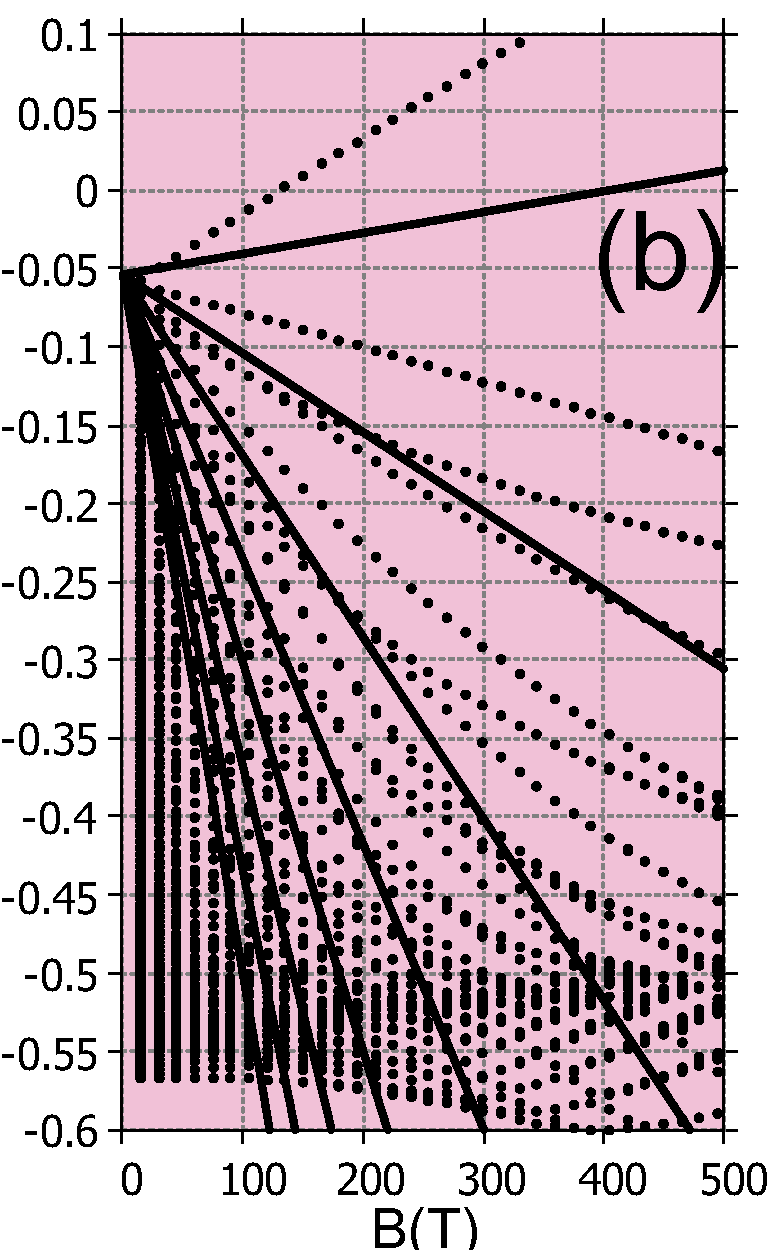
\includegraphics[width=0.85\textwidth,height=1.2\linewidth]{pic/landaulevel_3band_q_797_EF_approx_solution.pdf}}
%	\end{subfigure}
%	\begin{subfigure}[b]{0.49\textwidth}
%		\centering
%		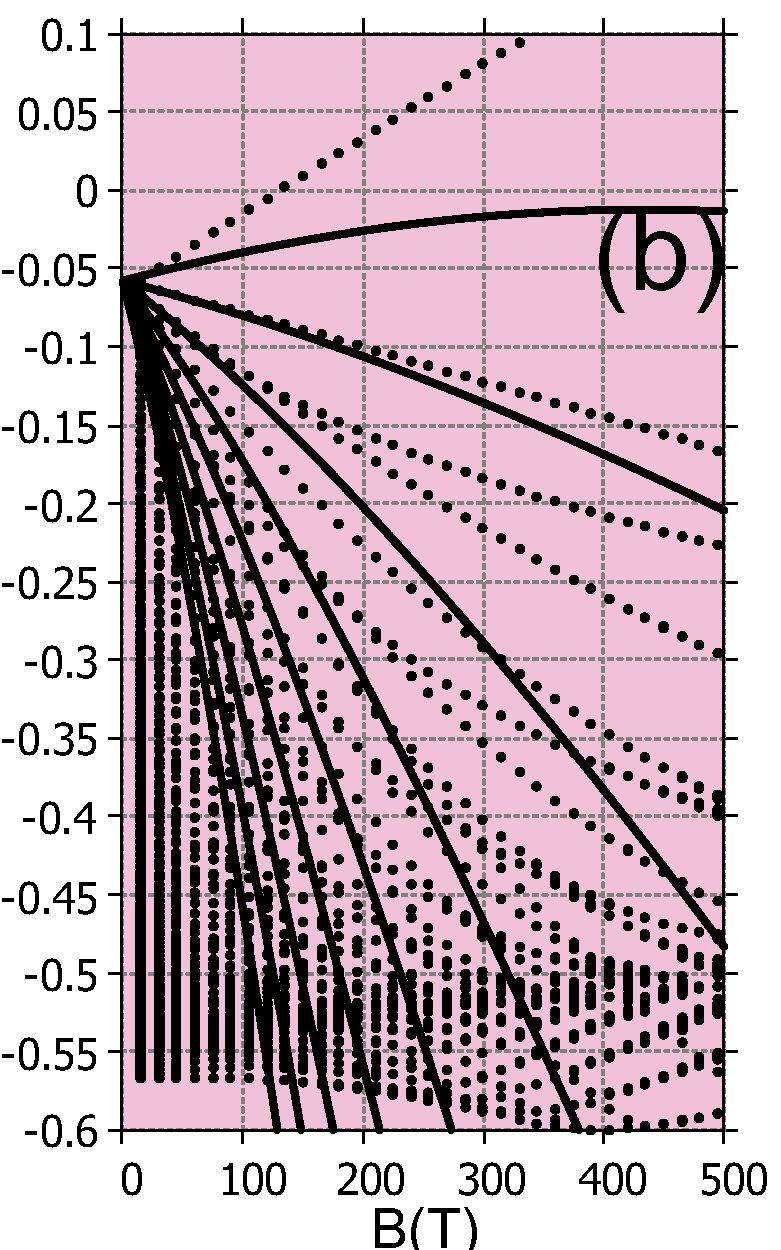
\includegraphics[width=0.85\textwidth,height=1.2\linewidth]{pic/landaulevel_3band_q_797_EF_analytics_solution.pdf}
%	\end{subfigure}
%	\caption{
%		A comparision bewteen two methods, figure on the right take data from maple, both depicts Landau levels.
%	}
%\end{figure*}
%\chapter{Fermi energy}
%Given
%\begin{gather}
%	E_{\lambda} = \frac{\hbar^{2} k^{2}}{2m} + \left(\lambda + \frac{1}{2}\right) \hbar \omega_{c},
%\end{gather}
%and
%\begin{gather}
%	n_{0} = \sum_{\lambda=0}^{\lambda_{\text{max}}} f(E_{F}) = \sum_{\lambda=0}^{\lambda_{\text{max}}} \tfrac{1}{\exp[\frac{E_{\lambda} - E_{F}}{k_{B}T}] + 1},
%\end{gather}
%In this work, we had choose $\lambda_{\text{max}} = 30$, if $\lambda \geq \lambda_{\text{max}}$ then $n_{0} = 0$ due to the property of Fermi level. With the aid of Eq (2.50), we rewrite (D.2) in the form as
%\begin{gather}
%	n_{0} = \sum_{ \lambda = 0}^{\lambda_{\text{max}}} \f{1}{\exp[\tfrac{t_{0} \left(6 - 8\pi\sqrt{3} \frac{p}{q}( \lambda + 1 /2)\right) + \epsilon_{1} - E_{F}}{k_{B} T}] + 1},
%\end{gather}
%with $k_{B}$ is Boltzmann constant, $T= 50$mK, $n_{0} = 2.8\times10^{15}$m$^{-2}$
%\begin{equation}
%	\begin{aligned}
%		E_{F} = - \ln\left[\frac{1-n_{0}}{n_{0}}\right] k_{B}T + E_{n}
%	\end{aligned}
%\end{equation}
%
%Density of states DOS $D(\varepsilon)$ is calculated from
%\begin{gather}
%	\rho(E_{F},T) = \int_{-\infty}^{E_{F}} f\left(\frac{\varepsilon - E_{F}}{k_{B}T}\right) D(\varepsilon) d\varepsilon,
%\end{gather}
%where $f(x) = \frac{1}{e^{x} + 1}$ is the Fermi-Dirac distribution, $T$ is the temperature of the system.













%\begin{equation}
%	\begin{aligned}
%		h_{v}
%		\approx & 3(t_{11} + t_{22}) - \f{3a^{2}(t_{11} + t_{22})}{4\hbar^{2}} \f{\hbar e B}{2} ( - a^{\dagger} a^{\dagger} + a^{\dagger}a + a a^{\dagger} - aa ) \\
%		        & - \f{3a^{2}(t_{11} + t_{22})}{4\hbar^{2}} \f{\hbar e B}{2} (aa + a a^{\dagger} + a^{\dagger} a + a^{\dagger} a^{\dagger})                       \\
%		        & - \f{a^{3} t_{12}}{4\hbar^{2}} \f{\hbar e B}{2} ( - a^{\dagger} a^{\dagger} + a^{\dagger}a + a a^{\dagger} - aa ) \Pi_{x}                       \\
%		        & + \f{a^{3} t_{12}}{4\hbar^{2}} \f{3\hbar e B}{2} ( a^{\dagger} a^{\dagger} + a^{\dagger}a + a a^{\dagger} + aa ) \Pi_{x} + \epsilon_{2}         \\
%		\approx & 3(t_{11} + t_{22}) - \f{3a^{2}(t_{11} + t_{22})}{4\hbar^{2}} \f{\hbar e B}{2}
%	\end{aligned}
%\end{equation}

%Tới đây thì không thể tính ra được vì còn số hạng bậc 3 theo kx ky và $i$ có nghĩa là vẫn còn $\Pi_{x}$. \\
%Tần số cyclotron khi sử dụng như section 2( đã loại bỏ số hạng có $a^3$ và $a^4$)
%\begin{gather}
%	w_{c} = \f{eB}{m^{*}} = \f{4 \pi \sqrt{3} (t_{11} + t_{22})}{\hbar} \f{p}{q},
%\end{gather}
%and
%\begin{gather}
%	E \approx (t_{11} + t_{22}) \left(3 - 4\pi \sqrt{3} \f{p}{q}(n + 1/ 2)\right) + \epsilon_{2},
%\end{gather}
%\begin{figure}[H]
%	\centering
%	\includegraphics[width=0.5\linewidth,height=0.5\linewidth]{pic/wrong.png}
%	\caption{\label{}  C.13}
%\end{figure}
%
%
%
%By using Taylor expansion, Hamiltonian Eq()
%\begin{equation}
%	\begin{aligned}
%		h_{0}  & = t_{0} (6 - \frac{3}{2} a^{2} (k_{x}^{2} + k_{y}^{2})) + \epsilon_{1}                                                                         \\
%		h_{1}  & = i t_{1} 3a k_{x} - \frac{3}{2} t_{2} a^{2} k_{x}k_{y}                                                                                        \\
%		h_{2}  & = 2 t_{2} (\frac{3}{8} a^{2} k_{x}^{2} + \frac{3}{8} a^{2} k_{y}^{2}) + i 3 t_{1} a k_{y}                                                      \\
%		h_{11} & = (t_{11} + 3 t_{22}) (1 - \frac{1}{8}a^{2} k_{x}^{2} - \frac{3}{8}a^{2} k_{y}^{2}) + 2 t_{11}(1 - \frac{1}{2} a^{2} k_{x}^{2}) + \epsilon_{2} \\
%		h_{22} & = (3 t_{11} + t_{22}) (1 - \frac{1}{8}a^{2} k_{x}^{2} - \frac{3}{8}a^{2} k_{y}^{2}) + 2 t_{22}(1 - \frac{1}{2} a^{2} k_{x}^{2}) + \epsilon_{2} \\
%		h_{12} & = \sqrt{3} (t_{22} - t_{11}) a^{2} k_{x} k_{y}
%		%+ 4i t_{12} \frac{a k_{x}}{2} ( \frac{3a^{2} k_{y}^{2}}{8} - \frac{a^{2} k_{x}^{2}}{8})
%	\end{aligned}
%\end{equation}
%By using substitution $\hbar \mathbf{k} = \boldsymbol{\Pi} + e \mathbf{A}$
%\begin{equation}
%	\begin{aligned}
%		h_{0}  & = t_{0} (6 - \frac{3}{2\hbar^{2}} a^{2} (\Pi_{x}^{2} + (\Pi_{y} + e Bx)^{2})) + \epsilon_{1}                                                                 \\
%		h_{1}  & = i t_{1} \frac{3}{\hbar}a \Pi_{x} - \frac{3}{2\hbar^{2}} t_{2} a^{2} \Pi_{x}(\Pi_{y} + eBx)                                                                 \\
%		h_{2}  & = 2 t_{2} (\frac{3}{8\hbar^{2}} a^{2} \Pi_{x}^{2} + \frac{3}{8\hbar^{2}} a^{2} (\Pi_{y} + eBx)^{2}) + i \frac{3}{\hbar} t_{1} a (\Pi_{y} + eBx)              \\
%		h_{11} & = (t_{11} + 3 t_{22}) (1 - \frac{1}{8}a^{2} \Pi_{x}^{2} - \frac{3}{8}a^{2} (\Pi_{y} + eBx)^{2}) + 2 t_{11}(1 - \frac{1}{2} a^{2} \Pi_{x}^{2}) + \epsilon_{2} \\
%		h_{22} & = (3 t_{11} + t_{22}) (1 - \frac{1}{8}a^{2} \Pi_{x}^{2} - \frac{3}{8}a^{2} (\Pi_{y} + eBx)^{2}) + 2 t_{22}(1 - \frac{1}{2} a^{2} \Pi_{x}^{2}) + \epsilon_{2} \\
%		h_{12} & = \sqrt{3} (t_{22} - t_{11}) a^{2} \Pi_{x} (\Pi_{y} + eBx)
%		%+ 4i t_{12} \frac{a k_{x}}{2} ( \frac{3a^{2} k_{y}^{2}}{8} - \frac{a^{2} k_{x}^{2}}{8})
%	\end{aligned}
%\end{equation}
%Hamiltonian in term of ladder operators
%\begin{equation}
%	\begin{aligned}
%		h_{0} &= -6t_{0}a^{2}( a^{\dagger} a^{-} + \tfrac{1}{2}) + 6t_{0} + \epsilon_{1} \\
%		h_{1} &= 3 t_{1} a ( a^{-} - a^{\dagger}) - \tfrac{3 i t_{2} a^{2}}{2}(a^{\dagger} a^{\dagger} - a^{-}a^{-} - 1) \\
%		h_{2} &= 3 i t_{1} a (a^{\dagger} + a^{-}) + \tfrac{3t_{2} a^{2}}{2}(a^{\dagger} a^{\dagger} + a^{-} a^{-})\\
%		h_{11} &=	3 (t_{11} + t_{22}) + \tfrac{3t_{11}a^{2}}{4}( a^{\dagger}a^{\dagger} + a^{-} a^{-} ) - 3 (t_{11} + t_{22})a^{2} (a^{\dagger} a^{-} + \tfrac{1}{2}) + \epsilon_{2} \\
%		h_{22} &=	3 (t_{11} + t_{22}) + \tfrac{3t_{22}a^{2}}{4}( a^{\dagger}a^{\dagger} + a^{-} a^{-} ) - 3 (t_{11} + t_{22})a^{2} (a^{\dagger} a^{-} + \tfrac{1}{2}) + \epsilon_{2} \\
%		h_{12} &= \sqrt{3}i (t_{22} - t_{11}) (a^{\dagger} a^{\dagger} - a^{-} a^{-} - 1) 
%	\end{aligned}
%\end{equation}





%\chapter{Phase factor}
%\begin{equation}
%	\begin{aligned}
%		H_{\mu\mu'}^{jj'}(\mathbf{k})
%		& = \sum_{\mathbf{R}} e^{\frac{ie}{\hbar}\int_{0}^{\mathbf{R}}A(\mathbf{r'})d\mathbf{r'}}e^{i\mathbf{k\cdot R}} E_{\mu\mu'}^{jj'}(\mathbf{R})                                                                                                                                                   \\
%		& = E_{\mu\mu'}^{jj'}(\mathbf{0}) + e^{\frac{ie}{\hbar}\int_{0}^{\mathbf{R_1}}\mathbf{A(\mathbf{r'})}\cdot d\mathbf{r'}}e^{i\mathbf{k\cdot R_1}} E_{\mu\mu'}^{jj'}(\mathbf{R_1})                                                                                                                \\
%		& + e^{\frac{ie}{\hbar}\int_{0}^{\mathbf{R_2}}\mathbf{A(\mathbf{r'})}\cdot d\mathbf{r'}}e^{i\mathbf{k\cdot R_2}} E_{\mu\mu'}^{jj'}(\mathbf{R_2}) + e^{\frac{ie}{\hbar}\int_{0}^{\mathbf{R_3}}\mathbf{A(\mathbf{r'})}\cdot d\mathbf{r'}}e^{i\mathbf{k\cdot R_3}} E_{\mu\mu'}^{jj'}(\mathbf{R_3}) \\
%		& + e^{\frac{ie}{\hbar}\int_{0}^{\mathbf{R_4}}\mathbf{A(\mathbf{r'})}\cdot d\mathbf{r'}}e^{i\mathbf{k\cdot R_4}} E_{\mu\mu'}^{jj'}(\mathbf{R_4}) + e^{\frac{ie}{\hbar}\int_{0}^{\mathbf{R_5}}\mathbf{A(\mathbf{r'})}\cdot d\mathbf{r'}}e^{i\mathbf{k\cdot R_5}} E_{\mu\mu'}^{jj'}(\mathbf{R_5}) \\
%		& + e^{\frac{ie}{\hbar}\int_{0}^{\mathbf{R_6}}\mathbf{A(\mathbf{r'})}\cdot d\mathbf{r'}}e^{i\mathbf{k\cdot R_6}} E_{\mu\mu'}^{jj'}(\mathbf{R_6})\\
%		&=  E_{\mu\mu'}^{jj'}(\mathbf{0}) + e^{\frac{ie}{\hbar} Bx \int_{\mathbf{0}}^{\mathbf{R}_{1}}dy} e^{i k_{x} a} E_{\mu\mu'}^{jj'}(\mathbf{R}_{1}) + e^{\frac{ie}{\hbar} Bx \int_{\mathbf{0}}^{\mathbf{R}_{2}}dy} e^{i k_{x}\frac{a}{2}} e^{-i k_{y} \frac{a\sqrt{3}}{2}} E_{\mu\mu'}^{jj'}(\mathbf{R}_{2}) \\
%		&+ e^{\frac{ie}{\hbar} Bx \int_{\mathbf{0}}^{\mathbf{R}_{3}}dy} e^{-i k_{x} \frac{a}{2}} e^{-i k_{y} \frac{a\sqrt{3}}{2}} E_{\mu\mu'}^{jj'}(\mathbf{R}_{3}) + e^{\frac{ie}{\hbar} Bx \int_{\mathbf{0}}^{\mathbf{R}_{4}}dy} e^{-i k_{x} a} E_{\mu\mu'}^{jj'}(\mathbf{R}_{4})\\
%		&+ e^{\frac{ie}{\hbar} Bx \int_{\mathbf{0}}^{\mathbf{R}_{5}}dy} e^{-i k_{x} a} e^{i k_{y} \frac{a\sqrt{3}}{2}} E_{\mu\mu'}^{jj'}(\mathbf{R}_{5}) + e^{\frac{ie}{\hbar} Bx \int_{\mathbf{0}}^{\mathbf{R}_{6}}dy} e^{i k_{x} a} e^{i k_{y} \frac{a\sqrt{3}}{2}} E_{\mu\mu'}^{jj'}(\mathbf{R}_{6})\\
%		&=  E_{\mu\mu'}^{jj'}(\mathbf{0}) + e^{0} e^{i k_{x} a} E_{\mu\mu'}^{jj'}(\mathbf{R}_{1}) + e^{-\frac{ie}{\hbar} B x \frac{a\sqrt{3}}{2}} e^{i k_{x}\frac{a}{2}} e^{-i k_{y} \frac{a\sqrt{3}}{2}} E_{\mu\mu'}^{jj'}(\mathbf{R}_{2}) \\
%		&+ e^{-\frac{ie}{\hbar} B x \frac{a\sqrt{3}}{2}} e^{-i k_{x} \frac{a}{2}} e^{-i k_{y} \frac{a\sqrt{3}}{2}} E_{\mu\mu'}^{jj'}(\mathbf{R}_{3}) + e^{0} e^{-i k_{x} a} E_{\mu\mu'}^{jj'}(\mathbf{R}_{4})\\
%		&+ e^{\frac{ie}{\hbar} B x \frac{a\sqrt{3}}{2}} e^{-i k_{x} a} e^{i k_{y} \frac{a\sqrt{3}}{2}} E_{\mu\mu'}^{jj'}(\mathbf{R}_{5}) + e^{\frac{ie}{\hbar} B x \frac{a\sqrt{3}}{2}} e^{i k_{x} a} e^{i k_{y} \frac{a\sqrt{3}}{2}} E_{\mu\mu'}^{jj'}(\mathbf{R}_{6})
%	\end{aligned}
%\end{equation}
%Applying the BCH formula, and using the commutation relation $\left[x, p_{x}\right] = i \hbar$, we have
%\begin{equation}
%	\begin{aligned}
%		e^{i\left( \frac{\hbar k_{x}}{\hbar} - \frac{e}{\hbar}Bx \sqrt{3}\right) \frac{a}{2}}
%		= e^{i\left( p_{x} - \sqrt{3}eBx\right) \frac{a}{2 \hbar}} = 
%	\end{aligned}
%\end{equation}
%\chapter{Matrix}
%
%\begin{equation}
%	\rotatebox{90}{$
%		\begin{aligned}
%			h_{1}
%			& =
%			\begin{pNiceArray}{c|c|c|c|c|c|c|c}
%				\scriptstyle 0                    & \Block{1-1}{\scriptstyle 2t_{1}\cos\zeta_{1}  \\ \scriptstyle + i \sqrt{3} t_{2} \sin\zeta_{1}}   &\scriptstyle t_{1}               & \scriptstyle 0                   & \cdots & \scriptstyle 0                    & \scriptstyle -t_{1}                & \Block{1-1}{\scriptstyle -2t_{1}\cos\gamma_{1}  \\ \scriptstyle - i \sqrt{3} t_{2} \sin\gamma_{1}} \\
%				\hline
%				\Block{1-1}{\scriptstyle -2t_{1}\cos\gamma_{2}  \\ \scriptstyle - i \sqrt{3} t_{2} \sin\gamma_{2}} & \scriptstyle 0                     & \Block{1-1}{\scriptstyle 2t_{1}\cos\zeta_{2}  \\ \scriptstyle + i \sqrt{3} t_{2} \sin\zeta_{2}} &\scriptstyle t_{1}               & \scriptstyle 0      & \cdots               & \scriptstyle 0                    & \scriptstyle -t_{1}                \\
%				\hline
%				\scriptstyle -t_{1}                & \Block{1-1}{\scriptstyle -2t_{1}\cos\gamma_{3}  \\ \scriptstyle - i \sqrt{3} t_{2} \sin\gamma_{3}} & \scriptstyle 0                   & \Block{1-1}{\scriptstyle 2t_{1}\cos\zeta_{3}  \\ \scriptstyle + i \sqrt{3} t_{2} \sin\zeta_{3}} &\scriptstyle t_{1}  & \scriptstyle 0                    & \cdots                    & \scriptstyle 0                    \\
%				\hline
%				\vdots               & \vdots                & \vdots              & \vdots              & \vdots & \vdots               & \vdots               & \vdots               \\
%				\hline
%				t_{1}                & \scriptstyle 0                     & \cdots              & \scriptstyle 0                   & \scriptstyle -t_{1}  & \Block{1-1}{\scriptstyle -2t_{1}\cos\gamma_{q - 1}  \\ \scriptstyle - i \sqrt{3} t_{2} \sin\gamma_{q - 1}} & \scriptstyle 0                    & \Block{1-1}{\scriptstyle 2t_{1}\cos\zeta_{q - 1}  \\ \scriptstyle + i \sqrt{3} t_{2} \sin\zeta_{q - 1}}  \\
%				\hline
%				\Block{1-1}{\scriptstyle 2t_{1}\cos\zeta_{q}  \\ \scriptstyle + i \sqrt{3} t_{2} \sin\zeta_{q}}  &\scriptstyle t_{1}                 & \cdots              & \scriptstyle 0                   & \scriptstyle 0      & \scriptstyle -t_{1}                & \Block{1-1}{\scriptstyle -2t_{1}\cos\gamma_{q}  \\ \scriptstyle - i \sqrt{3} t_{2} \sin\gamma_{q}} & \scriptstyle 0                    \\
%			\end{pNiceArray}
%		\end{aligned}$}
%\end{equation}


%\nocite{*}
\begingroup
  \renewcommand{\bibname}{REFERENCES}
  \def\addcontentsline#1#2#3{}  % chặn thêm vào TOC
  \bibliographystyle{unsrt}
  \bibliography{refs}
\endgroup

\end{document}
